\documentclass{sig-alternate}

\usepackage{amssymb,amsmath}
\usepackage{wrapfig}
\usepackage{multirow}
\usepackage{graphicx}
\usepackage{algorithm}
\usepackage{algorithmic}
\usepackage{times}
\usepackage{cite}
\usepackage{url}
\usepackage{booktabs}
\usepackage{subfigure}
\usepackage{fancybox}
\usepackage{color}
\usepackage{array}
\usepackage{subfigure}
\usepackage{balance}
\usepackage{epstopdf}
\usepackage{array}
\usepackage{xspace}
\usepackage{makecell}
\usepackage{siunitx}


% author comments with colors 
\newcommand{\emad}[1]{\textcolor{red}{{\it [Emad: #1]}}}
\newcommand{\nikos}[1]{\textcolor{red}{{\it [Nikos: #1]}}}
\newcommand{\everton}[1]{\textcolor{blue}{{\it [Everton: #1]}}}
\newcommand{\todo}[1]{\colorbox{yellow}{\textbf{[#1]}}}

% conclusion box for summarize the research questions
\newcommand{\conclusionbox}[1]{%
       \vspace{2mm}
       \framebox[0.45\textwidth][c]{%
              \parbox[b]{0.42\textwidth}{%
                     {\it #1}
              }
       }
       \vspace{2mm}
}

% research questions 
\newcommand{\rqi}{\textbf{RQ1. Is it possible to effectively identify/predict \SATD using NLP techniques ?\\}}
\newcommand{\rqii}{\textbf{RQ2. What are the most common comment patterns that indicates \SATD ?\\}}
\newcommand{\rqiii}{\textbf{RQ3. How much training data is necessary for successfully predict \SATD ?\\}}

% commands for common terms in the text

\newcommand{\SATD}{self-admitted technical debt\xspace}


\begin{document}

% --- Author Metadata here ---
% \conferenceinfo{WOODSTOCK}{'97 El Paso, Texas USA}
%\CopyrightYear{2007} % Allows default copyright year (20XX) to be over-ridden - IF NEED BE.
%\crdata{0-12345-67-8/90/01}  % Allows default copyright data (0-89791-88-6/97/05) to be over-ridden - IF NEED BE.
% --- End of Author Metadata ---

\title{Using Source Code Comments to Detect Self-Admitted Technical Debt}

\numberofauthors{1} 
\author{
\alignauthor 
       Everton da S. Maldonado, Nikolaos Tsantalis and Emad Shihab\\
       \affaddr{Department of Computer Science and Software Engineering}\\
       \affaddr{Concordia University, Montreal, Canada }\\
       \email{e\_silvam@encs.concordia.ca, nikolaos.tsantalis@concordia.ca, emad.shihab@concordia.ca}
% 2nd. author
% \alignauthor 
%        Second Author\\
%        \affaddr{Department of Computer Science and Software Engineering}\\
%        \affaddr{Concordia University}\\
%        \affaddr{Montreal, Canada}\\
%        \email{2autor@encs.concordia.ca}
% % 3rd. author
% \alignauthor 
%        Third author\\
%        \affaddr{Department of Computer Science and Software Engineering}\\
%        \affaddr{Concordia University}\\
%        \affaddr{Montreal, Canada}\\
%        \email{3author@encs.concordia.ca}
}


\maketitle
\begin{abstract}
During the development and maintenance of a software system, developers face unpredictable difficulties or pressures, and in many cases are forced to apply unconventional solutions to overcome these difficulties. For example, they might adopt insufficiently tested or temporary solutions (i.e., workarounds and hacks), neglect good design practices, and introduce inaccurate or incomplete documentation due to time constraints and pressure to meet deadlines. This phenomenon has been explained through the metaphor of Technical Debt. 

More recently, our work shown that one possible source to detect technical debt is using source code comments, also referred to as self-admitted technical debt. In addition to that, we pointed out that the most common types of self-admitted technical debt found in comments are design technical debt, requirement debt and defect debt. 

Therefore, in this paper we present an approach to efficiently identify these types of self-admitted technical debt. 
% More specifically,  using natural language processing techniques. 

\end{abstract}

% A category with the (minimum) three required fields
% \category{H.4}{Information Systems Applications}{Miscellaneous}
%A category including the fourth, optional field follows...
% \category{D.2.8}{Software Engineering}{Metrics}[complexity measures, performance measures]

\terms{}

\keywords{}

\section{Introduction}
\label{sec:introduction}

Developers often have to deal with conflicting goals that require software to be delivered quickly, with high quality, and on budget. In practice, achieving all of these goals at the same time can be challenging, causing a tradeoff to be made. Often, these tradeoffs lead developers to take \emph{shortcuts} or use \emph{workarounds}. Although such shortcuts help developers in meeting their short-term goals, they may have a negative impact in the long-term.

Technical debt is a metaphor that has been used to express sub-optimal solutions that are taken consciously in a software project in order to achieve some short-term goals. Generally, these decisions allow the project to move faster in the short-term, but introduce an increased cost (i.e., debt) to maintain this software in the long run~\cite{Seaman2011,Kruchten2013IWMTD}. Prior work showed that technical debt is widespread in the software domain, is unavoidable, and can have a negative impact on the quality of the software~\cite{Lim2012Software}.

Due to the importance of technical debt, a number of studies empirically examined it and proposed techniques to enable its detection and management. The main findings of the prior work is that 1) there are different types of technical debt, e.g., defect debt, design debt, testing debt, and that design debt has the highest impact~\cite{Alves2014MTD,Marinescu2012IBM}; and 2) statically analyzing the source code can help detecting technical debt~\cite{Marinescu2004ICSM,Marinescu2010CSMR,Zazworka2013CSE}. In particular, these works use metric thresholds to detect code smells, which are considered as proxies for technical debt. 

One major drawback of using metrics to detect technical debt is that no one knows if the detected smells really constitute technical debt, or if they correspond to problems that the developers care about. Therefore, more recently, our work showed that using code comments can be effective in identifying self-admitted technical debt~\cite{Potdar2014ICSME}. This work uses comments to detect \emph{generic} technical debt, and did not focus on any specific type of technical debt.


\begin{figure*}[thb!]
    \centering
    \label{fig:approach}
    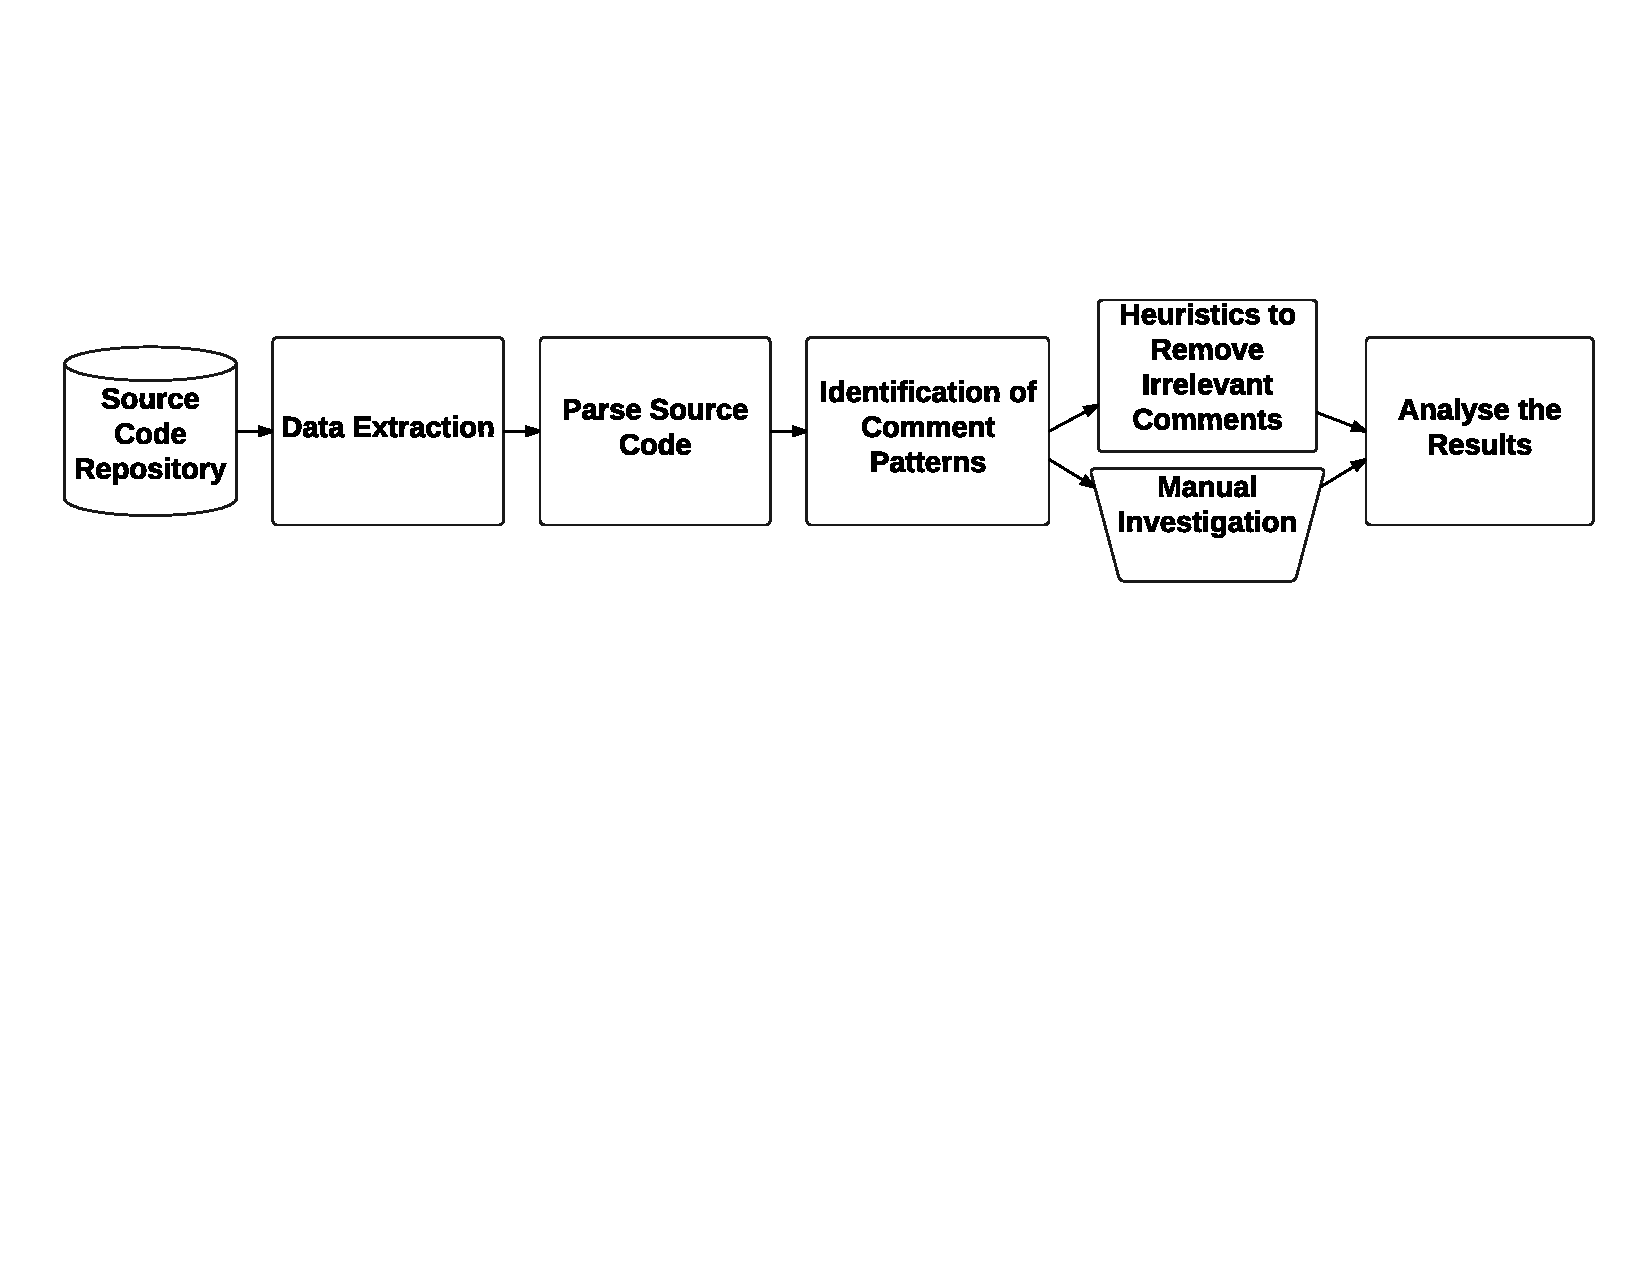
\includegraphics[width=1\textwidth]{figures/Approach2}
    %Caption goes below the figure
    \vspace{-10mm}
    \caption{Approach overview}
\end{figure*}


In this paper, we build on the promising approach of using code comments to detect one of the most impacting types of debt, namely \emph{design technical debt}, which we call \SADTD. We manually examine more than 17,000 code comments to extract comment patterns that can be used to detect \SADTD. To examine the effectiveness of our approach, we perform an empirical study on ten open source projects. Finally, we compare our approach to state-of-the-art approaches and examine the effectiveness of using automated refactoring techniques in mitigating \SADTD.

Based on our manual examination of the code comments, we derive 176 different comment patterns that can be used to detect \SADTD. These patterns are able to detect \SADTD with a precision ranging in 74.0-96.30\% and a recall ranging in 10.87-83.87\%. Moreover, we find that the design technical debt found with our approach is different than the design technical debt found using metric-based approaches~\cite{Zazworka2013CSE}. Finally, we find that automated refactoring can address up to 24.58\% of the methods containing \SADTD.

%Despite its utility this approach has one major limitation.
%There is no way to be sure that the detected code smells are indeed problems that the developers care about, and their resolution is absolutely necessary for the survival of the project.
%Many different refactorings opportunities can appear while analyzing a piece of source code, but it is still an open problem
%to determine the refactorings that should be recommended with higher priority, because they are more important for the developers.
%%Nikos: This is our big statement. I would even put it in emphasis
%\emph{Self-admitted design debt could be the missing element to guide the process of refactoring recommendation.}


%In particular, we would like to answer the following two research questions:
%
%\noindent\rqi 
%\everton{Explain in detail the different nature of each approach}
%We extracted 176 comment patterns that can identify \SADTD~in the source code.
%\nikos{The text that follows is ugly and unclear}
%While comparing the \SADTD~patterns with the more general Debt patterns, defined in \cite{Potdar2014ICSME}, we found that they have essentially different mechanics although some of the patterns that is found in one can also be found in the other one.
%All of the positive matches that the general Self-Admitted Technical Debt patterns generated was also contained in the \SADTD~ patterns matches. Which means that the more specific \SADTD~patterns made obsolete the general Self-Admitted Technical Debt patterns, regarding design debt. 
%
%\noindent\rqii
%\nikos{The same here! It's not even clear how we computed precision and recall}
%We find that our highest precision value has of 88.57\% in Squirrel SQL Client project and our lowest mark was of 74.07\% in Columba project. We achieved an high overall precision of 84.93\%. The overall recall measured was of 19.01\% Therefore our highest result while measuring recall was of 27.16\% in Jmeter and our lowest result was 10.87\% in JFreeChart.


The rest of the paper is organized as follows:  Section~\ref{sec:motivating_example} presents a motivating example. Section~\ref{sec:approach} details our approach. We present our case study results in Section~\ref{sec:case_study_results}, followed by a discussion in Section \ref{sec:discussion}. Section~\ref{sec:related_work} presents the related work. The threats to validity of our work are discussed in Section~\ref{sec:threats_to_validity}. Section~\ref{sec:conclusion} lists the conclusions of our work.

\section{Motivating Example}
\label{sec:motivating_example}
As mentioned earlier, one of the first works on self-admitted technical debt was the work by Potdar and Shihab~\cite{Potdar2014ICSME}. Their work showed that it is possible to identify self-admitted technical debt using source code comments. However, in their work, Potdar and Shihab studied \textit{generic} technical debt, i.e., they did not discriminate between the different types of technical debt. For example, technical debt can be in the form of design debt, testing debt, defect debt, and documentation debt. 

Since our work focuses on \SADTD, we first examined the effectiveness of using the general comments used by Potdar and Shihab to detect design technical debt. We applied the comment patterns that we derived (which we present later in the paper) and the comment patterns from Potdar and Shihab on the studied open source projects. As expected, the results produced by the general comment patterns identified all types of technical debt, indicating the need for more specific comment patterns that can be used to effectively identify design technical debt.

To illustrate our point, we show some example comments flagged by Potdar and Shihab's approach in the first column of Table~\ref{tab:satdmotivation}. The second column of the table shows the comments that are detected by the comment patterns we propose in this paper, which focus on \SADTD. A comparison of the comments in Table~\ref{tab:satdmotivation} clearly shows that the more specific comment patterns detect design issues. 

This simple example shows that comment patterns that specifically target design technical debt are needed. Simply using the general comment patterns may yield unfavourable results. We elaborate more on the performance of using the general comment patterns to detect \SADTD in Section~\ref{sec:case_study_results}.

\begin{table*}[!hbt]
    \begin{center}
        \caption{Example of General/Design Self-admitted Technical Debt Comments}
        \vspace{-2mm}
        \label{tab:satdmotivation}
        \begin{tabular}{ p{3in} | p{3in} } 
            \toprule
            \textbf{General Self-Admitted Technical Debt} &  \textbf{Self-Admitted Design Technical Debt}  \\ 
            \midrule
            \textit{remove this code once bug 62405 is fixed for the mainstream GTK} & \textit{This can lead to code smell, meh! Do we care}\\
            \textit{FIXME - This caching thing should not be here; it's brittle.} & \textit{This is an absurdly long method! Break it up.}\\
            \textit{FIXME compat: updateActionBars : should do something useful} & \textit{there should be an interface, instead of the         AbstractMessageFolder}\\
            \textit{FIXME this does not actually set the default since it is the wrong} & \textit{rethink where exactly some of the following methods belong (GenModel or GenPackage)}\\
            \textit{TODO: - please add some javadoc - ugly classname also} & \textit{Cyclic dependency with PersistenceManager}\\

            %\textit{FIXME: this is killing at least SSE editors, see bug 318034} & \textit{hack to support dockable view title update replace with listener pattern}\\
            %\textit{FIXME: this is not 64-bit clean} & \textit{This is in the wrong place.  It's not profile specific. It needs to be moved to main XMI reading code. }\\
            %\textit{HACK. Calling super.read() installs a required preferences change listener.} & \textit{This appears unused.  If it's needed, the Model API should be enhanced to provide a method that does this directly.}\\
            %\textit{This test is problematic. It makes assumptions about the behavior} & \textit{What does the magic number 6000 represent here? Put it in an explanatory literal! }\\
            %\textit{TODO: Won't our use of PathComparator take care of uniqueness?} & \textit{Downcast to avoid using an interface?  Yuck.}\\
            %\textit{FIXME: why override if nobody uses?} & \textit{We should actually rework this class to not implement Parser}\\
            %\textit{not exist yet. Throws a CoreException if there is a problem} & \textit{unhappy about this being public ... is there a better way?}\\
            %\textit{TODO this is such a hack it is silly.  There are still cases for race conditions etc} & \textit{remove use of instanceof!}\\
            %\textit{KLUDGE!! Test commented out until bug 170353 is fixed...} & \textit{a design flaw, it doesn't update properly}\\
            \bottomrule
        \end{tabular}
    \end{center}
\end{table*}

\section{Approach}
\label{sec:approach}
\begin{figure*}[thb!]
  \centering
  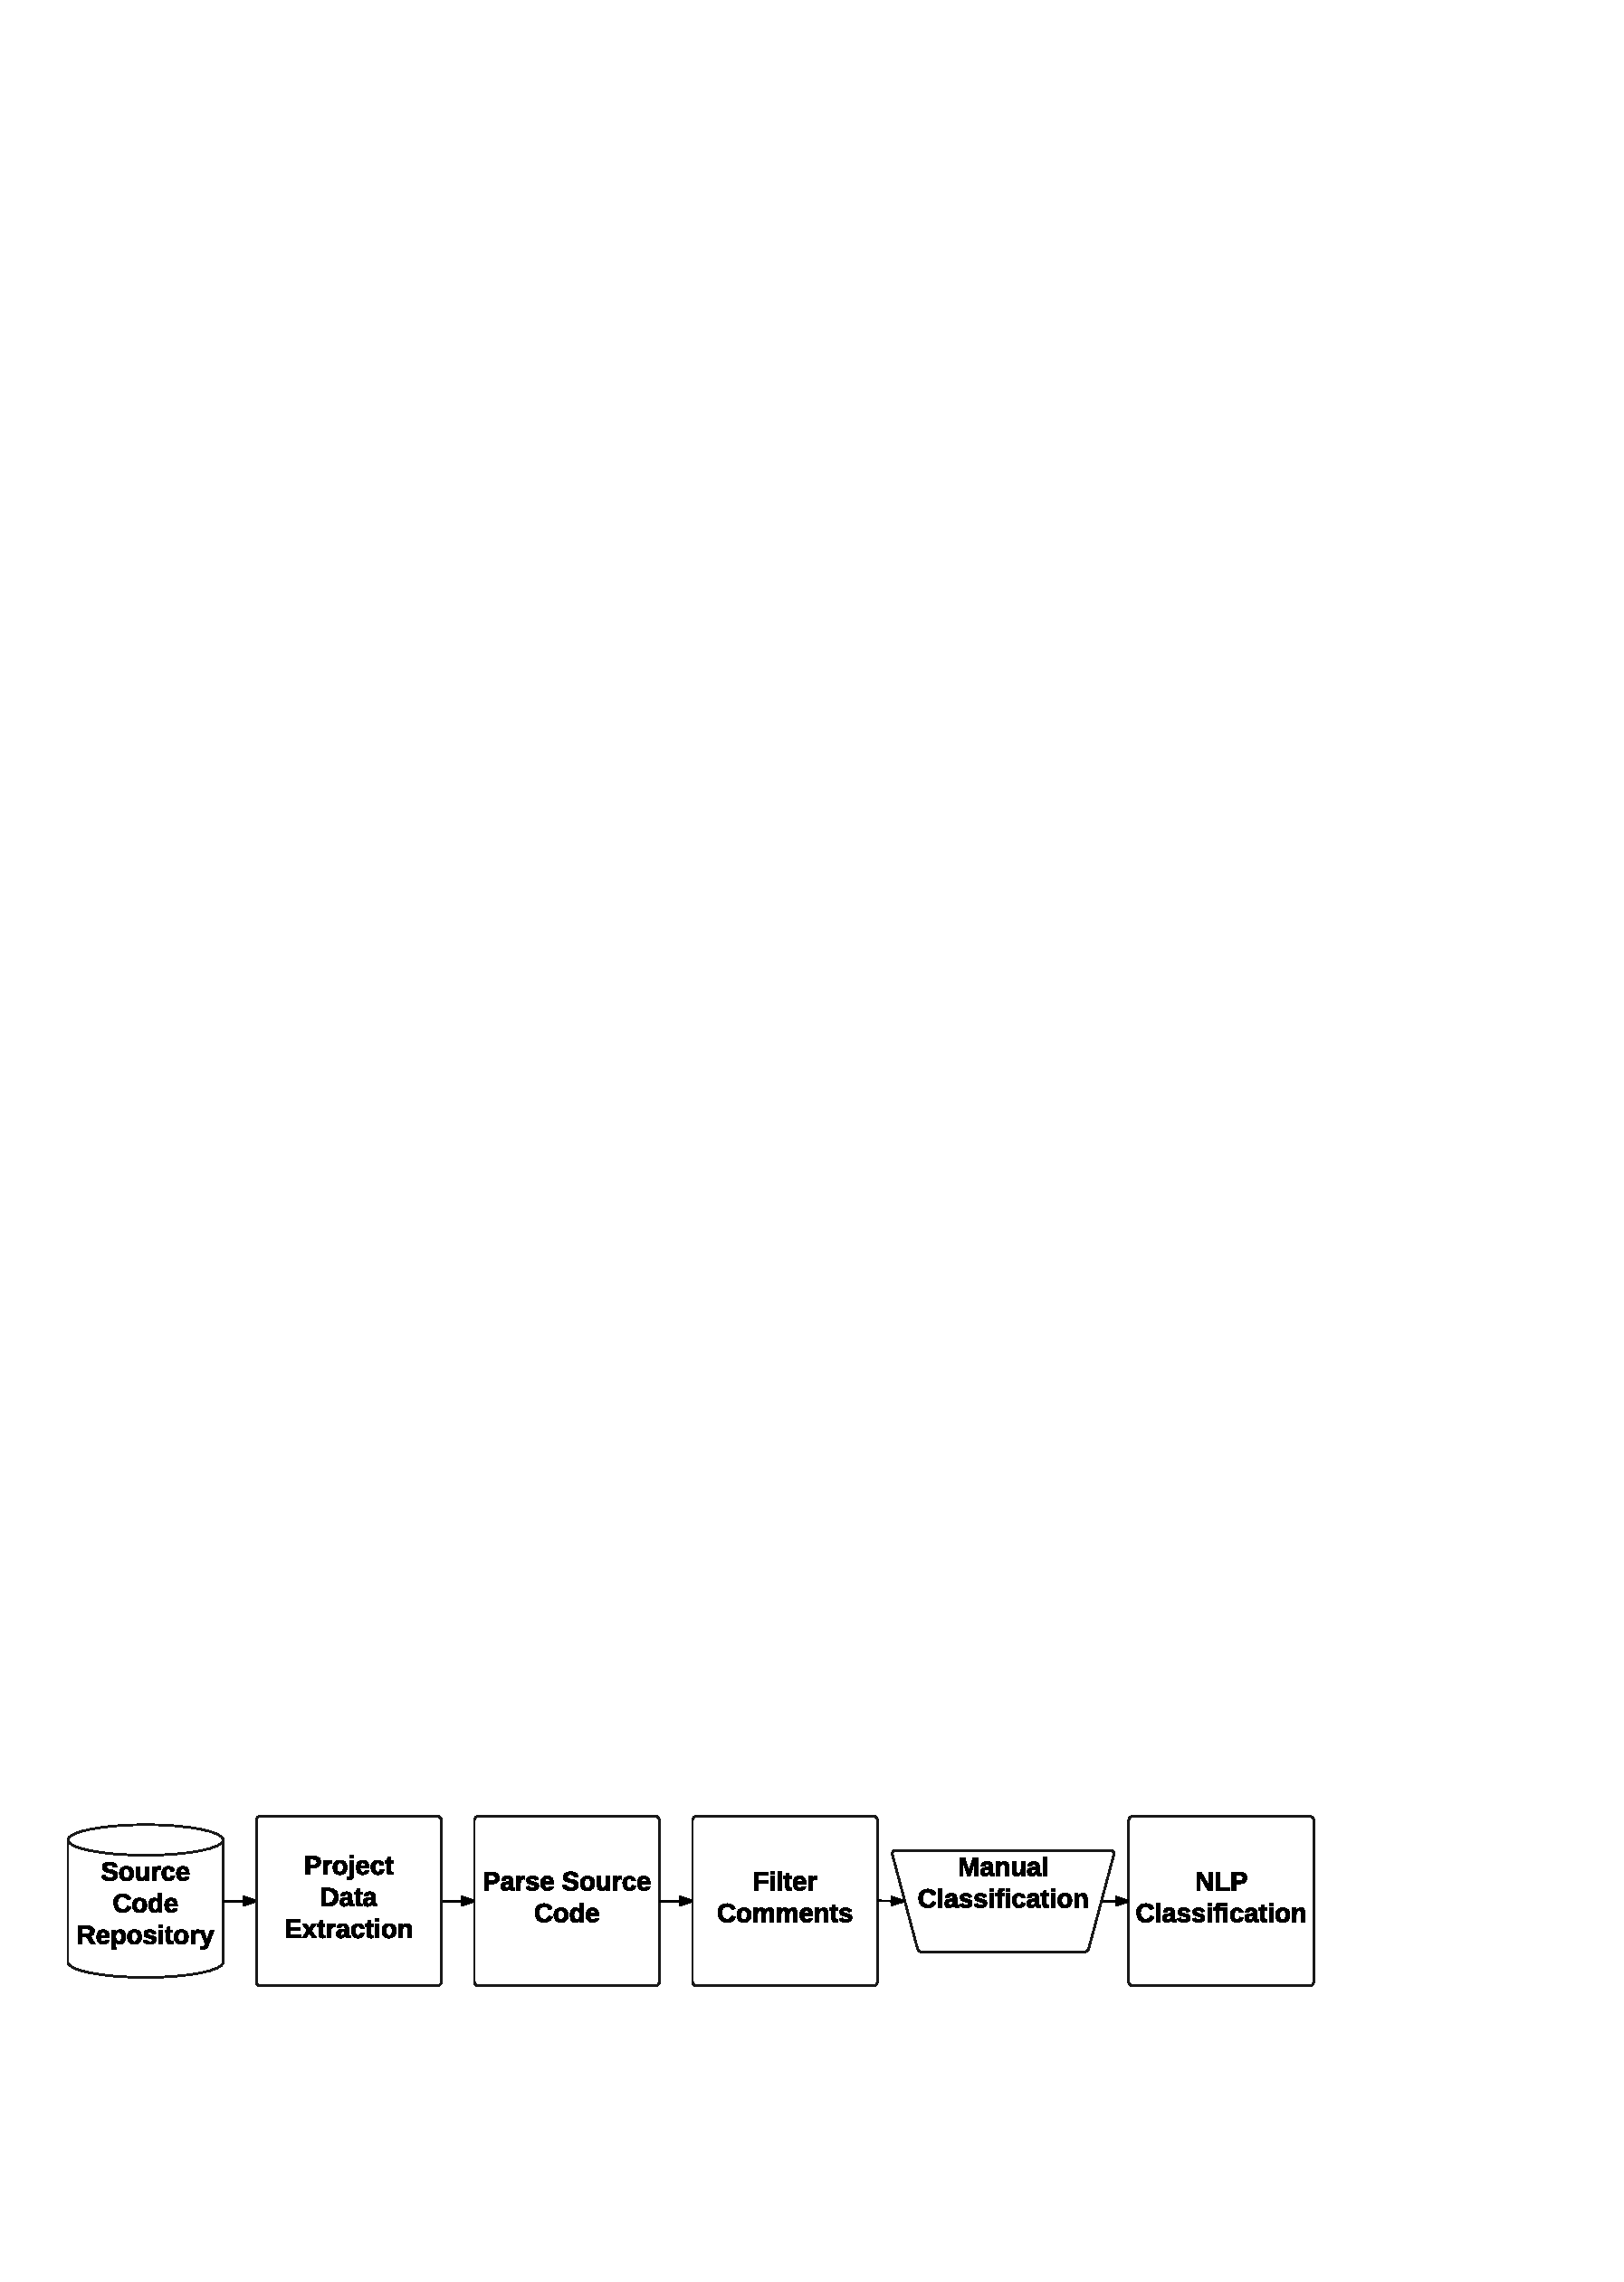
\includegraphics[width=1\textwidth]{figures/approach_reviwed.pdf}
  \caption{Approach Overview}
  \label{fig:approach}
  \vspace{-4mm}
\end{figure*}

The main goal of our study is to automatically identify \SATD through source code comments. To do that, we first extract the comments from ten open source projects. Second, we apply five filtering heuristics to remove comments that are irrelevant for the identification of \SATD  (e.g., license comments, commented source code and Javadoc comments). After that, we manually classify the remaining comments into the different types of \SATD (i.e., design debt, requirement debt, defect debt, documentation debt and test debt). Lastly, we use these comments as training data for the Stanford NLP Classifier and use the trained model to detect \SATD from source code comments. Figure~\ref{fig:approach} shows an overview of our approach, and the following subsections detail each step.

\subsection{Project Data Extraction} % (fold)
\label{sub:data_extraction}

To perform our study, we need to analyze the source code comments of software projects. Therefore, we extract the source code of ten open source projects, namely Ant, ArgoUML, Columba, EMF, Hibernate, JEdit, JFreeChart, Jmeter, JRuby and SQuirrel SQL. We selected these projects since they belong to different application domains, are well commented, vary in size, and in the number of contributors. 

Table~\ref{tab:project_details} provides details about each of the projects used in our study. The columns of Table~\ref{tab:project_details} present the release used, followed by the number of classes, the total source lines of code (SLOC), the number of contributors, the number of extracted comments, the number of comments analyzed after applying our filtering heuristics, the number of comments that were classified as \SATD, the percentage of these comments that represent design debt, the percentage of \SATD comments classified as requirement debt and finally the percentage of all other types of debt (i.e., defect, documentation and test debt). 

Since there are many different definitions for the SLOC metric we clarify that, in our study, a source line of code contains at least one valid character, which is not a blank space or a source code comment. In addition, we only use the Java files to calculate the SLOC, and to do so, we use the SLOCCount tool~\cite{wheeler2004:home}. 

The number of contributors was extracted from OpenHub, an on-line community and public directory that offers analytics, search services and tools for open source software \cite{Openhub:home}. It is important to note that the number of comments shown for each project does not represent the number of commented lines, but rather the number of Single-line, Block and Javadoc comments. In total, we obtained 259,229 comments, found in 16,249 Java classes. The size of the selected projects varies between 81,307 and 228,191 SLOC, and the number of contributors of these projects ranges from 9 to 326. 


\begin{table*}[thb!]
    \begin{center}
    \caption{Details of Studied Projects}
    \label{tab:project_details}
    \vspace{-5mm}
            \begin{tabular}{l| c c r c || c c c || c c c}
            \toprule
            
            \multirow{5}{*}{\textbf{\thead{Project}}} & \multicolumn{4}{c||}{\textbf{\thead{Project details}}} & \multicolumn{3}{c||}{\textbf{\thead{Comments details}}} & \multicolumn{3}{c}{\textbf{\thead{Technical Debt details}}}

            \\
            \cmidrule{2-11}

            & \textbf{\thead{Release}}  & \textbf{\thead{\# of classes}}   & \textbf{\thead{SLOC}} & \textbf{\thead{\# of \\contributors}}  & \textbf{\thead{\# of \\comments}}   & \textbf{\thead{\# of \\comments \\after filtering}} & \textbf{\thead{\# of \\TD \\comments}} & \textbf{\thead{\% of \\Design \\Debt}} & \textbf{\thead{\% of \\Requirement \\Debt}} & \textbf{\thead{\% of \\Other \\Debts}}\\ 
            \midrule 
            \textbf{Ant}            & 1.7.0    & 1,475 & 115,881 & 74  & 21,587 &   4,137 &    131 &  72.51  & 09.92  & 17.55 \\
            \textbf{ArgoUML}        & 0.34     & 2,609 & 176,839 & 87  & 67,716 &   9,548 &  1,413 &  56.68  & 29.08  & 14.22 \\
            \textbf{Columba}        & 1.4      & 1,711 & 100,200 & 9   & 33,895 &   6,478 &    204 &  61.76  & 21.07  & 17.15 \\
            \textbf{EMF}            & 2.4.1    & 1,458 & 228,191 & 30  & 25,229 &   4,401 &    104 &  75.00  & 15.38  & 09.61 \\
            \textbf{Hibernate}      & 3.3.2 GA & 1,356 & 173,467 & 226 & 11,630 &   2,968 &    472 &  75.21  & 13.55  & 11.22 \\
            \textbf{JEdit}          & 4.2      &   800 &  88,583 & 57  & 16,991 &  10,322 &    256 &  76.56  & 05.46  & 17.96 \\
            \textbf{JFreeChart}     & 1.0.19   & 1,065 & 132,296 & 19  & 23,474 &   4,423 &    209 &  88.03  & 07.17  & 04.78 \\
            \textbf{Jmeter}         & 2.10     & 1,181 &  81,307 & 33  & 20,084 &   8,162 &    374 &  84.49  & 05.61  & 09.89 \\
            \textbf{JRuby}          & 1.4.0    & 1,486 & 150,060 & 328 & 11,149 &   4,897 &    622 &  55.14  & 17.68  & 27.17 \\ 
            \textbf{SQuirrel}       & 3.0.3    & 3,108 & 215,234 & 46  & 27,474 &   7,230 &    286 &  73.07  & 17.48  & 09.44 \\ 
            \bottomrule             
        \end{tabular}
    \end{center}
\end{table*}


% subsection data_extraction (end)
\subsection{Parse Source Code} % (fold)
\label{sub:parse_source_code}

After obtaining the source code of all projects, we extract the comments from the source code. We use JDeodorant \cite{Tsantalis2008CSMR}, an open-source Eclipse plug-in, to parse the source code and extract the code comments. JDeodorant provides detailed information about the source code comments such as: their type (i.e., Block, Single-line, or Javadoc) and their location (i.e., the lines where they start and end).  

Due to these features, we adapted JDeodorant to extract the aforementioned information about source code comments and store it in a relational database to facilitate the processing of the data. 

% subsection parse_source_code (end)
\subsection{Filter Comments} % (fold)
\label{sub:filter_comments}

Source code comments can be used for different purposes in a project, such as giving context, documenting, expressing thoughts, opinions and authorship, and in some cases, disabling source code from the program. Comments are used freely by developers and with limited formalities, if any at all. This informal environment allows developers to bring to light opinions, insights and even confessions (e.g., self-admitted technical debt). 

As shown in prior work by Potdar and Shihab \cite{Potdar2014ICSME}, part of these comments can be identified as self-admitted technical debt, but they are not the majority of cases. With that in mind, we develop and apply 5 filtering heuristics to narrow down the comments eliminating the ones that are less likely to be classified as self-admitted technical debt.

To do so, we developed a Java based tool that reads from the database the data obtained by parsing the source code. Next, it executes the filtering heuristics and stores the results back in the database. The retrieved data contains information like the line number that a class/comment starts/ends and the type, considering the Java syntax, of the comment (i.e., Single-line, Block or Javadoc). With this information we process the filtering heuristics as described next.

License comments are not very likely to contain self-admitted technical debt, and are commonly added before the declaration of the class. We create a heuristic that removes comments that are placed before the class declaration. Since we know the line number that the class was declared we can easily check for comments that are placed before that line and remove them. In order to decrease the chances of removing a self-admitted technical debt comment while executing this filter we calibrated this heuristic to not remove comments containing one of task-reserved words (i.e., ``TODO:'', ``FIXME:'', or ``XXX:'') ~\cite{Storey2008ICSE}. Task-reserved words are an extended functionality provided by most of the popular Java \textit{IDEs} including Eclipse, InteliJ and NetBeans. When one of these words are used inside a comment the IDE will automatically keep track of the comment creating a centralized list of tasks that can be conveniently accessed later on.

Long comments that are created using multiple \emph{Single-line} comments instead of a \emph{Block} comment can hinder the understanding of the message considering the case that the reader (i.e., human or machine) analyzes each one of these comments independently. To solve that problem, we create a heuristic that searches for consecutive Single-line comments and groups them as one comment.
%We identify consecutive comments by subtracting the line number of both comments. For example, Single-line comment A is placed in line number 100 and Single-line comment B is placed in line 101. The subtraction of the line numbers will result in -1, therefore the comments are consecutive.\nikos{This is trivial and doesn't need explanation}
 
Commented source code is found in the projects due to many different reasons. One of the possibilities is that the code is not currently being used. Other is that, the code is used for debugging purposes only. Based on our analysis, commented source code does not have self-admitted technical debt. Our heuristic removes commented source code using a simple regular expression that captures typical Java code structures.

Automatically generated comments by the IDE are filtered out as well. These comments are inserted as part of code snippets used to generate constructors, methods and try catch blocks, and have a fixed format (i.e., ``Auto-generated constructor stub'', ``Auto-generated method stub'', and ``Auto-generated catch block''). Therefore our heuristic searches for these automatically generated comments and removes them. 

Javadoc comments rarely mention self-admitted technical debt. For the Javadoc comments that do mention self-admitted technical debt, we notice that they usually contain one of the task-reserved words (i.e., ``TODO:'', ``FIXME:'', or ``XXX:''). Therefore, our heuristic removes all comments of the type Javadoc unless they contain at least one of the task-reserved words. To do so, we create a simple regular expression that searches for the task-reserved words before removing the comment.  

The steps mentioned above significantly reduced the number of comments in our dataset and helped us focus on the most applicable and insightful comments. For example, in the Ant project, applying the above steps helped to reduce the number of comments from 21,587 to 4,137 meaning a reduction of 80.83\% in the number of comments to be manually analyzed. Using the filtering heuristics we were able to remove from 39.25\% to 85.89\% of all comments. Table \ref{tab:project_details} provides the number of comments kept after the filtering heuristics for each project.

% subsection filtering_comments (end)

\subsection{Manual Classification} % (fold)
\label{sub:manual_classification}

Our goal is to inspect each comment and attribute to it the suitable technical debt classification. Since there are many comments, we developed a Java based tool that shows one comment at a time and gives a list of possible classifications that can be manually assigned to the comment. The list of possible classifications is based on previous work by Alves \textit{et al.}~\cite{Alves2014MTD}. In their work, an ontology on technical debt terms was proposed, and they identified the following types of technical debt across the researched literature: architecture, build, code, defect, design, documentation, infrastructure, people, process, requirement, service, test automation and test debt. During the classification process we notice that not all types of debt mentioned by Alves \emph{et al.}~\cite{Alves2014MTD} could be found in code comments. However, we were able to identify the following types of debt in the source comments: design debt, defect debt, documentation debt, requirement debt and test debt. 

In our previous work ~\cite{Maldonado2015MTD} we manually classified 33,093 comments, and in the current study we manually classified an additional 29,473 comments, which means that we extended our classified comments dataset by 89.06\%. In total, we manually classified 62,566 comments into the five different types of self-admitted technical debt mentioned above. The classification process took approximately 185 hours in total, and was performed by the first author of the paper. It is important to note here that this manual classification step does not need to be repeated in order to apply our approach, since our dataset is publicly available, and thus it can used as is, or even extended with new classified comments. 

% We manually classified 63,015 comments into different types of self-admitted technical debt. During the classification process we notice that not all types of debt mentioned in \cite{Alves2014MTD} could be found in code comments. However, we were able to identify the following types of debt in the source comments: design debt, defect debt, documentation debt, requirement debt and test debt. The classification took approximately 185 hours and was performed by the first author of the paper. 


To mitigate the risk of creating a dataset that is biased, we extracted a statistically significant sample of our dataset and asked another student to classify it. To prepare the student for the task we gave a 1-hour tutorial about the different kinds of \SATD, and walked the student through a couple of examples of each different type of \SATD comment. The statistically significant sample was created based on the total number of comments (62,566) with a confidence level of 99\% and a confidence interval of 5\%. Resulting in a stratified sample of 659 comments. We composed the stratified sample according to the percentage of each classification found in the original dataset. Therefore, the stratified sample was composed of: 92\% of without \SATD comments (609 comments), 4\% of design debt comments (29 comments), 2\% of requirements debt comments (5 comments), 0.75\% test debt (2 comments) and 0.15\% of documentation debt (1 comment). Lastly, we evaluate the level of agreement between both reviewers of the stratified sample by calculating Cohen's kappa coefficient ~\cite{cohen1960coefficient}. Cohen's Kappa coefficient has been commonly used to evaluate inter-rater agreement level for categorical scales, and provides the proportion of agreement corrected for chance. The resulting coefficient is scaled to range between -1 and +1, where negative value means poorer than chance agreement, zero indicates exactly chance agreement, and positive value indicates better than chance agreement ~\cite{fleiss1973equivalence}. The closer the value is to +1, the better. In our work, the level of agreement measured between the reviewers was of 0.81.

% subsection manual_classification (end)

% subsection heuristics_to_remove_irrelevant_comments (end)
\subsection{NLP Classification} % (fold)
\label{sub:run_the_nlp_classifier}

% \todo{explain in detail the nlp tool , why we use it and how it works.} 

Our next step is to use the classified \SATD comments as a training dataset for the Stanford NLP Classifier~\cite{Manning2014ACL}.
A NLP Classifier, in general, takes as input a number of data items along with a classification for each data item, and automatically generates \textit{features} (i.e., words) from each \textit{datum}, which are associated with positive or negative numeric \textit{votes} for each class. The weights of the features are learned automatically based on the manually classified training data items (supervised learning). The NLP Classifier builds a \textit{maximum entropy model}, which is equivalent to a multi-class regression model, and it is trained to maximize the conditional likelihood of the classes taking into account feature dependences when calculating the feature weights.

After the training phase, the NLP Classifier can take as input a test dataset that will be classified according to the model built during the training phase. The output for each data item of the test dataset is the classification, along with the features contributing positively or negatively in this classification.

In our case, the training dataset is composed of source code comments and their corresponding manual classification.
According to our findings in previous work~\cite{Maldonado2015MTD}, the two most common types of \SATD are design and requirement debt (defect, test, and documentation debt together represent less that 10\% of all \SATD comments).
Therefore, we train the Stanford NLP Classifier on the dataset containing only these two specific types of \SATD comments.

%For example, camel case uses lower and upper case letters to aggregate more than one word together (i.e., methodNameHere).
In order to avoid having repeated features differing only in letter case (e.g., ``Hack'', ``hack'', ``HACK''), or in preceding/succeeding punctuation characters (e.g., ``\textbf{,}hack'', ``hack\textbf{,}''), we preprocess the training and test datasets to clean up the original comments written by the developers. More specifically, we remove the character structures that are used in the Java language syntax to indicate comments (i.e., `//' or `/*' and `*/'), the punctuation characters, and any excess whitespace characters (e.g., ` ', `\textbackslash t', `\textbackslash n'), and finally we convert all comments to lowercase.

%Comments are written in natural language, but they also contain Java syntax elements like `//'. Other characteristics of comments are writing conventions, such as camel case for representing code elements. These characteristics of comments can be misinterpreted by the NLP classifier tool, resulting in meaningless prediction features (i.e., words). Therefore, we first remove the character structures that are used in the Java language syntax to indicate comments (i.e., `//' or `/*' and `*/'). Second, we remove characters that represent an escape sequence such as `\textbackslash t' or `\textbackslash n'. Third, we remove the excess blank spaces from the comments. Fourth, we make all the words in the comments lowercase.
\begin{comment}
For each execution of the Stanford Classifier we provide two separate datasets. One is the training dataset and the other is the test dataset. The training dataset is used to extract the features that will be used to predict \SATD comments, and the test dataset is used to evaluate how good the extracted features were in predicting \SATD. Both datasets files are composed by two columns. The first column is the label (i.e., manual classification of the comment) and the second column is the comment itself. All comments in the files are formatted as described above, removing the chance of having the same feature written in upper and lower case, and consequently reducing the probability of overlapping features/words.
\end{comment}
% subsection run_the_nlp_classifier)


\section{Case study Results}
\label{sec:case_study_results}
\section{Case study Results}
\label{sec:case_study_results}

The goal of our study is develop an effective way to detect \SADTD. To do so, we first derive comment patterns that can be used to detect \SADTD (RQ1). Then, we examine the effectiveness of the derived comment patterns in detecting \SADTD in real-life open source projects (RQ2). We detail the motivation, approach and present the results of each of our research questions in the remainder of this section.

%We perform an exploratory study using the data of ten open source projects namely - Apache Ant, Jakarta Jmeter, ArgoUML, Columba, EMF, Hibernate, JEdit, JFreeChart, JRuby and SQuirrel SQL Client. Our first question is related to the patterns to identify \SADTD~comments. 

\rqi

\noindent \textbf{Motivation:} 
Prior work has shown that comments, embedded in the source code, are a good indicator of technical debt~\cite{Potdar2014ICSME}. However, the prior work did not discriminate between the different types of debt. Since we know that design technical debt is one of the most impactful types of technical debt~\cite{Marinescu2012IBM}, we would like to derive specific comment patterns that are indicative of design technical debt.

%know that there are different categories under the big umbrella that technical debt represents \cite{Alves2014MTD},so we would like to propose comment patterns that are specific to design debt as it is mentioned as the kind of debt that has most impact in software quality \cite{Marinescu2012IBM}. Therefore, our first task is to derive a set of comment patterns that indicate \SADTD~comments.

\noindent \textbf{Approach:} Our general approach to derive the \SADTD comment patterns was detailed in Section~\ref{sec:approach}. In a nutshell, we start by using common words that are indicative of design issues listed in prior work (e.g.,~\cite{fowler1999refactoring, brown1998antipatterns,martin2009clean}). Since using these words returns many irrelevant comments (e.g., licensing and Javadoc comments), we use a number of heuristics to reduce the number of comments so that the most relevant comments are returned. Finally, we perform a manual examination to derive the final list of 176 comment patterns that best indicate \SADTD.

Once we have the comment patterns, we apply them on ten open source projects namely - Apache Ant, Jakarta Jmeter, ArgoUML, Columba, EMF, Hibernate, JEdit, JFreeChart, JRuby and SQuirrel SQL Client - in order to determine what comments are flagged and how common the different comment patterns indicate \SADTD. 

Furthermore, we compare the similarity of the comments detected using the comment patterns we derive in this paper to the \emph{generic} comment patterns proposed in prior work~\cite{Potdar2014ICSME}. To do so, we manually read the comments of three projects (i.e., Apache Ant, Jmeter and JFreeChart\footnote{Note: since this analysis required us to manually examine and label each comment, we only performed this analysis on three of the ten projects.}) and labeled each comment as a design technical debt related comment or not. Then, we used our comment patterns and the generic comment patterns from prior work to detect the labeled design technical debt comments. Finally, to see how different (or similar) the comment patterns are, we report the amount of overlap for each of the three projects.

%To determine what comment patterns best indicate \SADTD, we applied the approach shown in ~\ref{sec:approach}. In a nut shell, we started by using common words that prior work~\cite{fowler1999refactoring, brown1998antipatterns,martin2009clean} associated with design paradigms (e.g., ``Clone", ``Bad Smell", ``Duplicated", etc). Since using this list did not yield favorable results, we manually examined source code comments of the Apache Ant project. To minimize the large cost of manual examination, we used a number of heuristics that reduced the set of comments to inspect to a reasonable set. 

%In total, the Apache Ant project 21,587 comments across 1,475 Java classes. After applying our heuristics, we ended up with a total of 4,678 comments that required manual inspection. Doing the manual inspection we identified 93 \SADTD~comments. By analyzing the common patterns in this dataset, we ended up with a final list of 175 \SADTD~patterns. The entire process of determining these \SADTD~comment patterns took one masters student (the first author) approximately 32 hours to complete. 
 

\noindent \textbf{Results:} 
In total, we derived 176 different comment patterns that indicate \SADTD. Table~\ref{tab:topperformingpatterns} shows the ten top most common comment patterns that indicate \SADTD~in all projects. The first column of Table~\ref{tab:topperformingpatterns} lists the comment pattern and the second column lists the frequency that the comment pattern matched one of the manually labeled design technical debt comments in the three studied projects. From the table, we observe that ``hack'' is the most common pattern, followed by ``todo+remove'' and so on. It is important to note here that Table~\ref{tab:topperformingpatterns} only lists the top ten most common patterns, we provide a full list of all the 176 comment patterns in \footnote{http://users.encs.concordia.ca/~e\_silvam/publications.html}.

When we examined the comment patterns derived in our paper and the general comment patterns from the prior work, we noticed a significant difference. However, we also noticed some similarities. For example, the comment pattern ``hack'' shows up in both, our design specific comment patterns and the generic comment patterns. Therefore, to compare how different (or similar) the two approaches are, we applied both approaches on the three projects with the manually labeled comments.

Table~\ref{tab:approach_comparisson} shows the number of comments that indicate design technical debt (second column), the number of comments flagged by our comment patterns (third column), the number of comments flagged by the generic comment patterns (fourth column), and the overlap between the comments flagged by both approaches. First, we find that our approach flags more \SADTD comments, with the exception of JFreeChart. Second, we notice that the overlap is small, but close to the number of comments flagged by the generic comment patterns. This means that in most cases, the comments flagged by the generic comment patterns will be covered by the comments flagged using our approach, since the overlap is close to the generic comment patterns value.


%In total, we determined a total of 175 unique comment patterns. We first present the pattern that we applied, including the wild cards that give our patterns more flexibility in the search. Then we shown the number of \SADTD~comments that were found in Ant project for each pattern, including the percentage that each one represents from the total found. 


\begin{table}[t]
	\begin{center}
		\caption{The Top Ten Most Common \SADTD Comment Patterns Across All Ten Projects}
		\vspace{-2mm}
		\label{tab:topperformingpatterns}
		\begin{tabular}{l| c  c}
			\toprule
			\textbf{Pattern}          & \textbf{Number of occurrences} & \textbf{Percentage} \\ 
			\midrule
			`\%hack\%'                    & 32                             & 19.75\%             \\
           		 `\%not \%sure \%'             & 9                              & 5.56\%              \\
          		  `\%should\%instead\%'         & 9                              & 5.56\%              \\
          		  `\%todo\%remove\%'            & 8                              & 4.94\%              \\
          		  `\%ugly\%'                    & 6                              & 3.70\%              \\
            		`\% fix for \%'               & 6                              & 3.70\%              \\
            		`\%why\%not\%'                & 6                              & 3.70\%              \\
            		`\%todo\%duplicat\%'          & 5                              & 3.09\%              \\
           		 `\%todo\%public\%'            & 5                              & 3.09\%              \\
           		 `\%idea?\%'                   & 4                              & 2.47\%              \\
            \bottomrule
		\end{tabular}
	\end{center}
\end{table}


\begin{table*}[!hbt]
	\begin{center}
		\caption{Comparing the Use of Design-Specific Comment Patterns and the Generic Comment Patterns in Detecting \SADTD}
		\vspace{-2mm}
		\label{tab:approach_comparisson}
		\begin{tabular}{l| p{1in} p{1in} p{1.2in} p{1in}  }
			\toprule
			\textbf{Project} &\textbf{Total \# of Design Comments} &\textbf{\# of Comments Our Approach Flags} &\textbf{\# of Comments Generic Approach Flags} &\textbf{Overlap}  \\ 
			\midrule
			Apache Ant      & 93 & 78 & 16 & 13   \\
			Jakarta Jmeter  & 243 & 66 & 24 & 23   \\
			JFreeChart      & 92 & 10 & 13 & 5  \\
			\bottomrule
		\end{tabular}
	\end{center}
\end{table*}

%\begin{table}[!hbt]
%	\begin{center}
%		\caption{Sample of General Self-Admitted TD patterns VS Sample of Design Self-Admitted TD}
%		\label{tab:general_vs_sadtd}
%		\begin{tabular}{l|l}
%			\toprule
%			\textbf{General Self-Admitted TD} & \textbf{Design Self-Admitted TD} \\ 
%			\midrule
%			this is uncool                    & `\%hack\%'                       \\
%			risk of this blowing up           & `\%todo\%remove\%'               \\
%			remove this code                  & `\%not \%sure \%'                \\
%			something's gone wrong            & `\%why\%not\%'                   \\
%			certainly buggy                   & `\%should\%instead\%'            \\
%			treat this as a soft error        & `\%todo\%dependenc\%'            \\
%			probably a bug                    & `\%better\%way\%'                \\
%			this isn't very solid             & `\%ugly\%'                       \\
%			is this line really safe          & `\%todo\%public\%'               \\
%			something serious is wrong        & `\%for\%some\%reason\%'          \\ 
%			\bottomrule
%		\end{tabular}
%	\end{center}
%\end{table}

%\everton{Elaborate the discussion between the differences of Self-Admitted design techinical debt patterns and the general Self-Admitted techinical debt patterns. DESIGN vs GENERAL and Phrases vs Patterns  }
%We also compare the comment patterns derived here to the more general comment patterns derived by Potdar and Shihab~\cite{Potdar2014ICSME} used to determine self-admitted technical debt in general (i.e., design debt, defect debt, testing debt and so forth). Comparing to Table \ref{tab:general_vs_sadtd}, the comment patterns indicating \SADTD~are different. This observation shows that although comments are good indicators of self-admitted technical debt \cite{Potdar2014ICSME}, different types of technical debt are indicated by different comment patterns.
%\everton{Add more discussion about the nature of the comments}

%We also evaluated the performance of both approaches in 3 projects, as shown in Table \ref{tab:approach_comparisson}. In the table we present the number of false positives and true positives for each approach. False positives (FP) represent the number of comments that were identified but is not \SADTD. True positives (TP) represents the number of comments that were identified and were indeed a \SADTD. We also present the overlap between the comments found by each approach. Finally we calculate the total of comments that can be found by both approaches, by the summing the TP's and subtracting the overlap. Then we calculate the percentage of \SADTD~comments found for each approach. In the only case that the General Self-Admitted TD approach perform better than the Design Self-Admitted TD approach is in JFreeChart, at cost of precision.  

%In addition to determining the comment patterns that indicate \SADTD, we also investigated the most common \SADTD~comment patterns. Our findings show that the top 5 most common \SADTD~comment patterns are: ``hack" 15.1\%, ``todo+remove" 11.5\%,``not+sure" 6\%, ``why+not" 4\% and ``should+instead" 3.6\% . We see that the top 5 most common comment patterns indicate almost the majority of the \SADTD, accounting for more than 40\% of the \SADTD~occurrences. 

To perform this analysis we took in consideration all the matches that each of the patterns retrieve. It's possible that one or more patterns match the same comment.

\conclusionbox{We find that the top 5 most common comment patterns are: hack, not+sure, should+instead, todo+remove and ugly. The comment patterns proposed in our approach flag more \SADTD compared to the generic comment patterns proposed in prior work.}
\vspace{0.3in}

%\begin{table*}[!hbt]
%	\begin{center}
%		\caption{Approach comparison between General Self-Admitted TD and Design Self-Admitted TD}
%		\label{tab:approach_comparisson}
%		\begin{tabular}{l| c c c c c c }
%			\toprule
%			\textbf{Project} &\textbf{FP+TP/TP Design} &\textbf{FP+TP/TP General} &\textbf{Overlap} &\textbf{TP Union} & \textbf{Design} & \textbf{General} \\ 
%			\midrule
%			Apache Ant      & 81/78 & 31/16 & 13  & 81  & 96.29\% & 19.75\%   \\
%			Jakarta Jmeter  & 75/66 & 46/24 & 23  & 67  & 98.51\% & 35.82\%   \\
%			JFreeChart      & 12/10 & 77/13 & 5   & 18  & 55.55\% & 72.22\%   \\ 
%			\bottomrule
%		\end{tabular}
%	\end{center}
%\end{table*}

\rqii

\noindent \textbf{Motivation:} After deriving the comment patterns to detect \SADTD, one of the first questions that comes to mind is - how effective are the proposed comment patterns in detecting \SADTD. Determining the effectiveness of the comment patterns will give us confidence in their ability to detect \SADTD in software projects.

%After identifying the \SADTD~patterns we address our second research question, about evaluating the performance of our patterns in means of precision and recall. We manually examined the comments to determine design debt. However, we need to determine the effectiveness of these patterns. If the patterns are too general, then we will have many false positives leading to a waste of effort. If it is too restrictive, then we will miss many of the actual \SADTD. Therefore, our goal here is to find out how well our \SADTD~comment patterns do at detecting \SADTD.

\par \noindent \textbf{Approach:} To measure the effectiveness of our proposed comment patterns in detecting \SADTD, we use the common measure of precision and recall. Precision measures how many of the comments our patterns flag as being \SADTD, actually are \SADTD. To calculate precision, we apply the 176 comment patterns to all the comments in the ten projects and then manually determine which of the flagged comments are actually \SADTD. Recall measures how many of the actual \SADTD in each project, our comment patterns are able to detect. To calculate recall, we apply our comment patterns on the three projects that we manually classified each comment for. Then, we measure the percentage of all the comments that are actually \SADTD comments (true occurrences) that were detected by our comment patterns. Since the calculation of recall requires that we read each comment manually, we only calculate the recall for three of the ten projects.




%First we evaluate the precision of the \SADTD~patterns. We want to assert how many of the comments found by our patterns really represents a \SADTD. First, we developed a simple Java program to match the patterns of the expression dictionary with the comments in the database. Then, as there is no automated way to identify if a comment is in fact a \SADTD~comment, we manually assert the results. We repeated these steps to determine the precision of our \SADTD~patterns for each project. 

%The next step is to evaluate recall. Supposing that you know all of \SADTD~comments existent in a project, recall is measured by comparing the number of \SADTD~comments that the approach was able to find out of the total number of \SADTD~comments existent in the project. Then, this number is represented as a percentage. As mentioned before, the necessary dataset to conduct this evaluation needs to be created as there is none available to the best of our knowledge. Therefore, we manually classified all the comments of two more projects namely - Jakarta Jmeter and JFreeChart in addition to the already classified Apache Ant. As manual classification of all comments is a very time consuming task, we limited our classification to these three projects. However, these projects represents different application domains and therefore, we considered as a good sample of the analyzed projects. We classified   8,102 comments in Jakarta Jmeter project and 4,452 comments in JFreeChart project. The first author took 54 and 29 hours respectively to create the classified dataset for this experiment. 

%Finally, we evaluate recall analyzing the number of found \SADTD~comments with the total number of \SADTD~comments in the classified datasets. While measuring precision and recall we just take in consideration the total number of unique \SADTD~comments matched. For example, if two different \SADTD~patterns matches the same comment we consider as one unique \SADTD~comment instead of two. 

\noindent \textbf{Results:} Table~\ref{tab:precision_and_recall} shows the precision and recall values of our approach. As explained earlier, since recall required the manual examination of all code comments, we only present the recall of three of the ten projects. We observe that the precision values for all the projects is good, ranging between 74.07-96.30\%. However, the recall values are not as high, ranging between 10.87-83.87\%. It is important to note here that the highest precision and recall values are achieved for Apache Ant, which is the project we mainly used to derive the comment patterns.

The consistently high precision values show that our comment patterns have a low false positive rate, i.e., comments flagged using our comment patterns are most likely \SADTD. However, the low recall values (on the projects other than Apache Ant) indicate that our comment patterns will not flag all the \emph{actual} comments indicating \SADTD. In a nutshell, our comment patterns tend to be more conservative, reducing wasted effort, however the price to pay is that we may miss some of the \SADTD comments in the code. 

To better understand the reason for the low recall values, we manually investigated some of the comments that indicate \SADTD in Jmeter and JFreeChart and found that some projects use project specific comment conventions that our comment patterns miss to capture. For example, in JFreeChart most of the \SADTD comments were preceded with a ``FIXME:''. That said, the high recall value achieved for Apache Ant shows that high recall values are achievable, however, one needs to examine and take into account the specific comment conventions used in that specific project. In the future, we plan to use Natural Language Processing techniques in order to derive comment patterns that may be applied across projects to detect \SADTD.
%First we shown how many matches we got for each project and then we present the result of the manual assertion of each one of the \SADTD~comments. In general, our approach had achieved precision higher than 80\% for the majority of the projects. Without taking into consideration Apache Ant, which a high precision was already expected (96.30\%), our highest precision value has of 88.57\% in Squirrel SQL Client project and our lowest mark was of 74.07\% in Columba project. We achieved an high overall precision of 84.93\% considering all projects analyzed except Apache Ant. 

%We present the recall of our approach in Table \ref{tab:expressiondictionary_recall}, for each classified dataset that we have - Apache Ant, Jakarta Jmeter and JFreeChart - we show the total number of \SADTD~comments, the number of matches that really represent a \SADTD~found by our approach as the true positives and the calculated recall percentage. The overall recall measured was of 19.01\% as we are not taking Apache Ant in consideration as it was used to come up with the expression dictionary at first place. Therefore our highest result while measuring recall was of 27.16\% in Jmeter and our lowest result was 10.87\% in JFreeChart.

%We consider that the perfect result would be achieving hight values in both of the measured dimensions, precision and recall. What happens in the majority of times though, is that one can always improve one of the dimension while willing to sacrifice the other one. We argue that for our approach the same principle can be applied. We achieved a high overall precision (84.93\%) and a low overall recall (19.01\%). 

\conclusionbox{Our comment patterns can detect \SADTD comments with a precision between 74.07-96.30\% and a recall between 10.87-83.87\%.}

%We also consider that one possible way to improve recall without significantly losing precision is to apply natural language processing techniques to improve the approach once that is possible to see that the combination of certain words into \SADTD patterns has a high precision matching \SADTD comments.

\begin{table}[!hbt]
	\begin{center}
		\caption{Precision and Recall of Our Approach}
		\label{tab:precision_and_recall}
		\begin{tabular}{l| c c c }
			\toprule
			\textbf{Project} & \textbf{Precision} & \textbf{Recall}\\ 
			\midrule
			Apache Ant        & 96.30\%  &    83.87\%      \\
			Jakarta Jmeter   & 88.00\%  &    27.16\%      \\
			JFreeChart         & 83.33\%  &    10.87\%      \\
			ArgoUML            & 88.05\%  &       -   \\
			Columba             & 74.07\%  &       -   \\
			EMF                    & 85.18\%  &       -   \\
			Hibernate            & 87.18\%  &       -   \\
			JEdit                    & 81.92\%  &       -   \\
			JRuby                  & 88.07\%  &       -   \\
			SQuirrel               & 88.57\%  &       -   \\
			\bottomrule
		\end{tabular}
	\end{center}
\end{table}

%\begin{table}[!hbt]
%	\begin{center}
%		\caption{Expression dictionary recall}
%		\label{tab:expressiondictionary_recall}
%		\begin{tabular}{l| c c c}
%			\toprule
%			\textbf{Project} & \textbf{All TP} & \textbf{Found TP} & \textbf{Recall} \\ 
%			\midrule
%			Apache Ant       & 93           & 78                      & 83.87\%         \\
%			Jakarta Jmeter   & 243          & 66                      & 27.16\%         \\
%			JFreeChart       & 92           & 10                      & 10.87\%         \\ 
%			\bottomrule
%		\end{tabular}
%	\end{center}
%\end{table}


\section{Discussion}
\label{sec:discussion}
\begin{figure*}[!thb]
  \centering
  \subfigure[Design Debt]{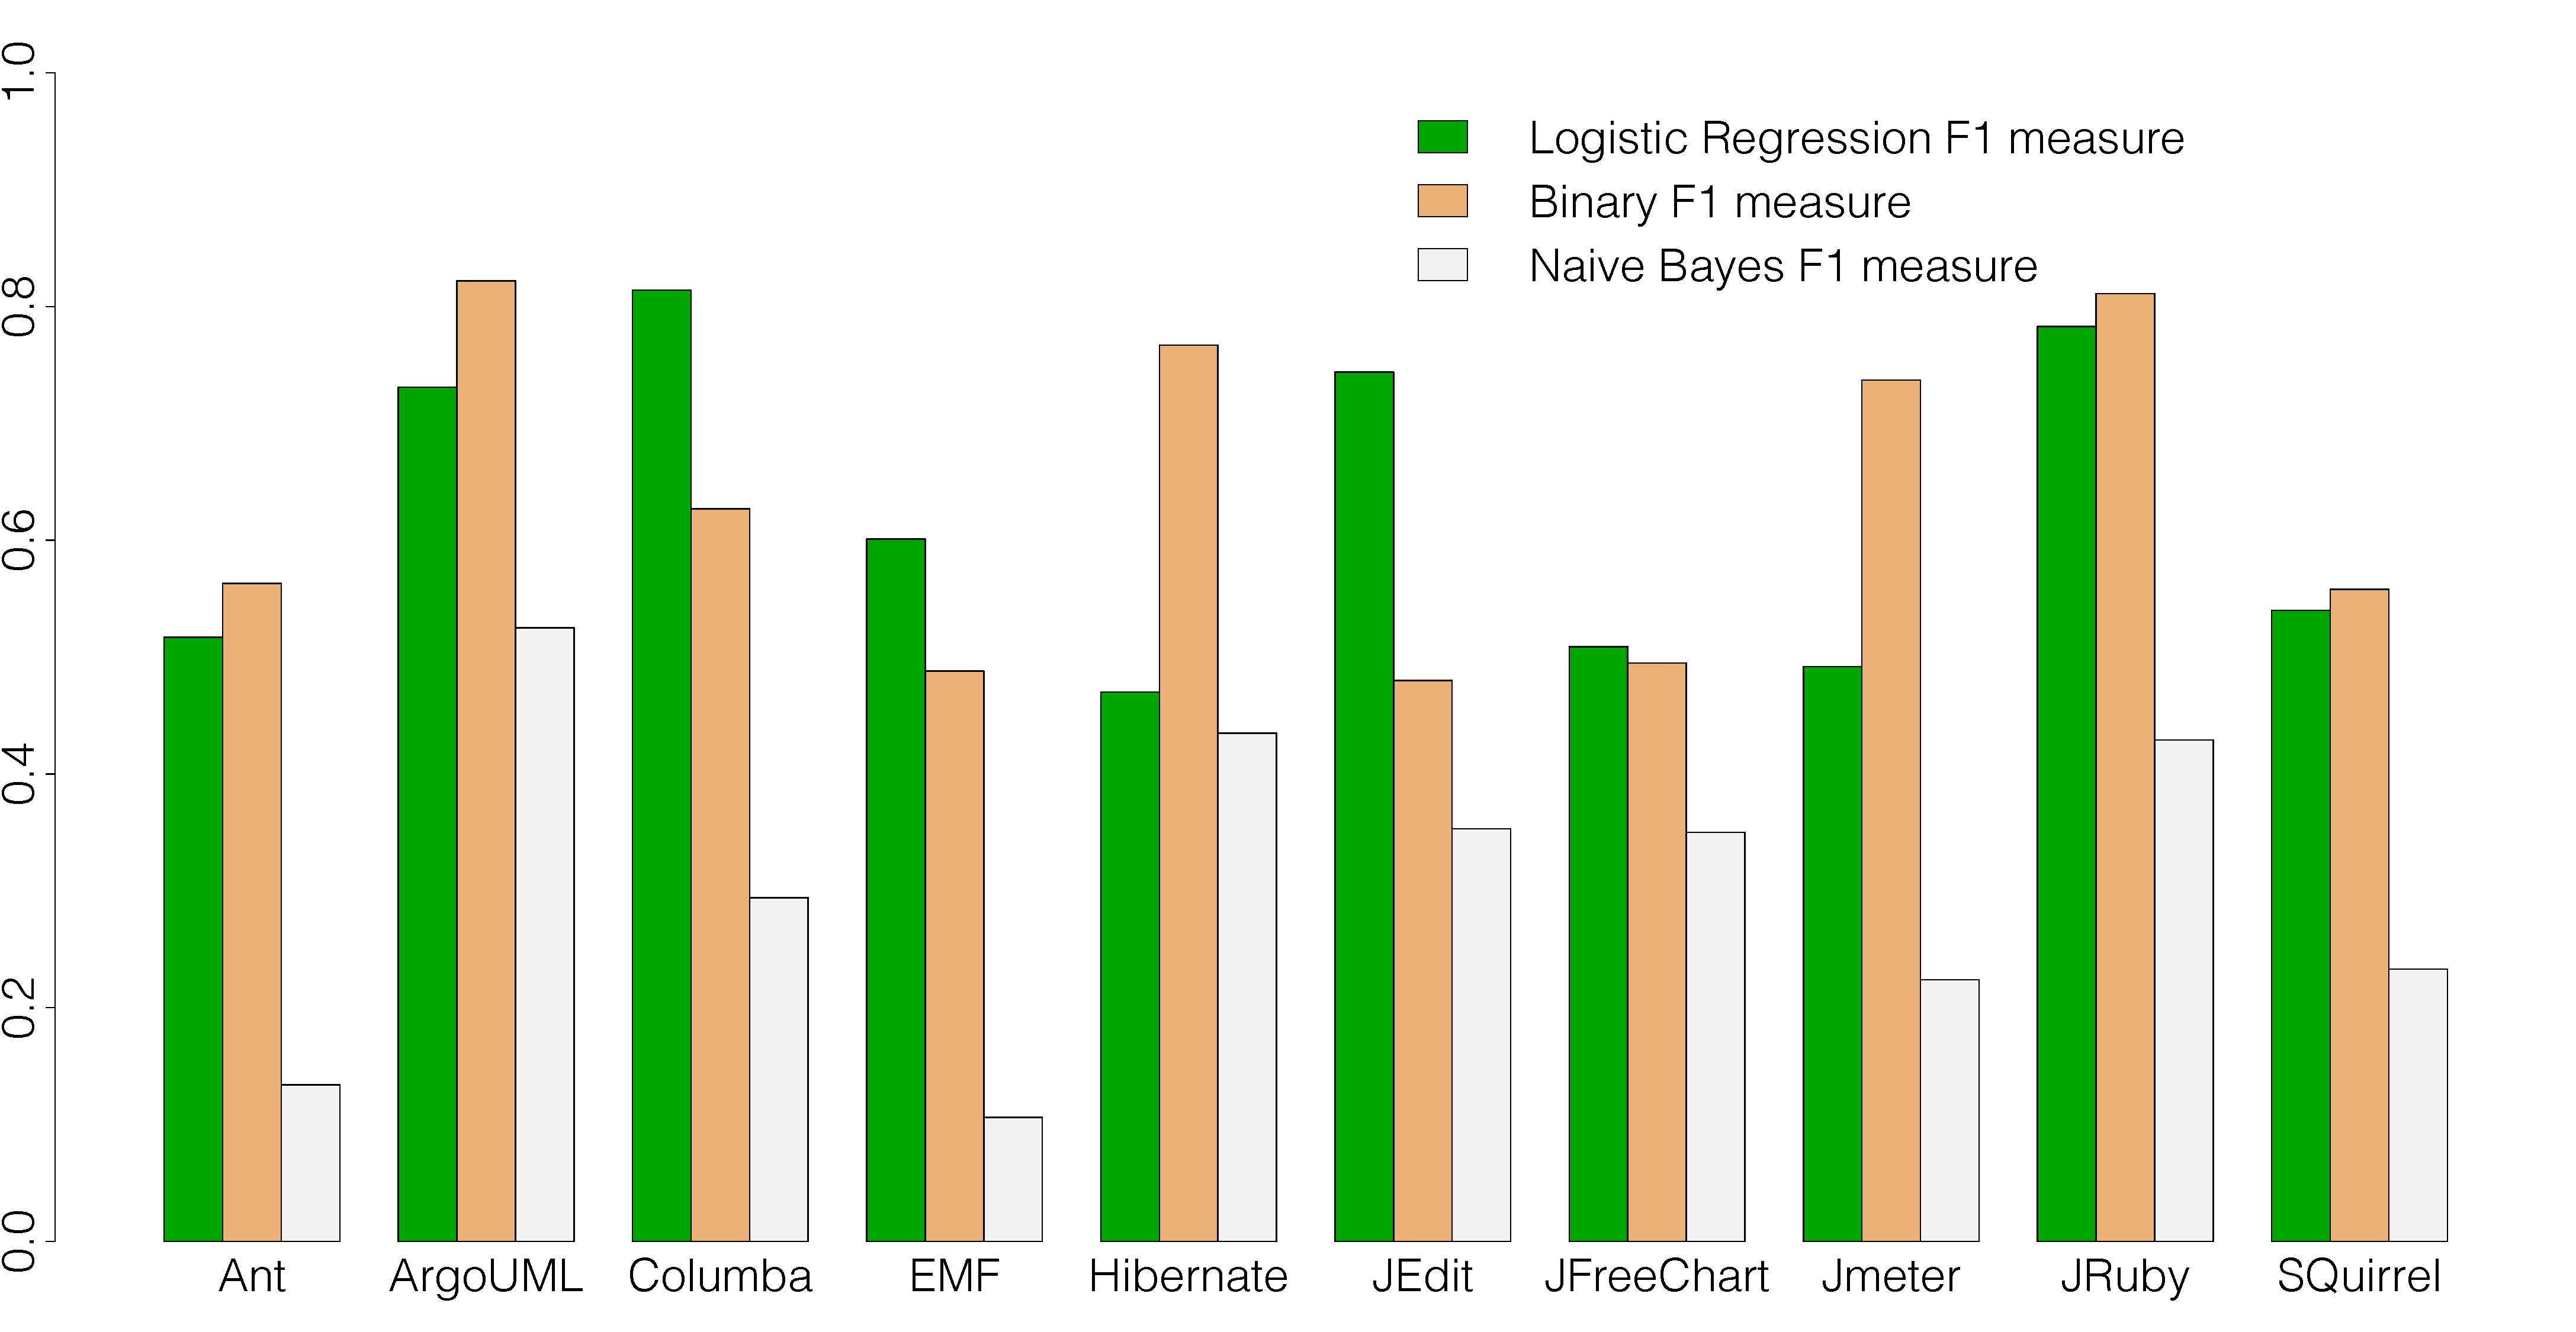
\includegraphics[width=0.48\textwidth]{figures/classifier_algorithms_comparison_design.pdf}
  \label{fig:algorithms_comparison_design}}
  \subfigure[Requirement Debt]{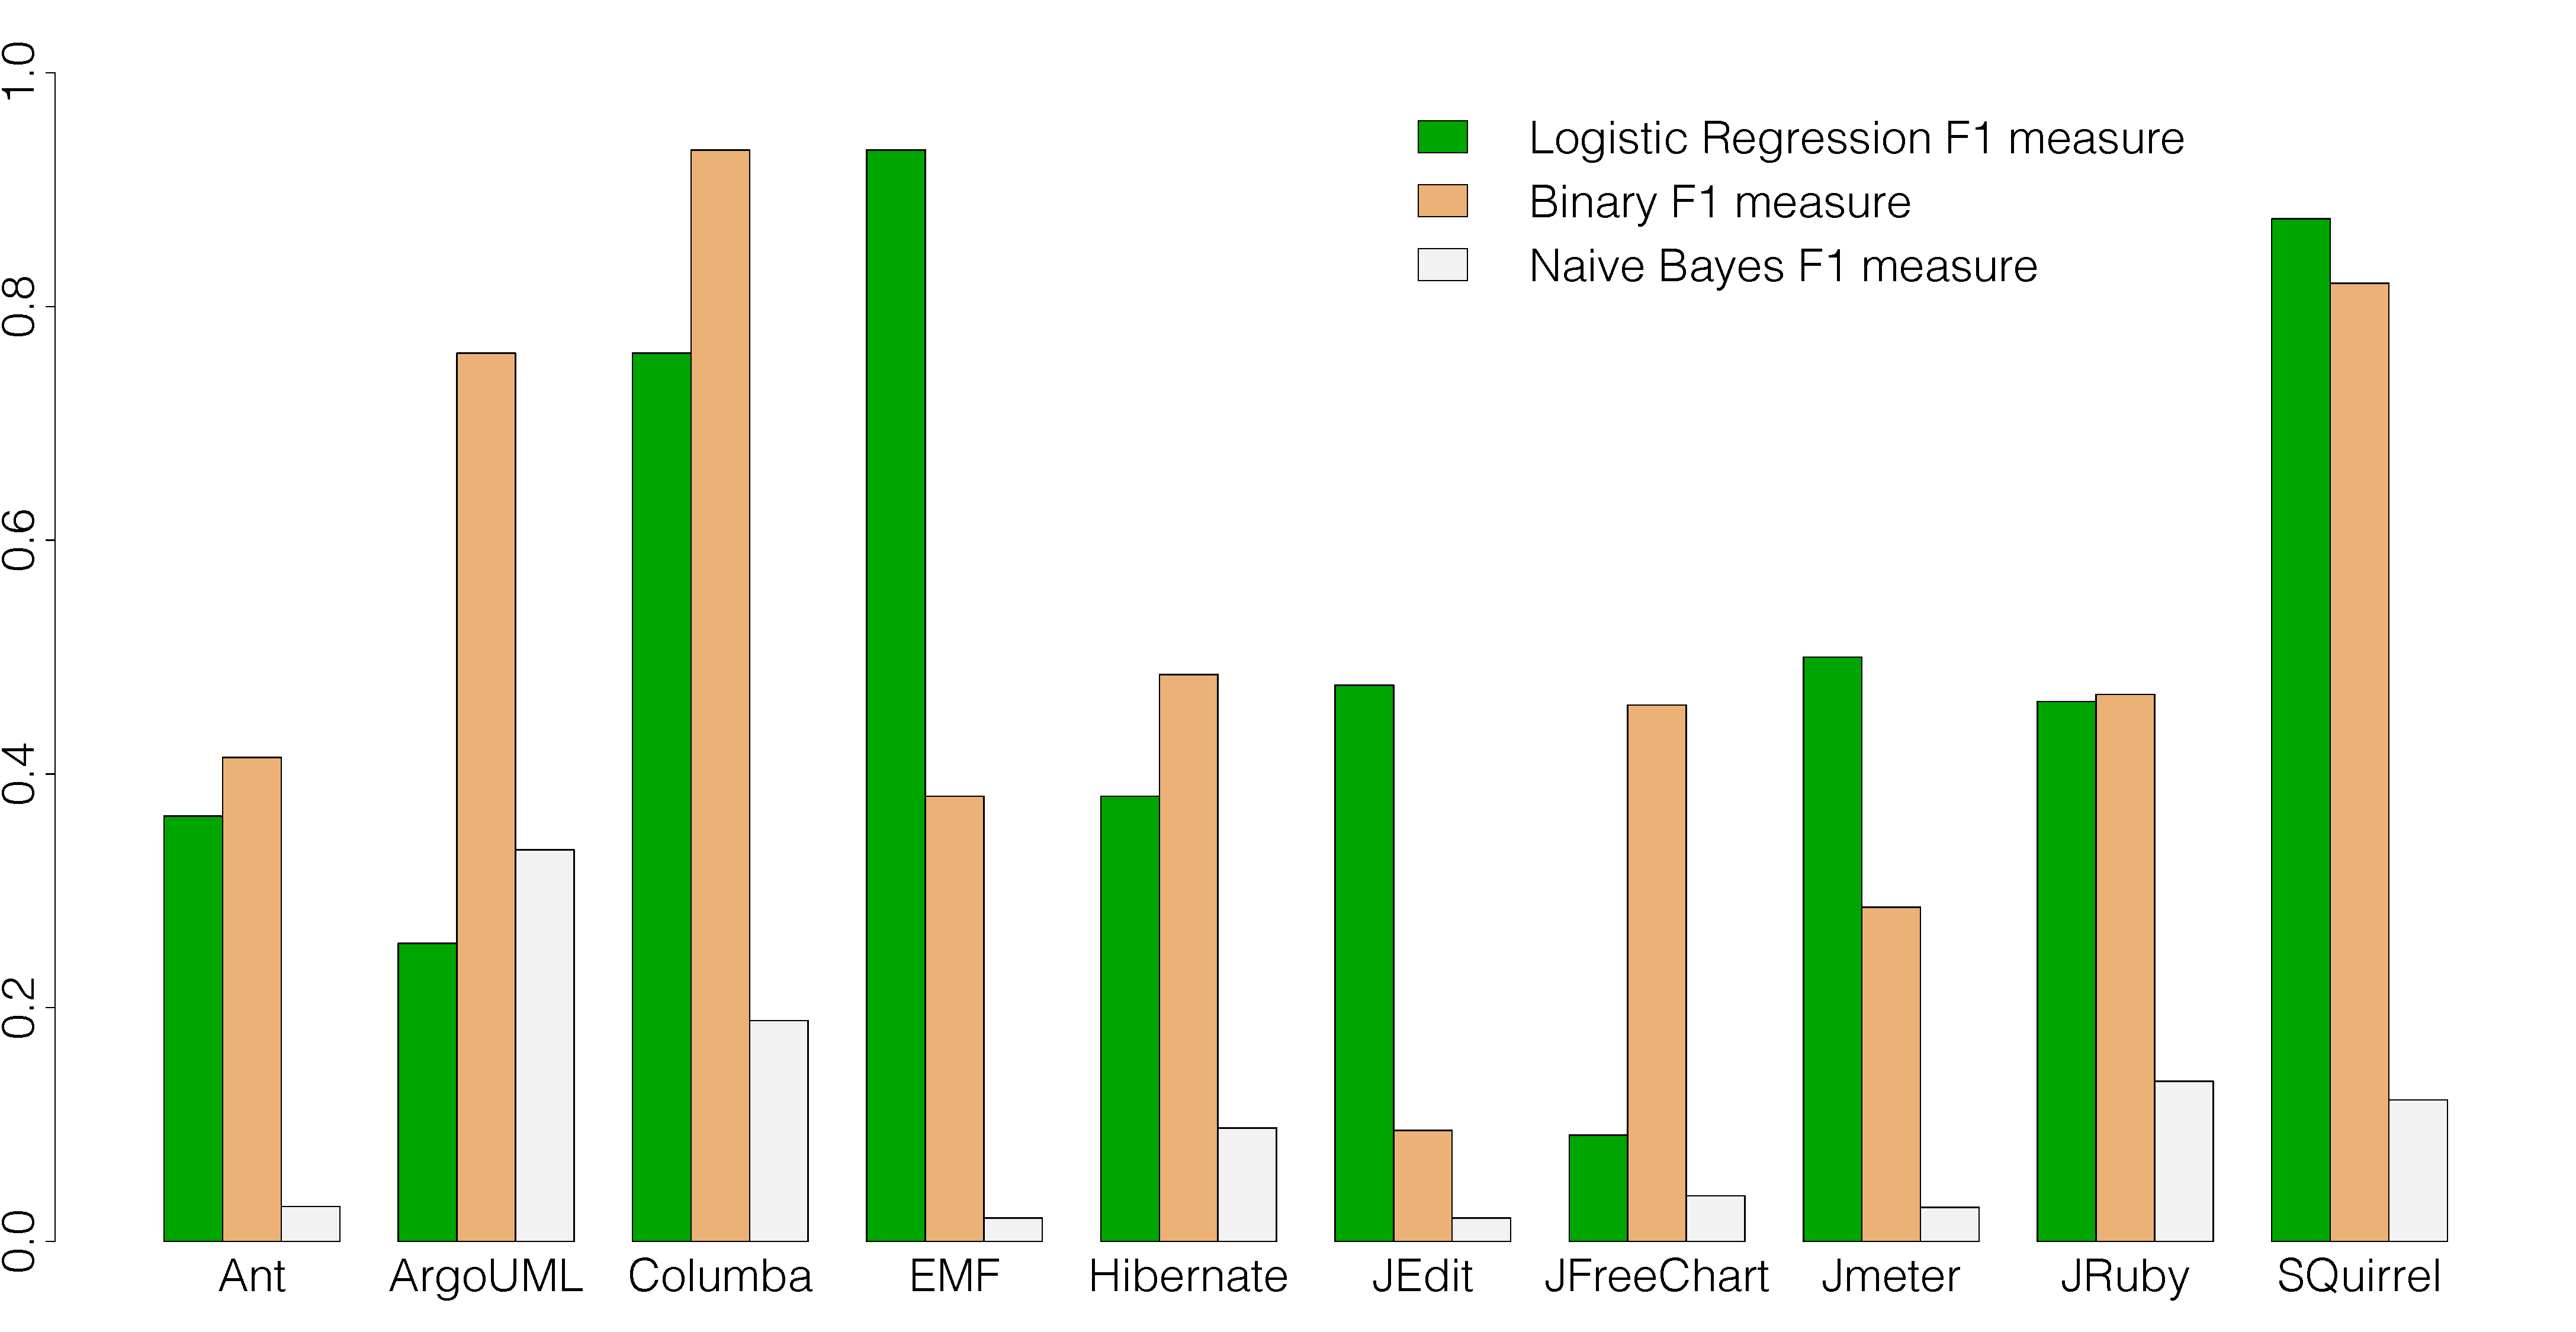
\includegraphics[width=0.48\textwidth]{figures/classifier_algorithms_comparison_requirement.pdf}
  \label{fig:algorithms_comparison_requirement}}
  \caption{Classification algorithms performance comparison}
  \label{fig:algorithms_comparison}
\end{figure*}

In this paper we propose an approach to identify \SATD comments using the Stanford Classifier. This tool, once trained correctly, can automatically classify natural language text. We create a training dataset of \SATD comments and analyzed the classification performance across ten open source projects. In RQ1, we show that our approach can outperform the current state-of-the-art in 10 out of 10 projects while identifying design and requirement debt. However, is not clear the reason why our approach was not equally effective across all projects. For example, JEdit has the worst F1 measure of all projects while classifying requirement \SATD.

\subsection{Investigating Outlier Projects}
By investigating JEdit comments, we notice two main reasons: first, the project has 10,322 comments. Of those only 14 are requirement \SATD. The data distribution represents a challenge to the classification. Even though the dataset is very unbalanced our precision was 0.125, which compared with the random classifier baseline precision of 0.001, shows that our approach is still much more useful. Second, most requirement \SATD comments in this project are in the middle of long comments. Since our approach create a high number of prediction features for \SATD comments and also for without technical debt comments, long comments have more chances to match a higher number of without technical debt features. Therefore, long comments can generate `noise' that hinders the classification performance. One possible way to reduce this effect is through the addition of more similar data, as the addition of more similar data can change the prediction features generated by the classifier. 

\emad{I do not see the point of the 2 paragraphs below}

\emad{begin: remove} Intuitively we know that each project has its own particularities, and that each group of developers, must often, create a unique way to communicate their concerns with each other. This unique trait of source code comments is inherited from the natural language itself and renders the fully automated prediction of every single \SATD very unlikely. Even when analyzing a old aged project, changes in the context of the application and turnover of developers can reflect changes in the way that source code comments are written. We can notice the impact of these particularities on the detailed performance analysis conducted in RQ3, where we can notice that the addition of more comments can eventually decrease the F1 measure performance.


For a great portion of \SATD comments there are common traits. Words as `workaround', `hack' are commonly imbued with criticism and the developers sense that this is not the appropriate solution for the problem in hand. However, relying just in these words for the identification of \SATD is not good enough as shown in Figures \ref{fig:f1_measure_comparison_design_debt} and \ref{fig:f1_measure_comparison_requirement_debt}. Therefore, NLP techniques, as proposed in our work, are needed in order to effectively identify \SATD comments.
\emad{end: remove}

\subsection{Investigating the Impact of the Underlying Classifier of the NLP Classification}

In our work, all the classification done by the Stanford Classifier used a Logistic Regression classifier. However, would be interesting to see how other  algorithms perform when classifying our dataset. Then, we choose two other algorithms to execute the classification with: Naive Bayes generative classifier and Binary classifier.

Figures \ref{fig:algorithms_comparison_design} and \ref{fig:algorithms_comparison_requirement} compare the performance between the three different algorithms. We find that the Naive Bayes has the eorst average F1-measure of 0.308 and 0.058 for design and requirement technical debt, respectively. The reason behind the low F1-measure average is that the Naive Bayes algorithm favors recall at the expense of precision \emad{we need a citation for this claim}. For example, while classifying design debt, the average recall was of 0.847 and precision 0.195. The two other algorithms present more balanced results compared to Naive Bayes, and the difference in performance between them is not as accentuate. The Logistic Regression classifier achieved F1-measures of 0.620 and 0.403, while the binary classifier F1-measures for design and requirement \SATD is 0.634 and 0.400, respectively. 

Although the Binary classification has a slightly better performance, for our research purpose, the Logistical Regression algorithm provide more insightful features as outcome. These features were analyzed and presented in RQ2. 

\subsection{Textual Similarity for Design and Requirement Debt}

\section{Related Work}
\label{sec:related_work}
% -*- root: main.tex -*-
Our work uses code comments to detect \SATD using a Natural Language Processing (NLP) technique. Therefore, we divide the related work into three subsections, namely source code comments, technical debt, and NLP in Software Engineering.

\subsection{Source Code Comments}

A number of studies examined the co-evolution of source code comments and the rationale for changing code comments. For example, Fluri \textit{et al.}~\cite{Fluri2007WCRE} analyzed the co-evolution of source code and code comments, and found that 97\% of the comment changes are consistent. Tan \textit{et al.}~\cite{Tan2012ICST} proposed a novel approach to identify inconsistencies between Javadoc comments and method signatures. Malik \textit{et al.} \cite{Malik2008ICSM} studied the likelihood of a comment to be updated and found that call dependencies, control statements, the age of the function containing the comment, and the number of co-changed dependent functions are the most important factors to predict comment updates.

Other works used code comments to understand developer tasks. For example. Storey \textit{et al.}~\cite{Storey2008ICSE} analyzed how task annotations (e.g., TODO, FIXME) play a role in improving team articulation and communication. The work closest to ours is the work by Potdar and Shihab~\cite{Potdar2014ICSME}, where code comments were used to identify technical debt, called \SATD. 

Similar to some of the prior work, we also use source code comments to identify technical debt. However, our main focus is on the detection of different \emph{types} of \SATD. As we have shown, our approach yields different and better results in the detection of \SATD.
%Furthermore, we propose an approach to identify \SATD, that is derived from source code comments and natural language processing techniques, to detect \SATD.

\subsection{Technical Debt}

A number of studies has focused on the detection and management of technical debt. For example, Seaman \textit{et al.}~\cite{Seaman2011}, Kruchten \textit{et al.}~\cite{Kruchten2013IWMTD} and Brown \textit{et al.}~\cite{Brown2010MTD} make several reflections about the term technical debt and how it has been used to communicate the issues that developers find in the code in a way that managers can understand. 

Other work focused on the detection of technical debt. Zazworka \textit{et al.} \cite{Zazworka2013CSE} conducted an experiment to compare the efficiency of automated tools in comparison with human elicitation regarding the detection of technical debt. They found that there is a small overlap between the two approaches, and thus it is better to combine them than replace one with the other. In addition, they concluded that automated tools are more efficient in finding defect debt, whereas developers can realize more abstract categories of technical debt.

In a follow up work, Zazworka \textit{et al.}~\cite{Zazworka2011MTD} conducted a study to measure the impact of technical debt on software quality. They focused on a particular kind of design debt, namely, God Classes. They found that God Classes are more likely to change, and therefore, have a higher impact on software quality. Fontana \textit{et al.}~\cite{Fontana2012MTD} investigated design technical debt appearing in the form of code smells. They used metrics to find three different code smells, namely God Classes, Data Classes and Duplicated Code. They proposed an approach to classify which one of the different code smells should be addressed first, based on its risk. Ernst \textit{et al.} ~\cite{Ernst2015FSE} conducted a survey with 1,831 participants and found that architectural decisions are the most important source of technical debt.

Our work is different from the work that uses code smells to detect design technical debt, since we use code comments to detect technical debt. Moreover, our approach does not rely on code metrics and thresholds to identify technical debt and can be used to identify bad quality code symptoms other than bad smells.

More recently, Potdar and Shihab~\cite{Potdar2014ICSME} extracted the comments of four projects and analyzed 101,762 comments to come up with 62  patterns that indicate self-admitted technical debt. Their findings show that 2.4\% - 31\% of the files in a project contain self-admitted technical debt. Our earlier work ~\cite{Maldonado2015MTD} examined more than 33 thousands comments to classify the different types of \SATD found in source code comments. Farias \textit{et al.} ~\cite{Farias2015MTD} proposed a contextualized vocabulary model for identifying technical debt in comments using word classes and code tags in the process. 

Our work also uses code comments to detect design technical debt. However, we use these code comments to train a \revised{maximum entropy classifier}{R2-11} to automatically identify technical debt. Also, our focus is on \emph{self-admitted} design and requirement technical debt.

\subsection{NLP in Software Engineering}

A number of studies leveraged NLP in software engineering, mainly for the traceability of requirements, program comprehension and software maintenance. For example, Lormans and van Deursen~\cite{Lormans2006CSRM} used latent semantic indexing (LSI) to create traceable links between requirements and test cases and requirements to design implementations. Hayes \textit{et al.}~\cite{Hayes2005, Hayes2006TSE} created a tool called RETRO that applies information retrieval techniques to trace and map requirements to designs. Yadla \textit{et al.}~\cite{yadla2005tracing} further enhanced the RETRO tool and linked requirements to issue reports. On the other hand, Runeson \textit{et al.}~\cite{Runeson2007ICSE} implemented a NLP-based tool to automatically identify duplicated issue reports, they found that 2/3 of the possible duplicates examined in their study can be found with their tool. Canfora and Cerulo \cite{Canfora2005ISSM} linked a change request with the corresponding set of source files using NLP techniques, and then, they evaluated the performance of the approach on four open source projects.  

The prior work motivated us to use NLP techniques. However, our work is different from the aforementioned ones, since we apply NLP techniques on code comments to identify \SATD, rather than use it for traceability and linking between different software artifacts.

\section{Conclusion and Future work}
\label{sec:conclusion}
Technical debt is a term being used to express non optimal solutions, such as hacks and workarounds, that are applied during the software development process. Although these non optimal solutions can provide a way to achieve immediate pressing goals, most often they will have a negative impact in the project maintainability, and will require an increased effort to be properly addressed in the long run. 

Our work focuses in the identification of \SATD through the use of Natural Processing Language. \SATD is the technical debt deliberately introduced by the developers and reported through source code comments.

We analyzed the comments of 10 open source projects namely Apache Ant, Apache Jmeter, ArgoUML, Columba, EMF, Hibernate, JEdit, JFreeChart, JRuby and SQuirrel. These projects are considered well commented and they belong to different application domains.

The comments of these projects where manually classified into specif types of technical debt such as design, requirement, defect, documentation and test debt. This dataset with more than 63,000 of classified comments were used to create training datasets to a maximum entropy classifier tool and then used to identify  design and requirement \SATD.

We find that our approach is 2 to 20 times more efficient in the identification of \SATD than the state-of-the-art approach. We achieved an average F1 measure of 0.62 and 0.51 while identifying design and requirement \SATD comments respectively. 

We analyzed strong indicators of \SATD in code comments and we ranked the top 10 words used by developers to express design and requirement debt in the studied projects. For design debt the most common indicators were `hack', `workaround', `kludge', `yuck!', `fixme', `todo', `stupidity', `ugly', `unused?' and `sucks'. Whereas, for requirement debt the most common words were: `todo', `needed', `implementation', `fixme', `xxx', `auto-generated', `ends?', `configurable', `convention' and `apparently'.
 
Regarding the amount of data necessary to effectively identify \SATD comments using our approach we find that training datasets with at least 1,444 design debt comments can be used to identify \SATD. Similarly, datasets with at least 1,055 requirement debt comments can be used for the purpose of requirement \SATD identification. 

In this work, we contribute with the dataset created in this study making it publicly available, we believe that it will be a good starting point for researchers interested in identifying technical debt through comments and even using different types of Natural Processing Language techniques. 

In a future work we will use the findings of this study to build a tool that will support software engineers in the task of identifying and managing the \SATD portfolio. We believe that our dataset can be used towards the effective identification of \SATD comments and it will be beneficial to the developer to see technical debt that was pointed out by other humans instead of relying in metrics and thresholds. 

\bibliographystyle{abbrv}
\bibliography{bibliography}  


\appendix{}
\label{sec:appendix}

\subsection*{Detailed Precision and Recall Values}

In Section~\ref{sec:case_study_results}, we presented the F1-measures for all projects when answering our RQs. In this appendix, we added the detailed precision and recall values that make up the F1-measures.


\begin{table*}[h!]
    \begin{center}
        \caption{Detailed Comparison of F1-measure Between the NLP-based, the Comment Patterns and the Random Baseline Approaches for Design Debt}
        \label{tbl:classifier_results_vs_baseline_design}
        \begin{tabular}{l| c c c|| c c c|| c c c}
        \toprule

        \multirow{4}{*}{\textbf{\thead{Project}}} & \multicolumn{3}{c||}{\textbf{\thead{NLP-based}}} & \multicolumn{3}{c||}{\textbf{\thead{Comment Patterns}}} & \multicolumn{3}{c}{\textbf{\thead{Random Baseline}}} 
        
        \\ 
        \cmidrule{2-10}
        
        & \textbf{\thead{Precision}} & \textbf{\thead{Recall}} & \textbf{\thead{F1 measure}} & \textbf{\thead{Precision}} & \textbf{\thead{Recall}} & \textbf{\thead{F1 measure}} & \textbf{\thead{Precision}} & \textbf{\thead{Recall}} & \textbf{\thead{F1 measure}}\\
        \midrule
        \textbf{Ant}           &   0.554 &   0.484 &  0.517 &   0.526 &  0.105 &    0.175 &  0.024 & 0.5 & 0.045 \\
        \textbf{ArgoUML}       &   0.788 &   0.843 &  0.814 &   0.786 &  0.041 &    0.078 &  0.092 & 0.5 & 0.155 \\
        \textbf{Columba}       &   0.792 &   0.484 &  0.601 &   0.833 &  0.079 &    0.145 &   0.02 & 0.5 & 0.038 \\
        \textbf{EMF}           &   0.574 &   0.397 &  0.470 &     0.5 &  0.064 &    0.114 &  0.018 & 0.5 & 0.035 \\
        \textbf{Hibernate}     &   0.877 &   0.645 &  0.744 &   0.906 &  0.082 &     0.15 &  0.136 & 0.5 & 0.214 \\
        \textbf{JEdit}         &   0.779 &   0.378 &  0.509 &   0.867 &  0.199 &    0.324 &  0.019 & 0.5 & 0.037 \\
        \textbf{JFreeChart}    &   0.646 &   0.397 &  0.492 &   0.833 &  0.027 &    0.053 &  0.043 & 0.5 &  0.08 \\
        \textbf{Jmeter}        &   0.808 &   0.668 &  0.731 &   0.733 &   0.07 &    0.127 &   0.04 & 0.5 & 0.075 \\
        \textbf{JRuby}         &   0.798 &   0.770 &  0.783 &   0.765 &  0.076 &    0.138 &  0.075 & 0.5 & 0.131 \\
        \textbf{SQuirrel}      &   0.544 &   0.536 &  0.540 &   0.471 &  0.038 &    0.071 &   0.03 & 0.5 & 0.056 \\
        \bottomrule
        \end{tabular}
    \end{center}    
\end{table*}
                 

\begin{table*}
    \begin{center}
        \caption{Detailed Comparison of F1-measure Between the NLP-based, the Comment Patterns and the Random Baseline Approaches for Requirement Debt}
        \label{tbl:classifier_results_vs_baseline_requirement}
        \begin{tabular}{l| c c c|| c c c|| c c c}
        \toprule

        \multirow{4}{*}{\textbf{\thead{Project}}} & \multicolumn{3}{c||}{\textbf{\thead{NLP-based}}} & \multicolumn{3}{c||}{\textbf{\thead{Comment Patterns}}} & \multicolumn{3}{c}{\textbf{\thead{Random Baseline}}} 
        
        \\ 
        \cmidrule{2-10}
        
        & \textbf{\thead{Precision}} & \textbf{\thead{Recall}} & \textbf{\thead{F1 measure}} & \textbf{\thead{Precision}} & \textbf{\thead{Recall}} & \textbf{\thead{F1 measure}} & \textbf{\thead{Precision}} & \textbf{\thead{Recall}} & \textbf{\thead{F1 measure}}\\
        \midrule
        \textbf{Ant}           &  0.154 & 0.154 &  0.154 & 0.0 & 0.0 & 0.0 & 0.003 &  0.5 &  0.006 \\
        \textbf{ArgoUML}       &  0.663 & 0.540 &  0.595 & 0.0 & 0.0 & 0.0 & 0.045 &  0.5 &  0.083 \\
        \textbf{Columba}       &  0.755 & 0.860 &  0.804 & 0.0 & 0.0 & 0.0 & 0.007 &  0.5 &  0.013 \\
        \textbf{EMF}           &  0.800 & 0.250 &  0.381 & 0.0 & 0.0 & 0.0 & 0.004 &  0.5 &  0.007 \\
        \textbf{Hibernate}     &  0.610 & 0.391 &  0.476 & 0.0 & 0.0 & 0.0 & 0.022 &  0.5 &  0.042 \\
        \textbf{JEdit}         &  0.125 & 0.071 &  0.091 & 0.0 & 0.0 & 0.0 & 0.001 &  0.5 &  0.003 \\
        \textbf{JFreeChart}    &  0.220 & 0.600 &  0.321 & 0.0 & 0.0 & 0.0 & 0.003 &  0.5 &  0.007 \\
        \textbf{Jmeter}        &  0.153 & 0.524 &  0.237 & 0.0 & 0.0 & 0.0 & 0.003 &  0.5 &  0.005 \\
        \textbf{JRuby}         &  0.686 & 0.318 &  0.435 & 0.0 & 0.0 & 0.0 & 0.023 &  0.5 &  0.044 \\
        \textbf{SQuirrel}      &  0.657 & 0.460 &  0.541 & 0.0 & 0.0 & 0.0 & 0.007 &  0.5 &  0.014 \\
        \bottomrule
        \end{tabular}
    \end{center}    
\end{table*}

% \clearpage

% \begin{table}
%     \begin{center}
%         \caption{Technical Debt distribution per type}
%         \label{tbl:td_distribution}
%         \begin{tabular}{l|ccccccc}
%         \toprule
%         \multirow{2}{*}{Project} & \multicolumn{3}{c}{TD Distribution} \\ & {Design} & {Req.}  & {Other} & \multirow{-2}{*}{Total TD comments} & \multirow{-2}{*}{Total comments} &  \multirow{-2}{*}{TD \%} \\
%         \midrule
%         Ant            &  95 &  13  &  23 &   131 &   4,137  & 03.1 \\
%         ArgoUML        &  801 & 411 & 201 & 1.413 &   9,548  & 14.7 \\
%         Columba        &  126 &  43 &  35 &   204 &   6,478  & 03.1 \\
%         EMF            &  78 &  16  &  10 &   104 &   4,401  & 02.3 \\
%         Hibernate      &  355 &  64 &  53 &   472 &   2,968  & 15.9 \\
%         JEdit          &  196 &  14 &  46 &   256 &  10,322  & 02.4 \\
%         JFreeChart     &  184 &  15 &  10 &   209 &   4,423  & 04.7 \\
%         Jmeter         &  316 &  21 &  37 &   374 &   8,162  & 04.5 \\
%         JRuby          &  343 & 110 & 169 &   622 &   4,897  & 12.7 \\
%         SQuirrel       &  209 & 50  & 27  &   286 &   7,230  & 03.9 \\
%         \bottomrule
%         \end{tabular}
%     \end{center}    
% \end{table}



% \clearpage

% \begin{table}[!hbt]
%     \begin{center}
%         \caption{Design Debt features per project}
%         \label{tbl:design_features_per_project}
%         \begin{tabular}{l| c c c }
%         \toprule
%         \textbf{Project} & \thead{Positive\\Design TD\\Features} & \thead{Negative\\Design TD\\Features} & \thead{Total\\Features} \\
%         \midrule
%         Ant          &5,299 & 23,623 &28,922 \\
%         ArgoUML      &3,917 & 26,012 &29,929 \\
%         Columba      &5,255 & 24,182 &29,437 \\
%         EMF          &5,346 & 23,667 &29,013 \\
%         Hibernate    &4,914 & 24,070 &28,984 \\
%         JEdit        &5,042 & 24,644 &29,686 \\
%         JFreeChart   &5,361 & 23,530 &28,891 \\
%         Jmeter       &5,172 & 23,916 &29,088 \\
%         JRuby        &4,856 & 24,553 &29,409 \\
%         SQuirrel     &4,982 & 25,146 &30,128 \\
%         \midrule
%         Average       & 5,014  & 24,334 & 29,348  \\      
%         Total unique  & 6,327  & 31,518 & 35,828  \\
%         \bottomrule
%         \end{tabular}
%     \end{center}    
% \end{table}

% \begin{table}[!hbt]
%     \begin{center}
%         \caption{Requirement Debt features per project}
%         \label{tbl:requirement_features_per_project}
%         \begin{tabular}{l| c c c }
%         \toprule
%         \textbf{Project} & \thead{Requirement TD\\features} & \thead{No TD\\Features} & \thead{Total\\Features} \\
%         \midrule
%         Ant           & 1,812 & 27,673 & 29,485  \\
%         ArgoUML       & 2,779 & 27,260 & 30,039  \\
%         Columba       & 2,433 & 27,561 & 29,994  \\
%         EMF           & 1,889 & 27,637 & 29,526  \\
%         Hibernate     & 2,748 & 26,654 & 29,402  \\
%         JEdit         & 1,831 & 28,267 & 30,098  \\
%         JFreeChart    & 1,902 & 27,439 & 29,341  \\
%         Jmeter        & 1,893 & 27,716 & 29,609  \\
%         JRuby         & 2,850 & 27,085 & 29,935  \\
%         SQuirrel      & 1,814 & 26,914 & 28,728  \\
%         \midrule
%         Average       & 2,195  & 27,420 & 29,615 \\      
%         Total unique  & 4,015  & 32,954 & 32,954 \\
%         \bottomrule
%         \end{tabular}
%     \end{center}    
% \end{table}

\clearpage

\subsection*{Investigating the Amount of Training Data Required vs. Classification Performance}

In Section~\ref{sec:case_study_results} (RQ3), we presented the Figures for Ant and ArogUML only. Here, we present the same Figures for all projects, for both, design and requirement \SATD.


\begin{figure}[thb!]
  \centering
  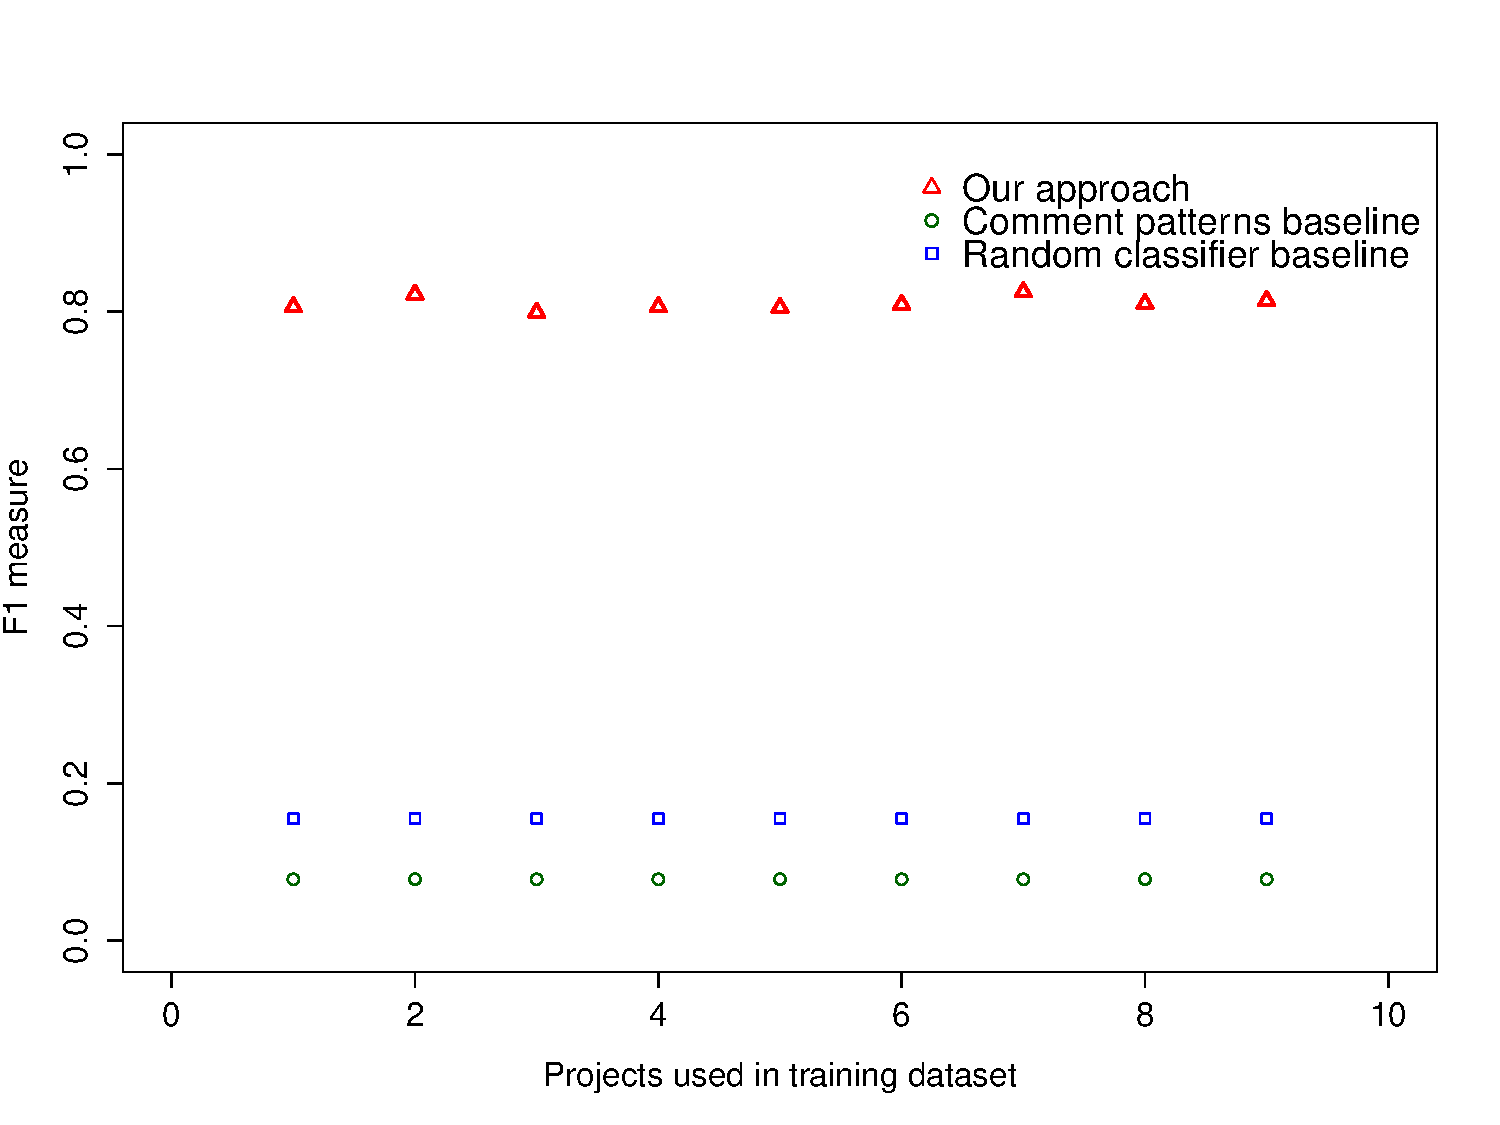
\includegraphics[width=0.49\textwidth]{figures/appendix/iteration_details/design_argo.pdf}
  % \vspace{-3mm}
  \caption{Argo Design Debt Classification}
  \label{fig:design_argo}
\end{figure}

\begin{figure}[thb!]
  \centering
  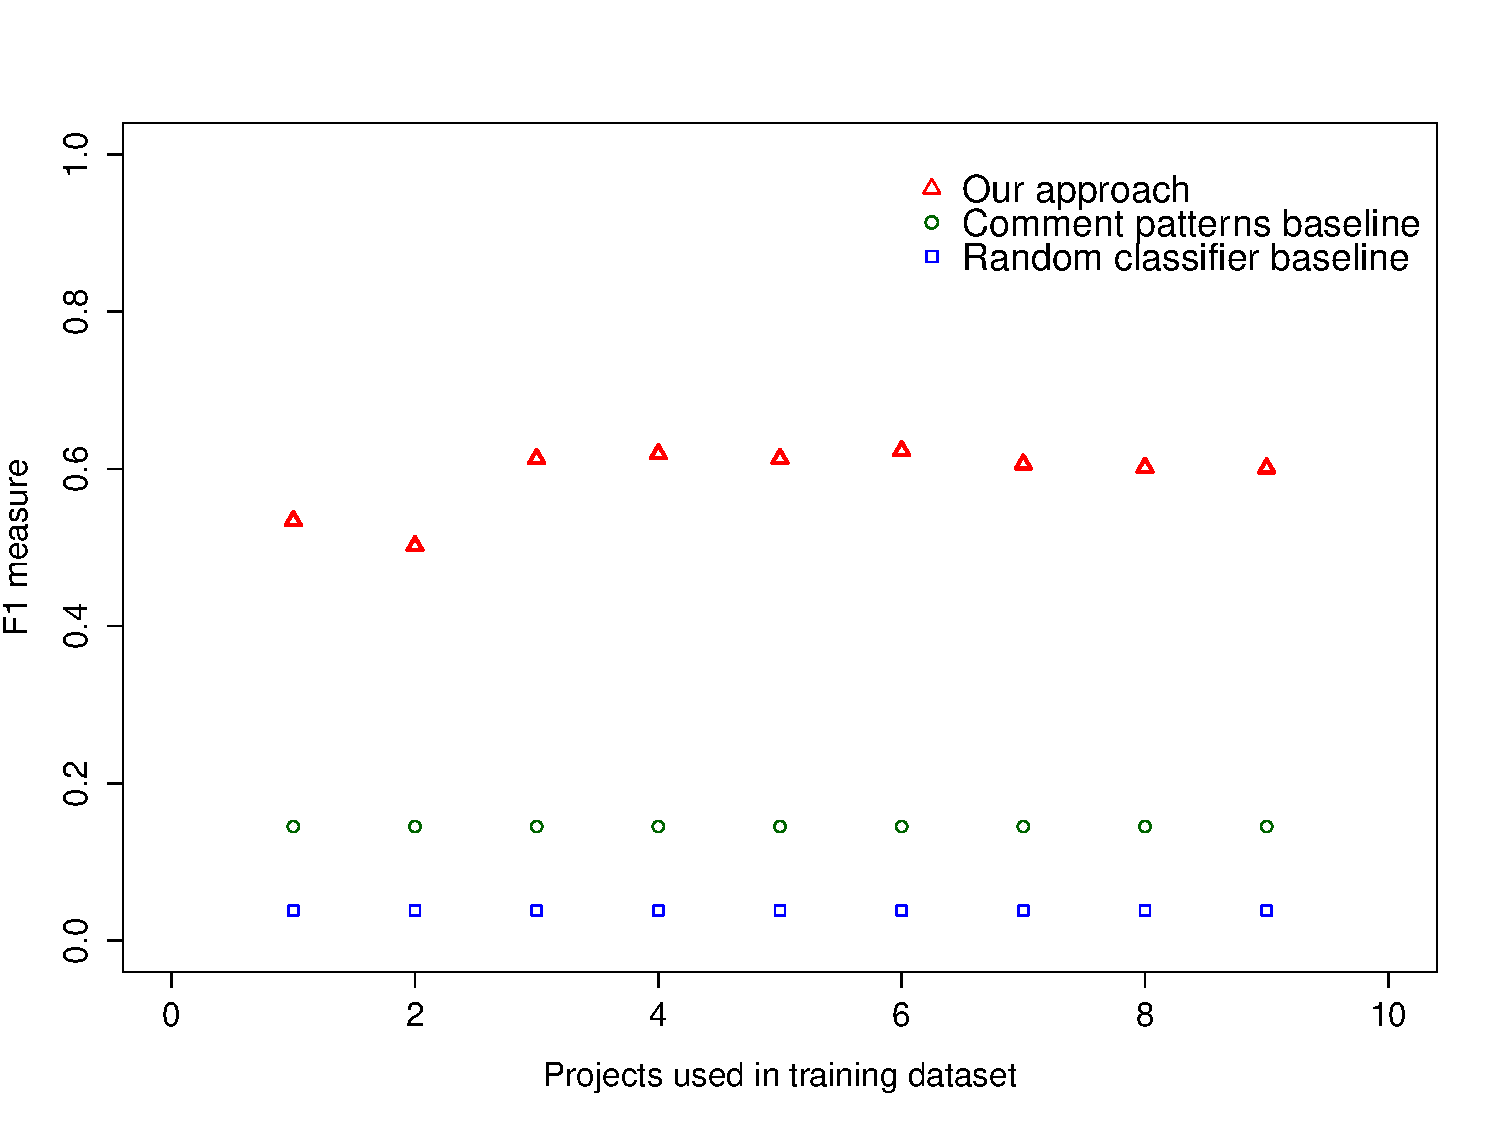
\includegraphics[width=0.49\textwidth]{figures/appendix/iteration_details/design_columba.pdf}
  % \vspace{-3mm}
  \caption{Columba Design Debt Classification}
  \label{fig:design_columba}
\end{figure}

\begin{figure}[thb!]
  \centering
  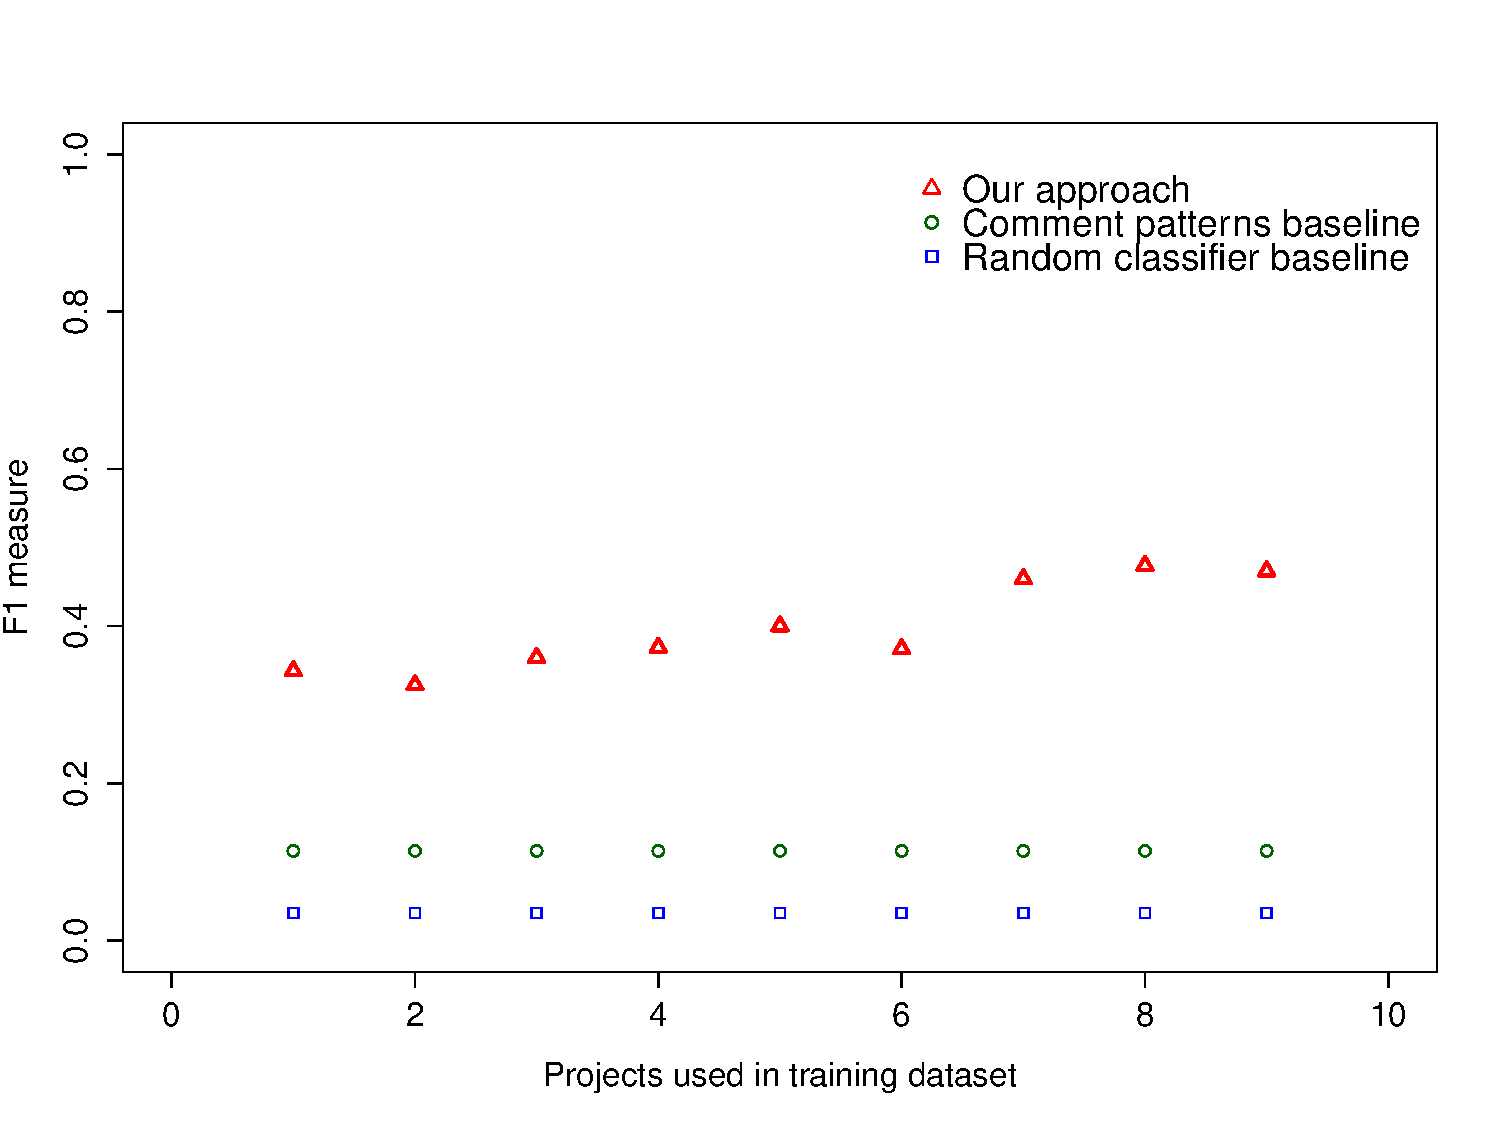
\includegraphics[width=0.49\textwidth]{figures/appendix/iteration_details/design_emf.pdf}
  % \vspace{-3mm}
  \caption{Emf Design Debt Classification}
  \label{fig:design_emf}
\end{figure}

\begin{figure}[thb!]
  \centering
  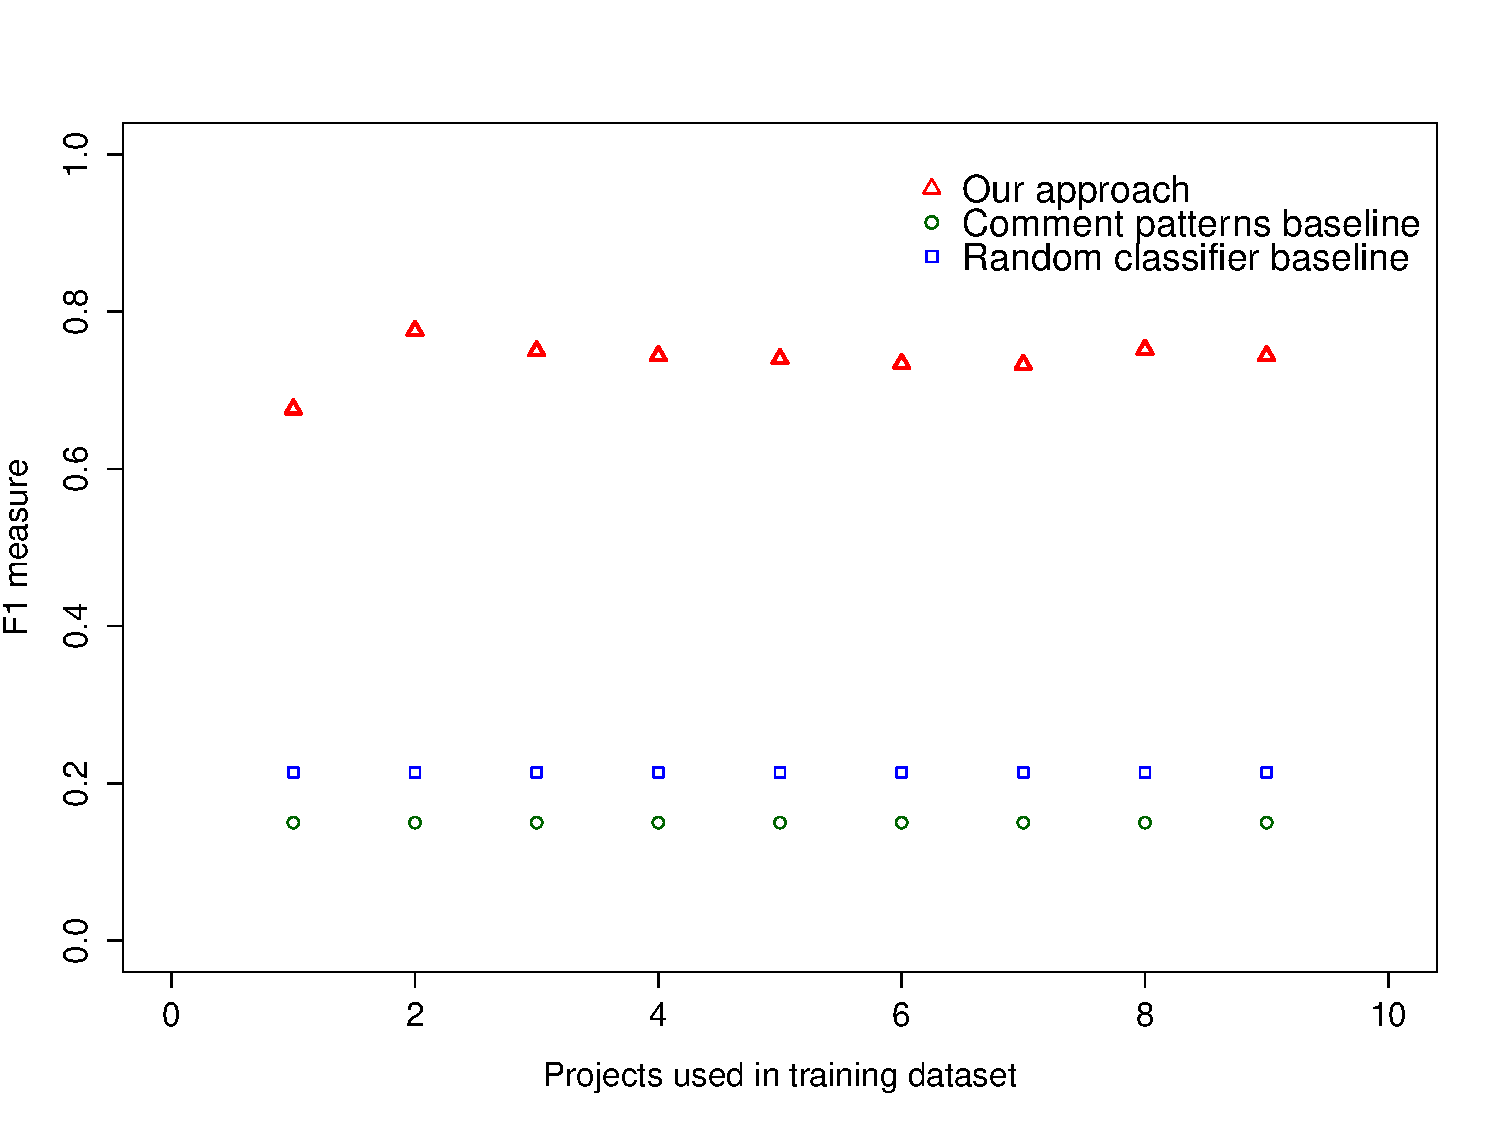
\includegraphics[width=0.49\textwidth]{figures/appendix/iteration_details/design_hibernate.pdf}
  \caption{Hibernate Design Debt Classification}
  \label{fig:design_hibernate}
\end{figure}

\begin{figure}[thb!]
  \centering
  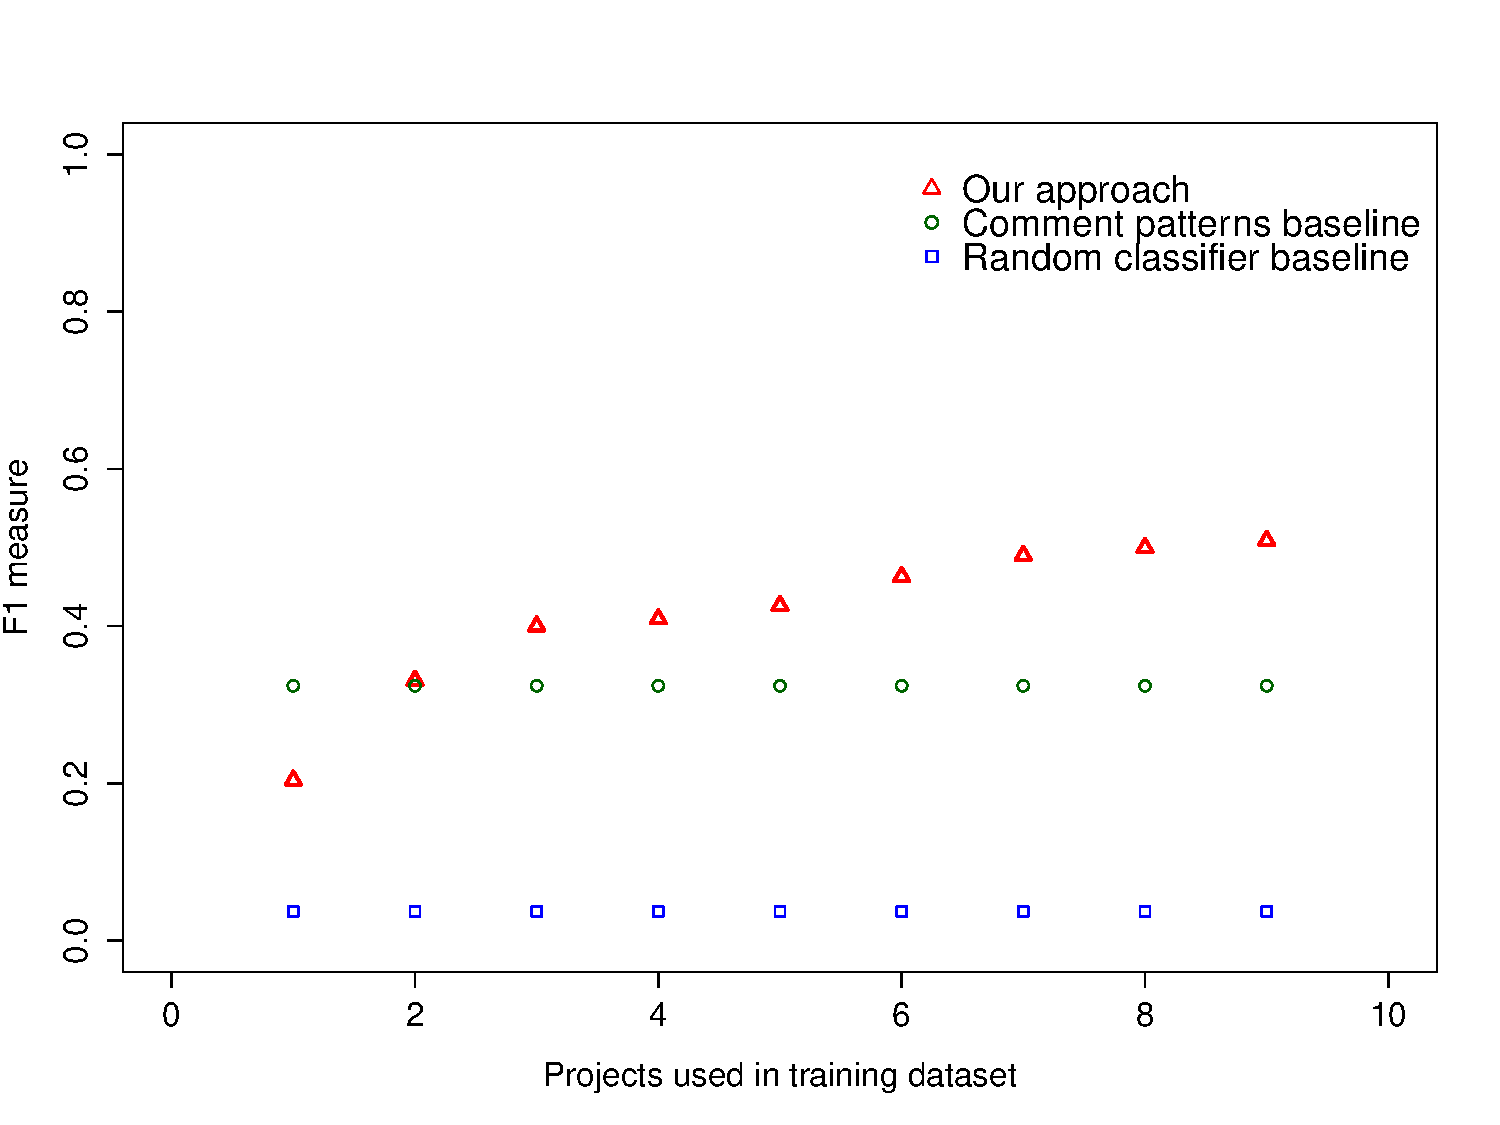
\includegraphics[width=0.49\textwidth]{figures/appendix/iteration_details/design_jedit.pdf}
  % \vspace{-3mm}
  \caption{JEdit Design Debt Classification}
  \label{fig:design_jedit}
\end{figure}

\clearpage

\begin{figure}[thb!]
  \centering
  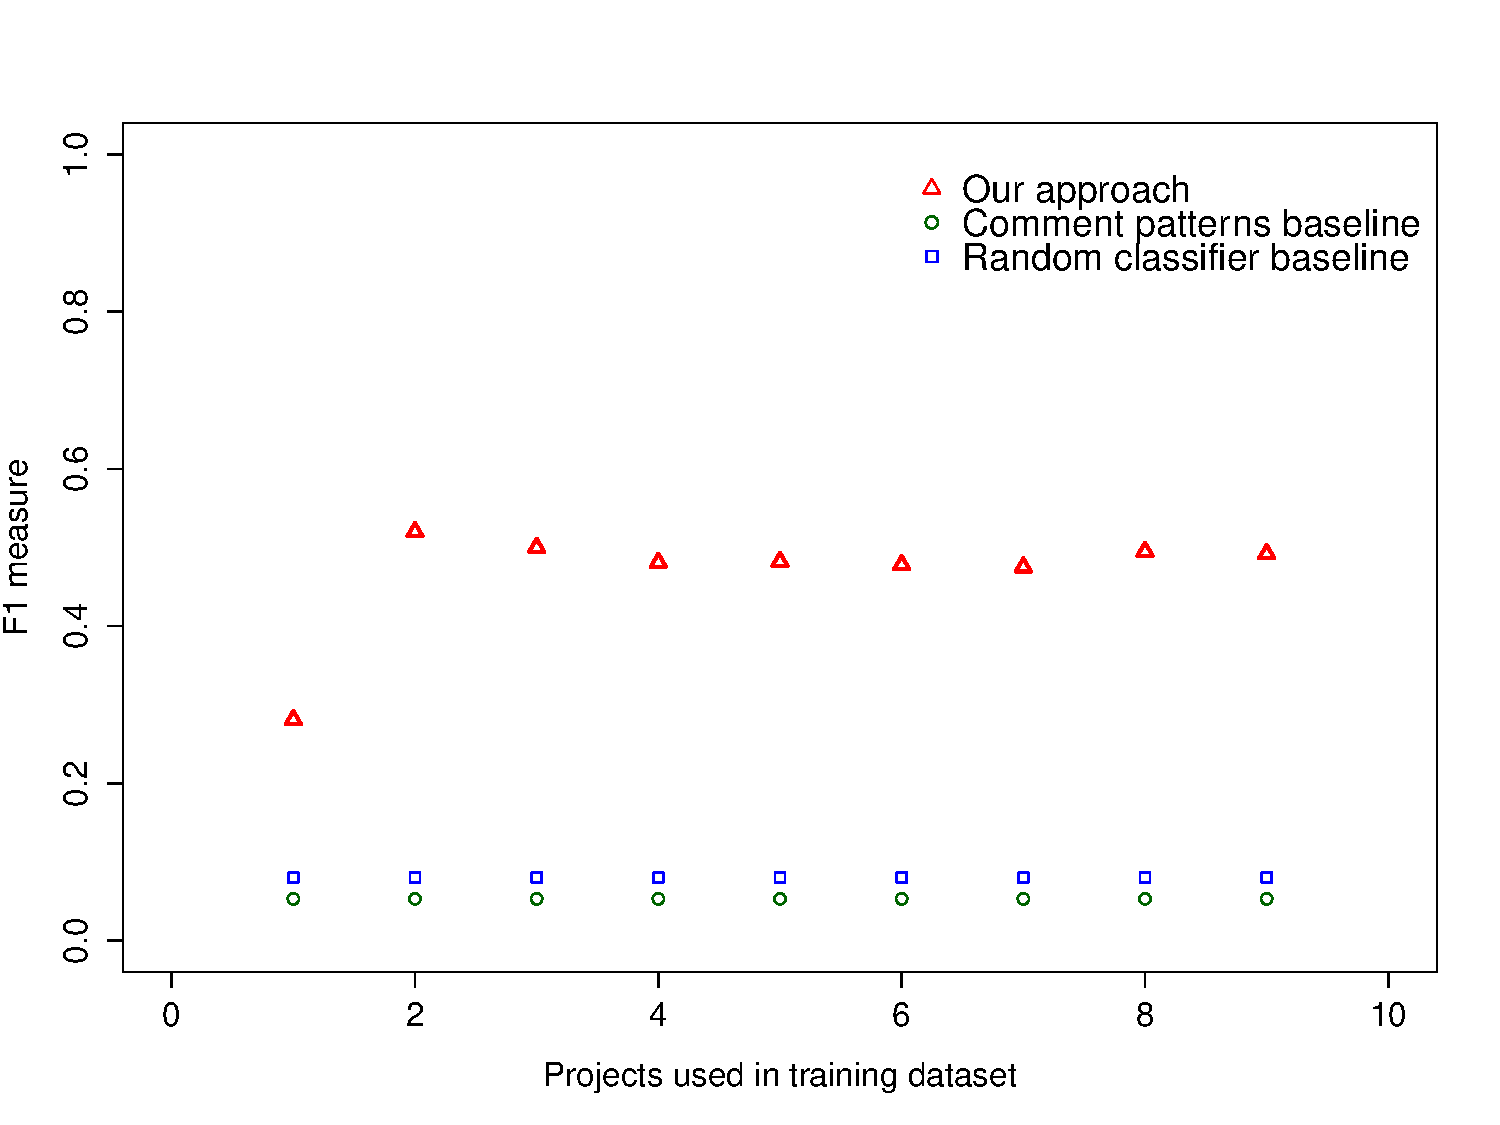
\includegraphics[width=0.49\textwidth]{figures/appendix/iteration_details/design_jfreechart.pdf}
  % \vspace{-3mm}
  \caption{JFreeChart Design Debt Classification}
  \label{fig:design_jfreechart}
\end{figure}

\begin{figure}[thb!]
  \centering
  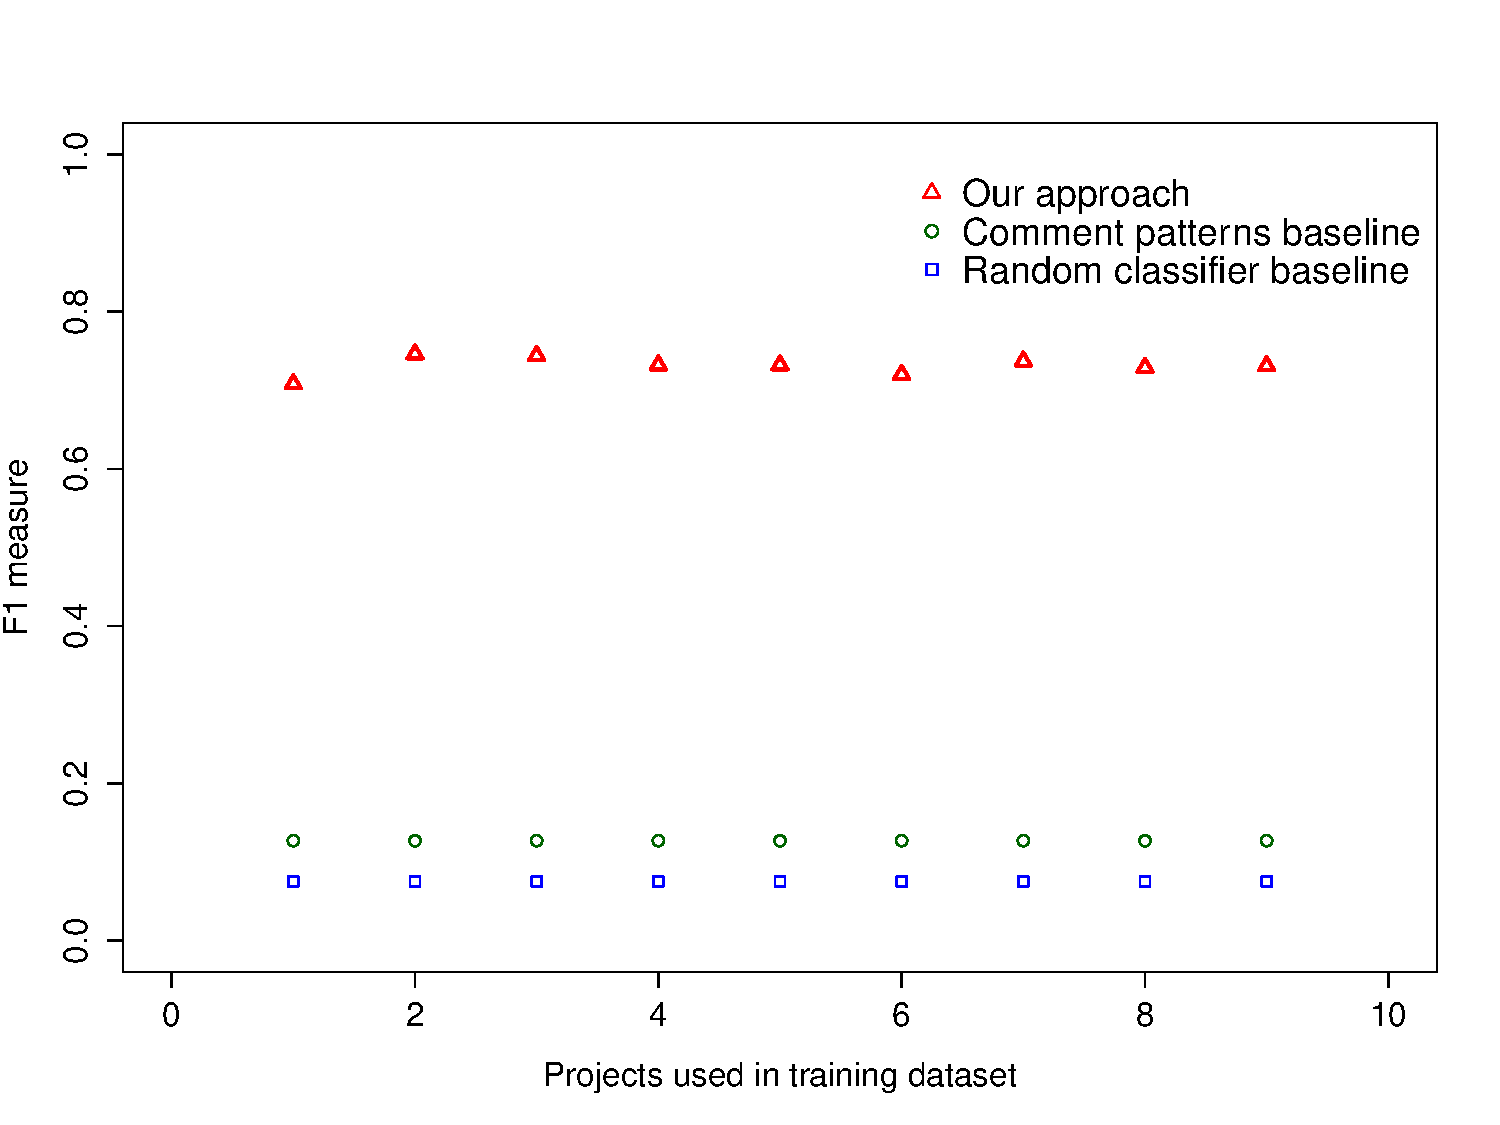
\includegraphics[width=0.49\textwidth]{figures/appendix/iteration_details/design_jmeter.pdf}
  % \vspace{-3mm}
  \caption{Jmeter Design Debt Classification}
  \label{fig:design_jmeter}
\end{figure}

\begin{figure}[thb!]
  \centering
  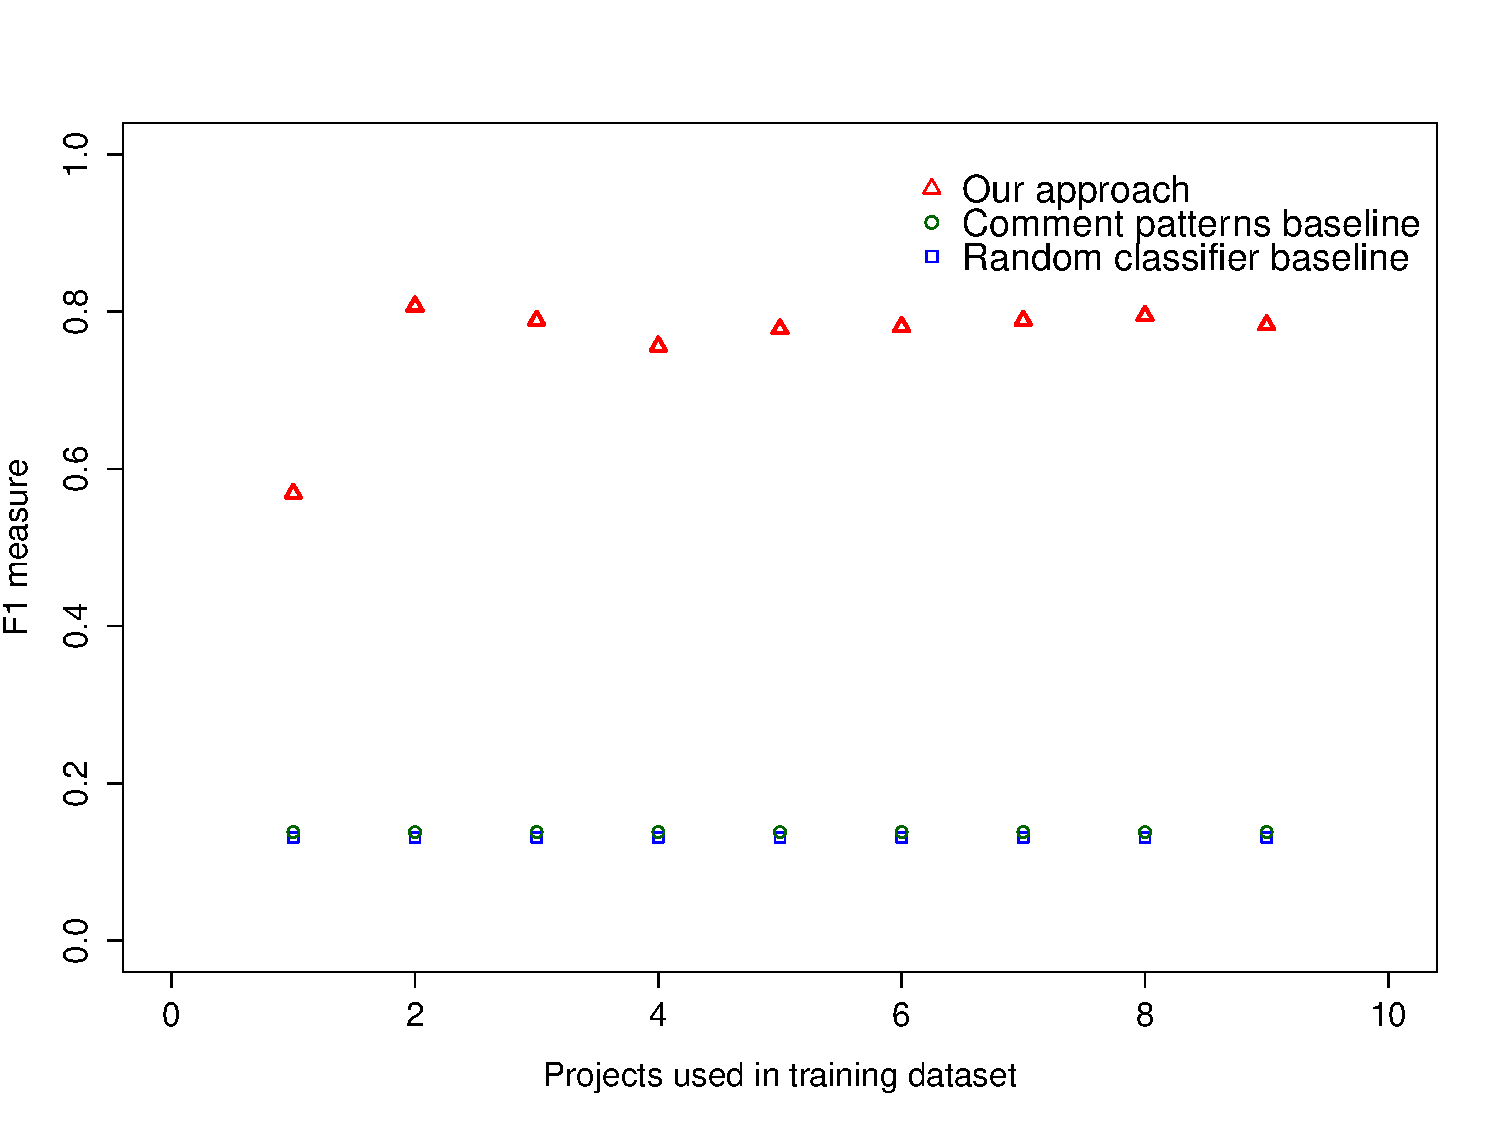
\includegraphics[width=0.49\textwidth]{figures/appendix/iteration_details/design_jruby.pdf}
  % \vspace{-3mm}
  \caption{JRuby Design Debt Classification}
  \label{fig:design_jruby}
\end{figure}

\begin{figure}[thb!]
  \centering
  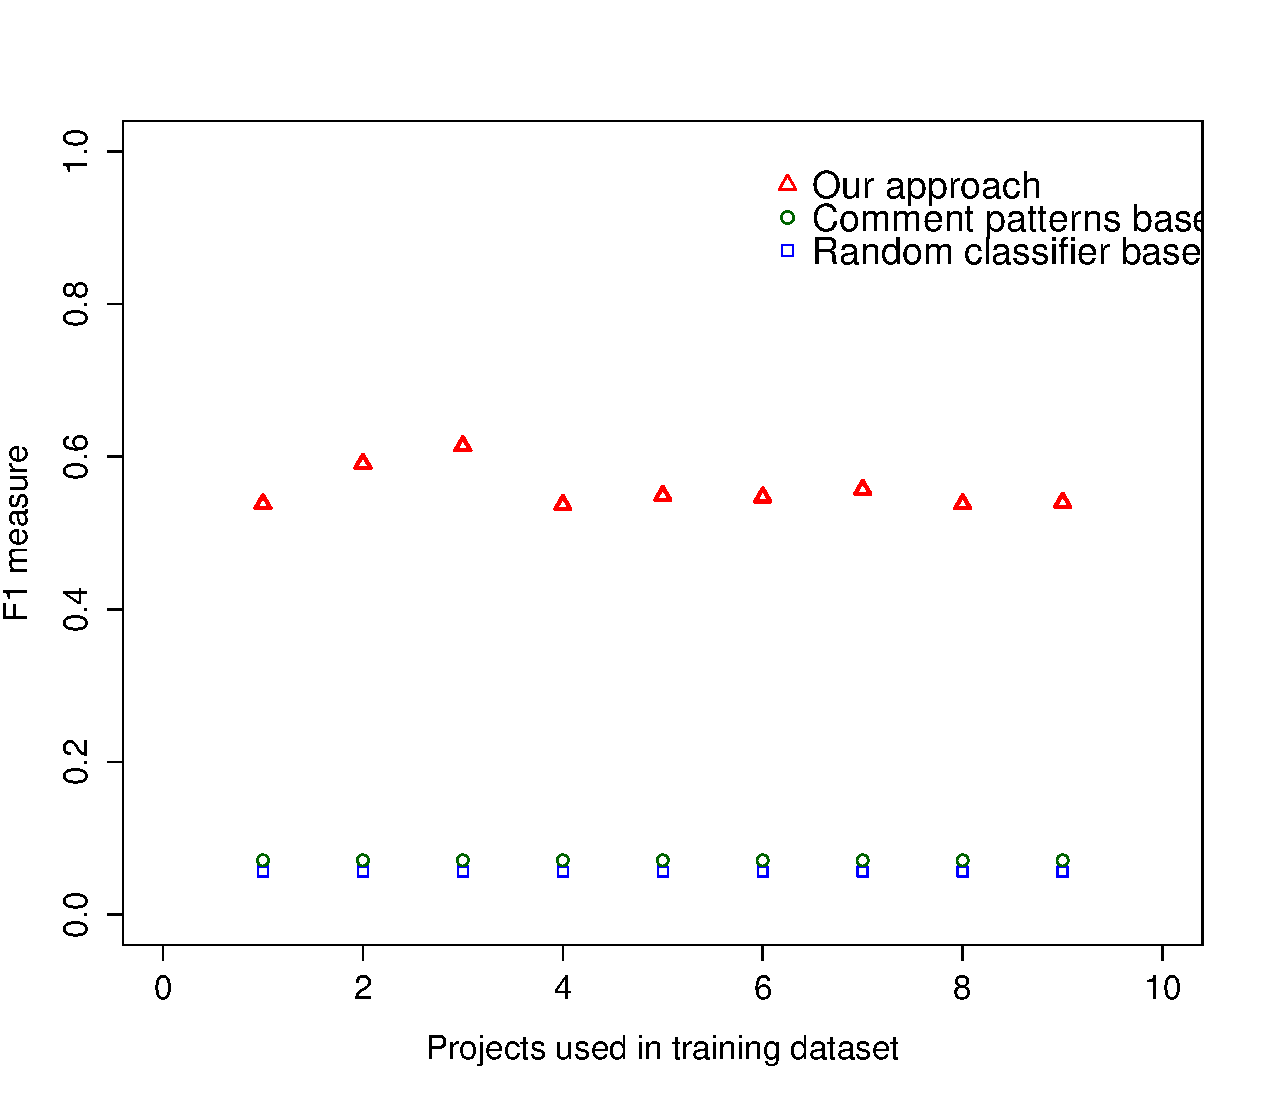
\includegraphics[width=0.49\textwidth]{figures/appendix/iteration_details/design_sql12.pdf}
  % \vspace{-3mm}
  \caption{SQuirrel Design Debt Classification}
  \label{fig:design_sql}
\end{figure}

\clearpage
 
\begin{figure}[thb!]    
  \centering
  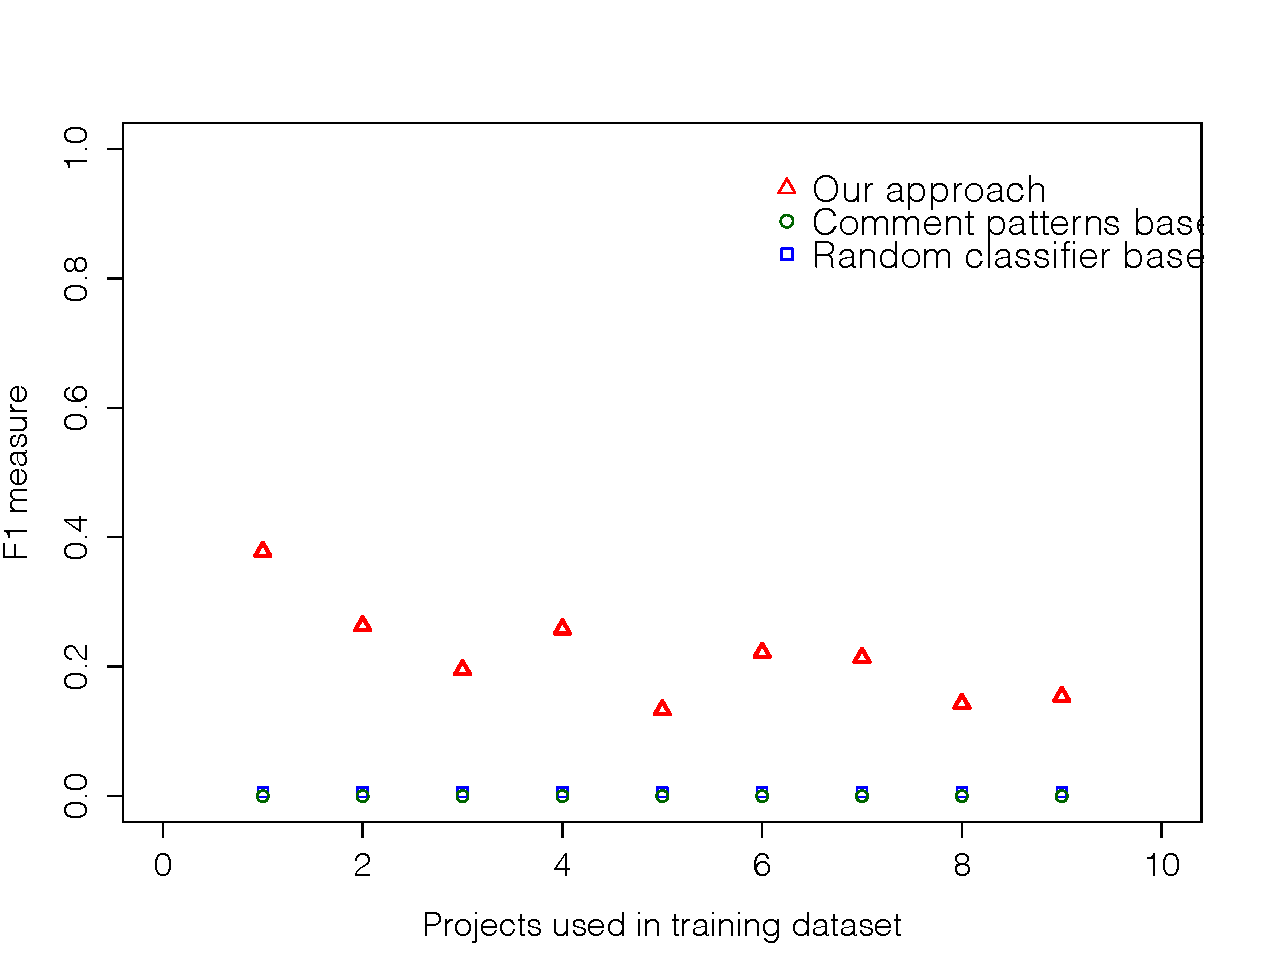
\includegraphics[width=0.49\textwidth]{figures/appendix/iteration_details/implementation_ant.pdf}
  % \vspace{-3mm}
  \caption{Ant Requirement Debt Classification}
  \label{fig:implementation_ant}
\end{figure}

\begin{figure}[thb!]
  \centering
  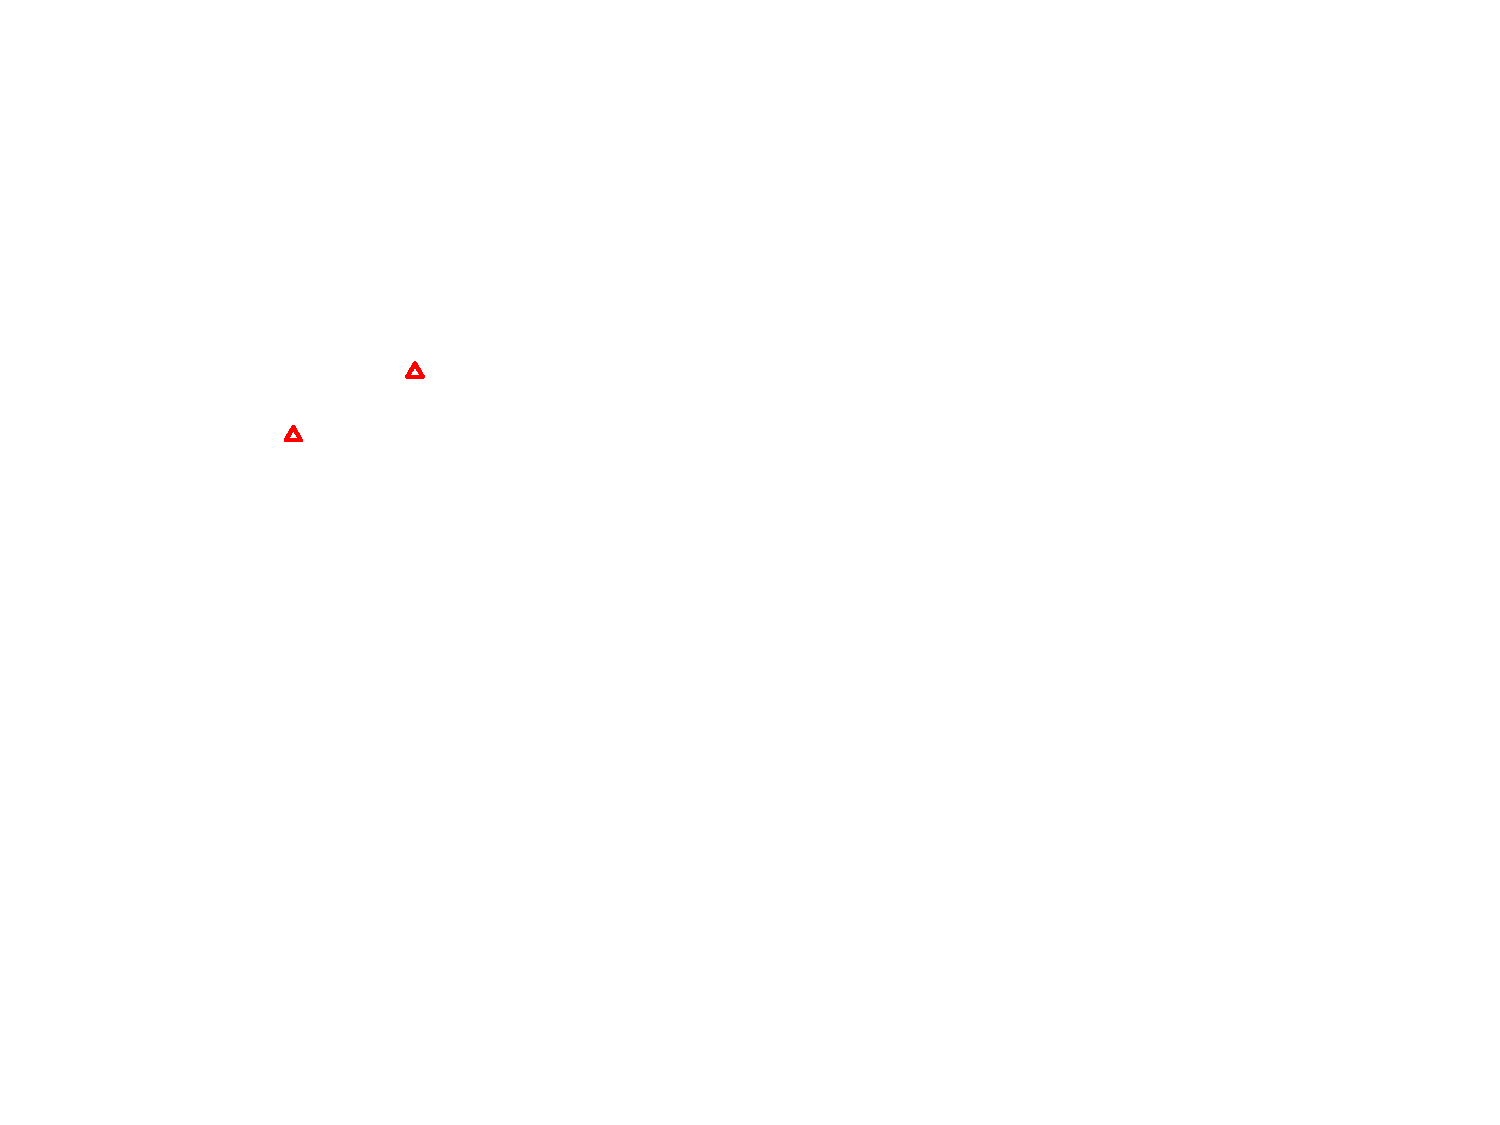
\includegraphics[width=0.49\textwidth]{figures/appendix/iteration_details/implementation_columba.pdf}
  % \vspace{-3mm}
  \caption{Columba Requirement Debt Classification}
  \label{fig:implementation_columba}
\end{figure}

\begin{figure}[thb!]
  \centering
  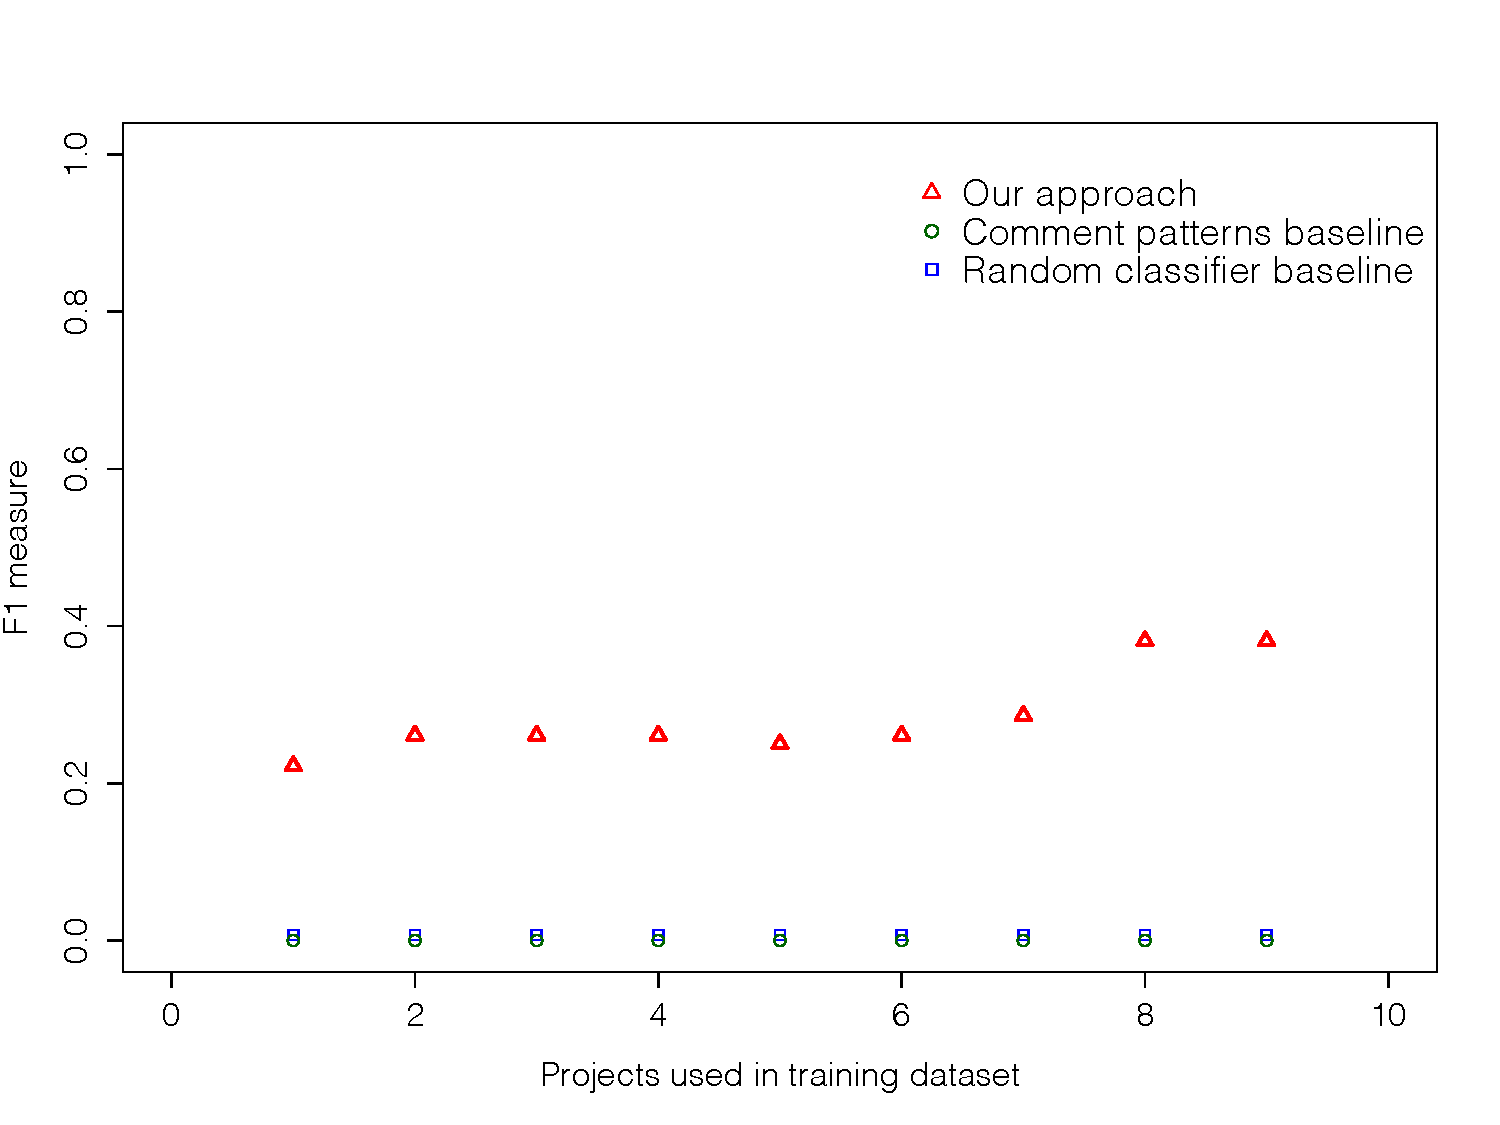
\includegraphics[width=0.49\textwidth]{figures/appendix/iteration_details/implementation_emf.pdf}
  % \vspace{-3mm}
  \caption{Emf Requirement Debt Classification}
  \label{fig:implementation_emf}
\end{figure}

\begin{figure}[thb!]
  \centering
  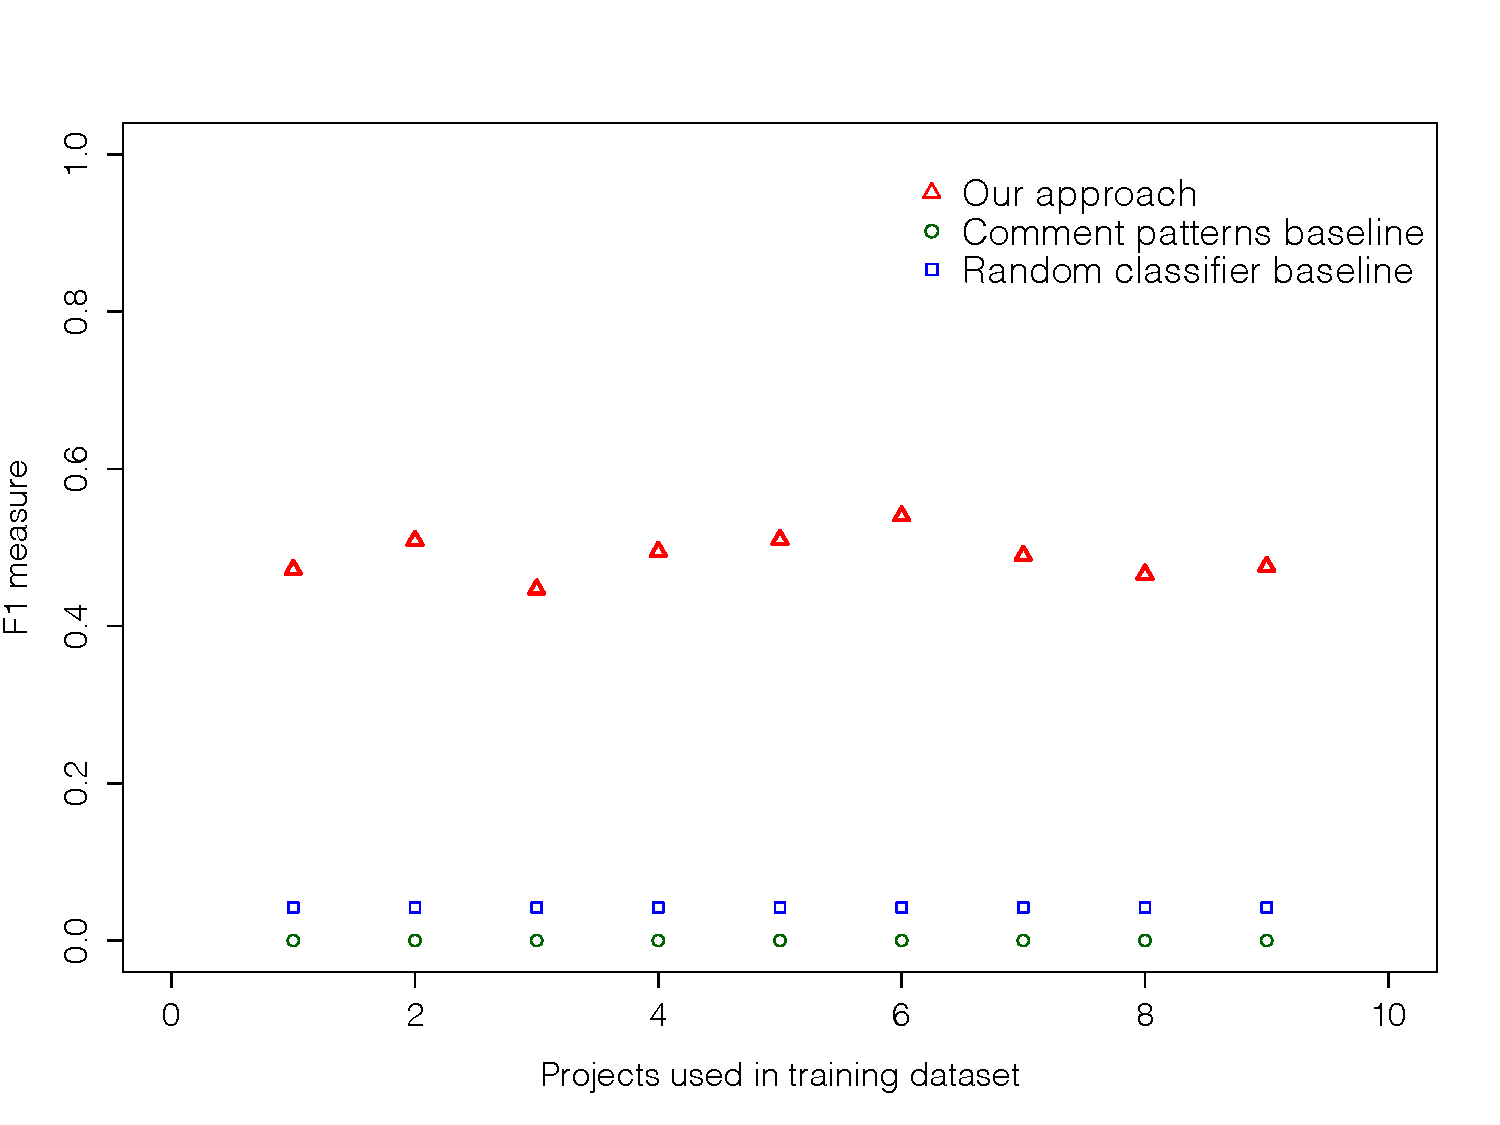
\includegraphics[width=0.49\textwidth]{figures/appendix/iteration_details/implementation_hibernate.pdf}
  \caption{Hibernate Requirement Debt Classification}
  \label{fig:implementation_hibernate}
\end{figure}

\begin{figure}[thb!]
  \centering
  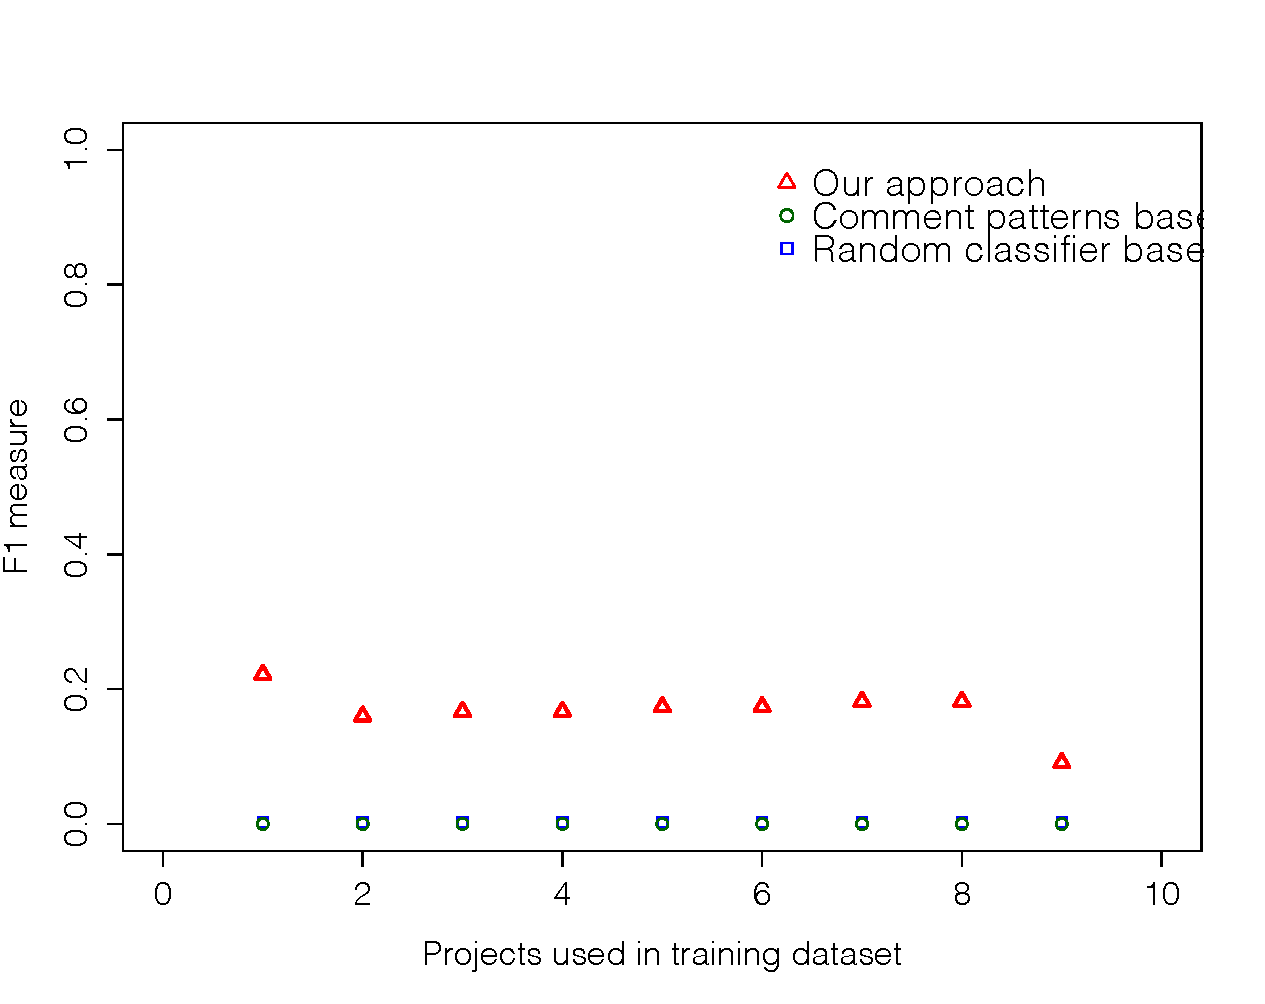
\includegraphics[width=0.49\textwidth]{figures/appendix/iteration_details/implementation_jedit.pdf}
  % \vspace{-3mm}
  \caption{JEdit Requirement Debt Classification}
  \label{fig:implementation_jedit}
\end{figure}

\clearpage

\begin{figure}[thb!]
  \centering
  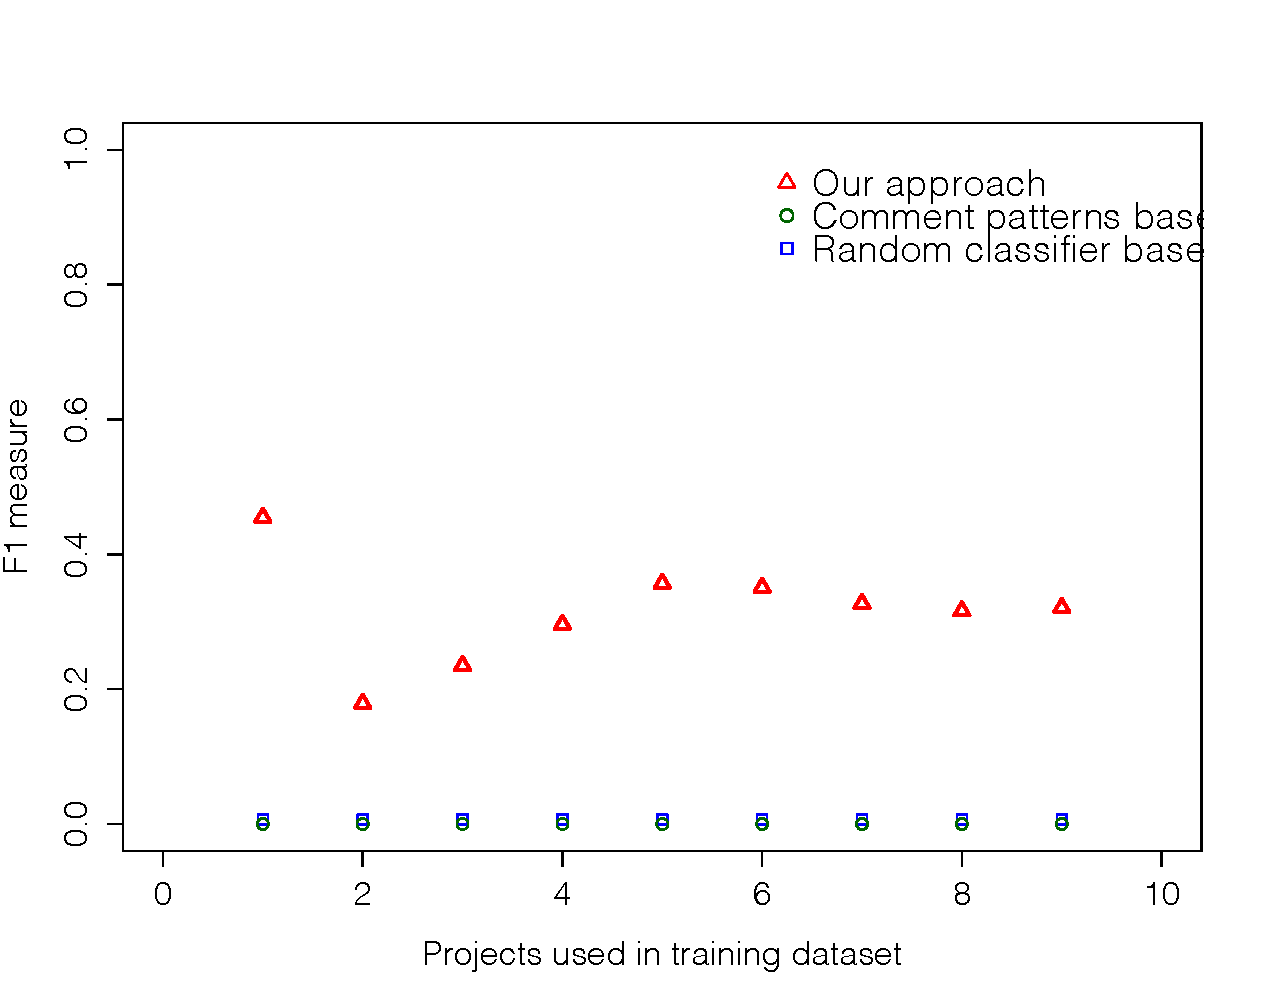
\includegraphics[width=0.49\textwidth]{figures/appendix/iteration_details/implementation_jfreechart.pdf}
  % \vspace{-3mm}
  \caption{JFreeChart Requirement Debt Classification}
  \label{fig:implementation_jfreechart}
\end{figure}

\begin{figure}[thb!]
  \centering
  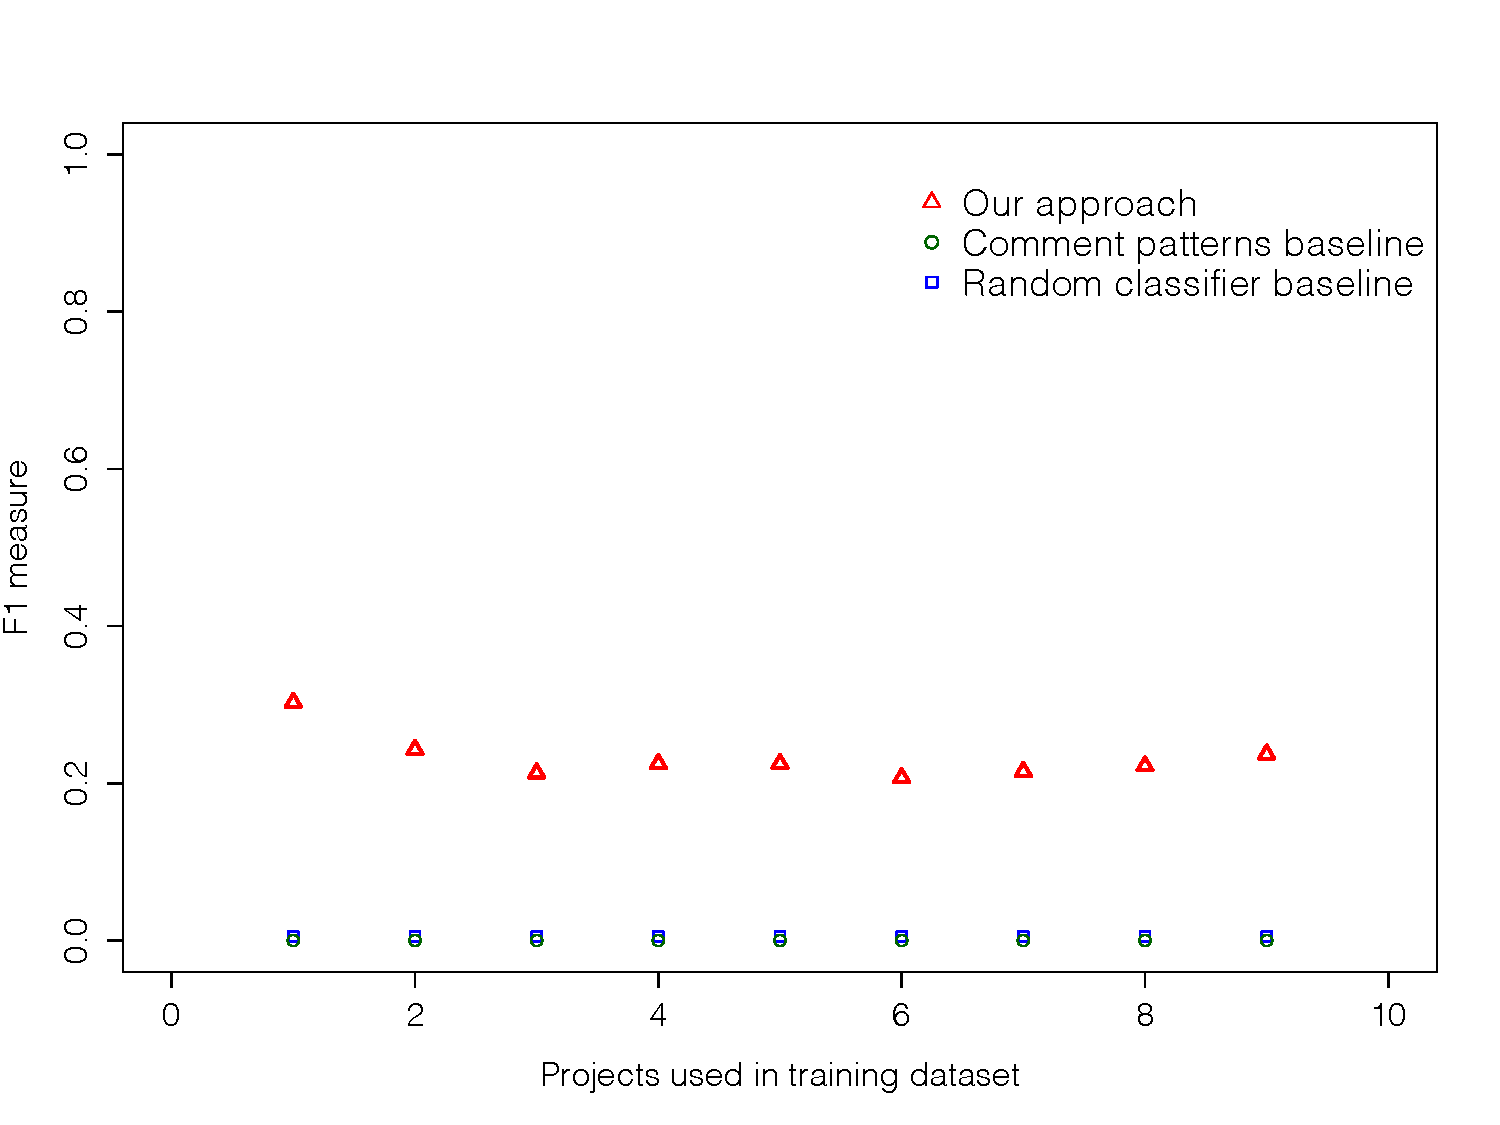
\includegraphics[width=0.49\textwidth]{figures/appendix/iteration_details/implementation_jmeter.pdf}
  % \vspace{-3mm}
  \caption{Jmeter Requirement Debt Classification}
  \label{fig:implementation_jmeter}
\end{figure}

\begin{figure}[thb!]
  \centering
  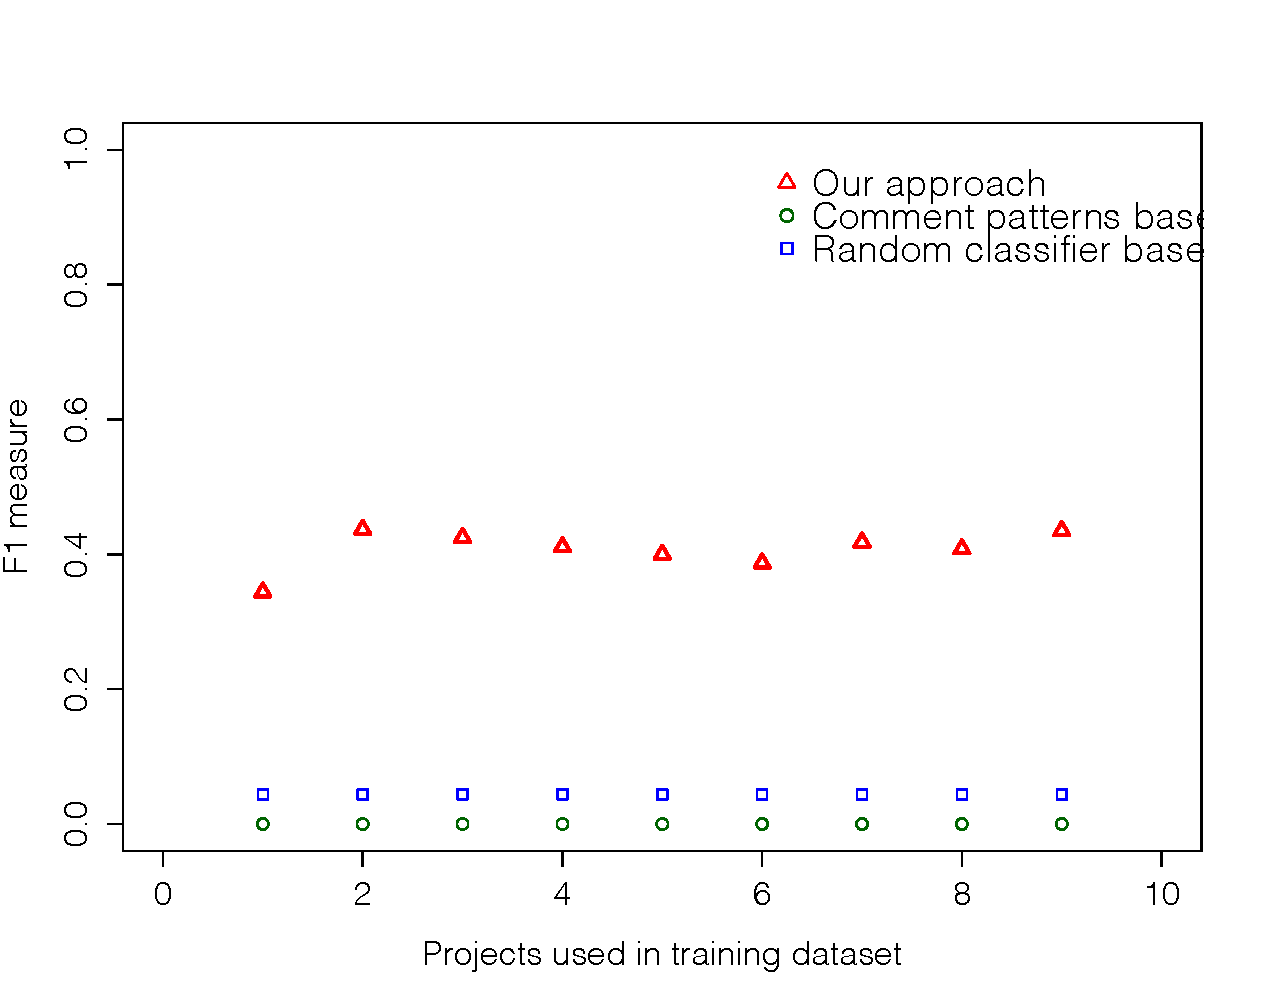
\includegraphics[width=0.49\textwidth]{figures/appendix/iteration_details/implementation_jruby.pdf}
  % \vspace{-3mm}
  \caption{JRuby Requirement Debt Classification}
  \label{fig:implementation_jruby}
\end{figure}

\begin{figure}[thb!]
  \centering
  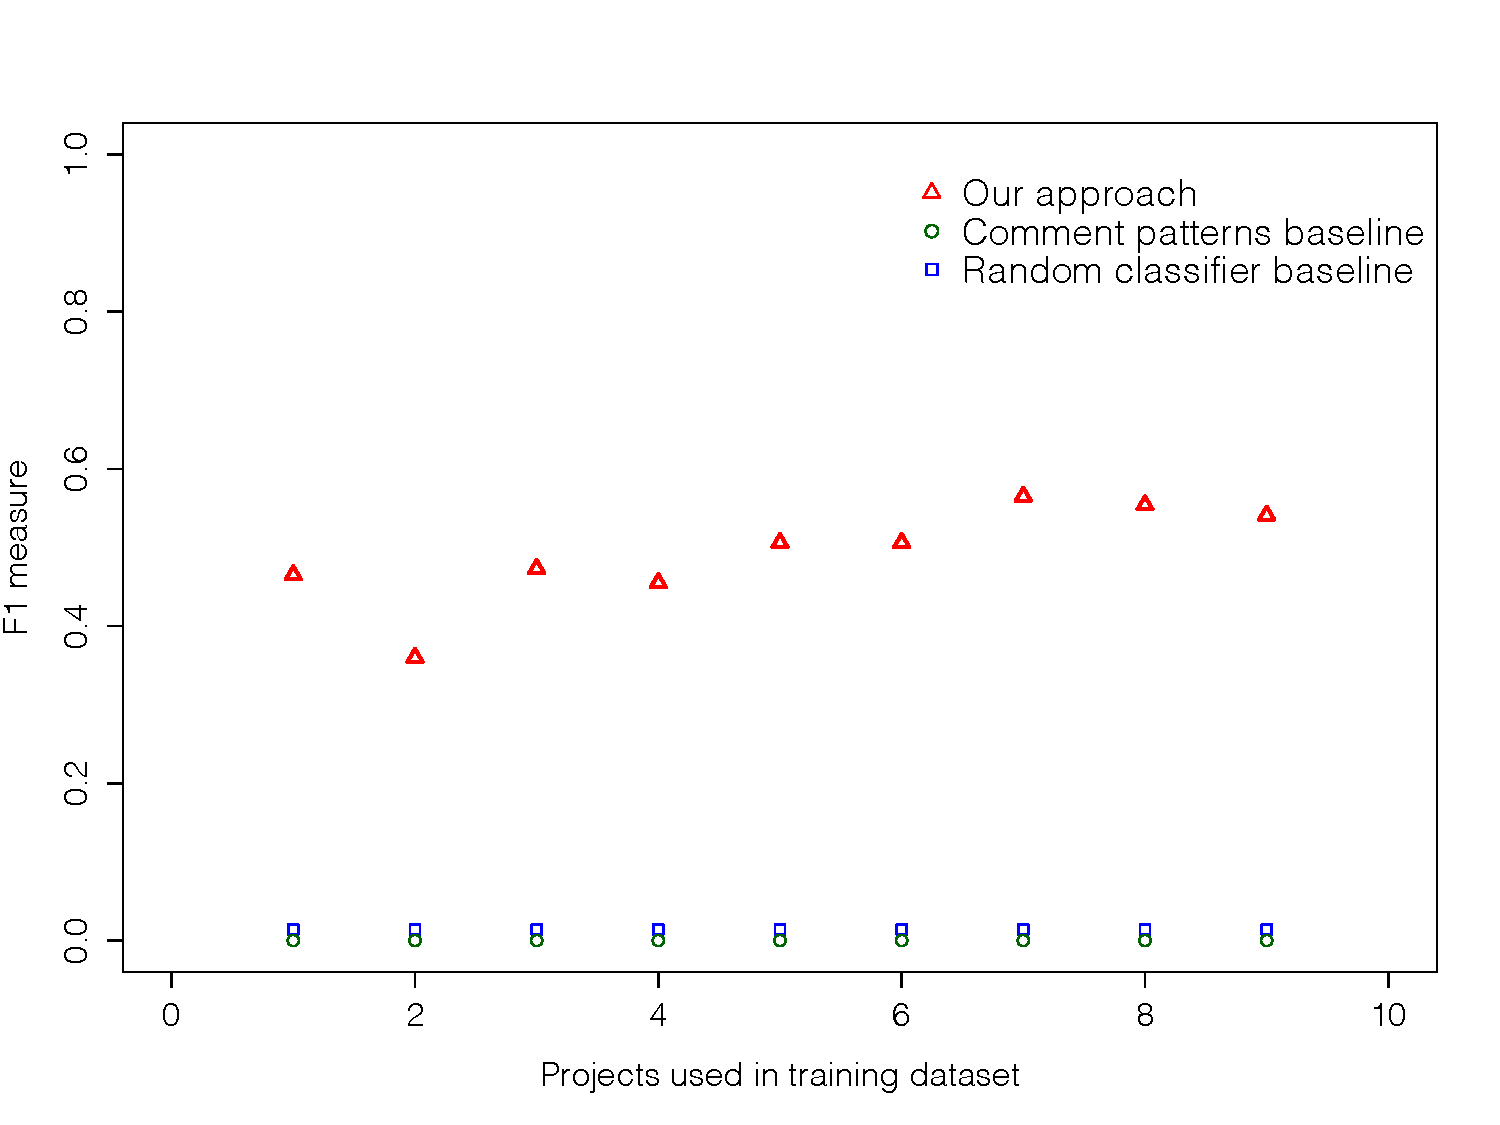
\includegraphics[width=0.49\textwidth]{figures/appendix/iteration_details/implementation_sql12.pdf}
  % \vspace{-3mm}
  \caption{SQuirrel Requirement Debt Classification}
  \label{fig:implementation_sql}
\end{figure}

% \clearpage

% \begin{figure}[thb!]
%   \centering
%   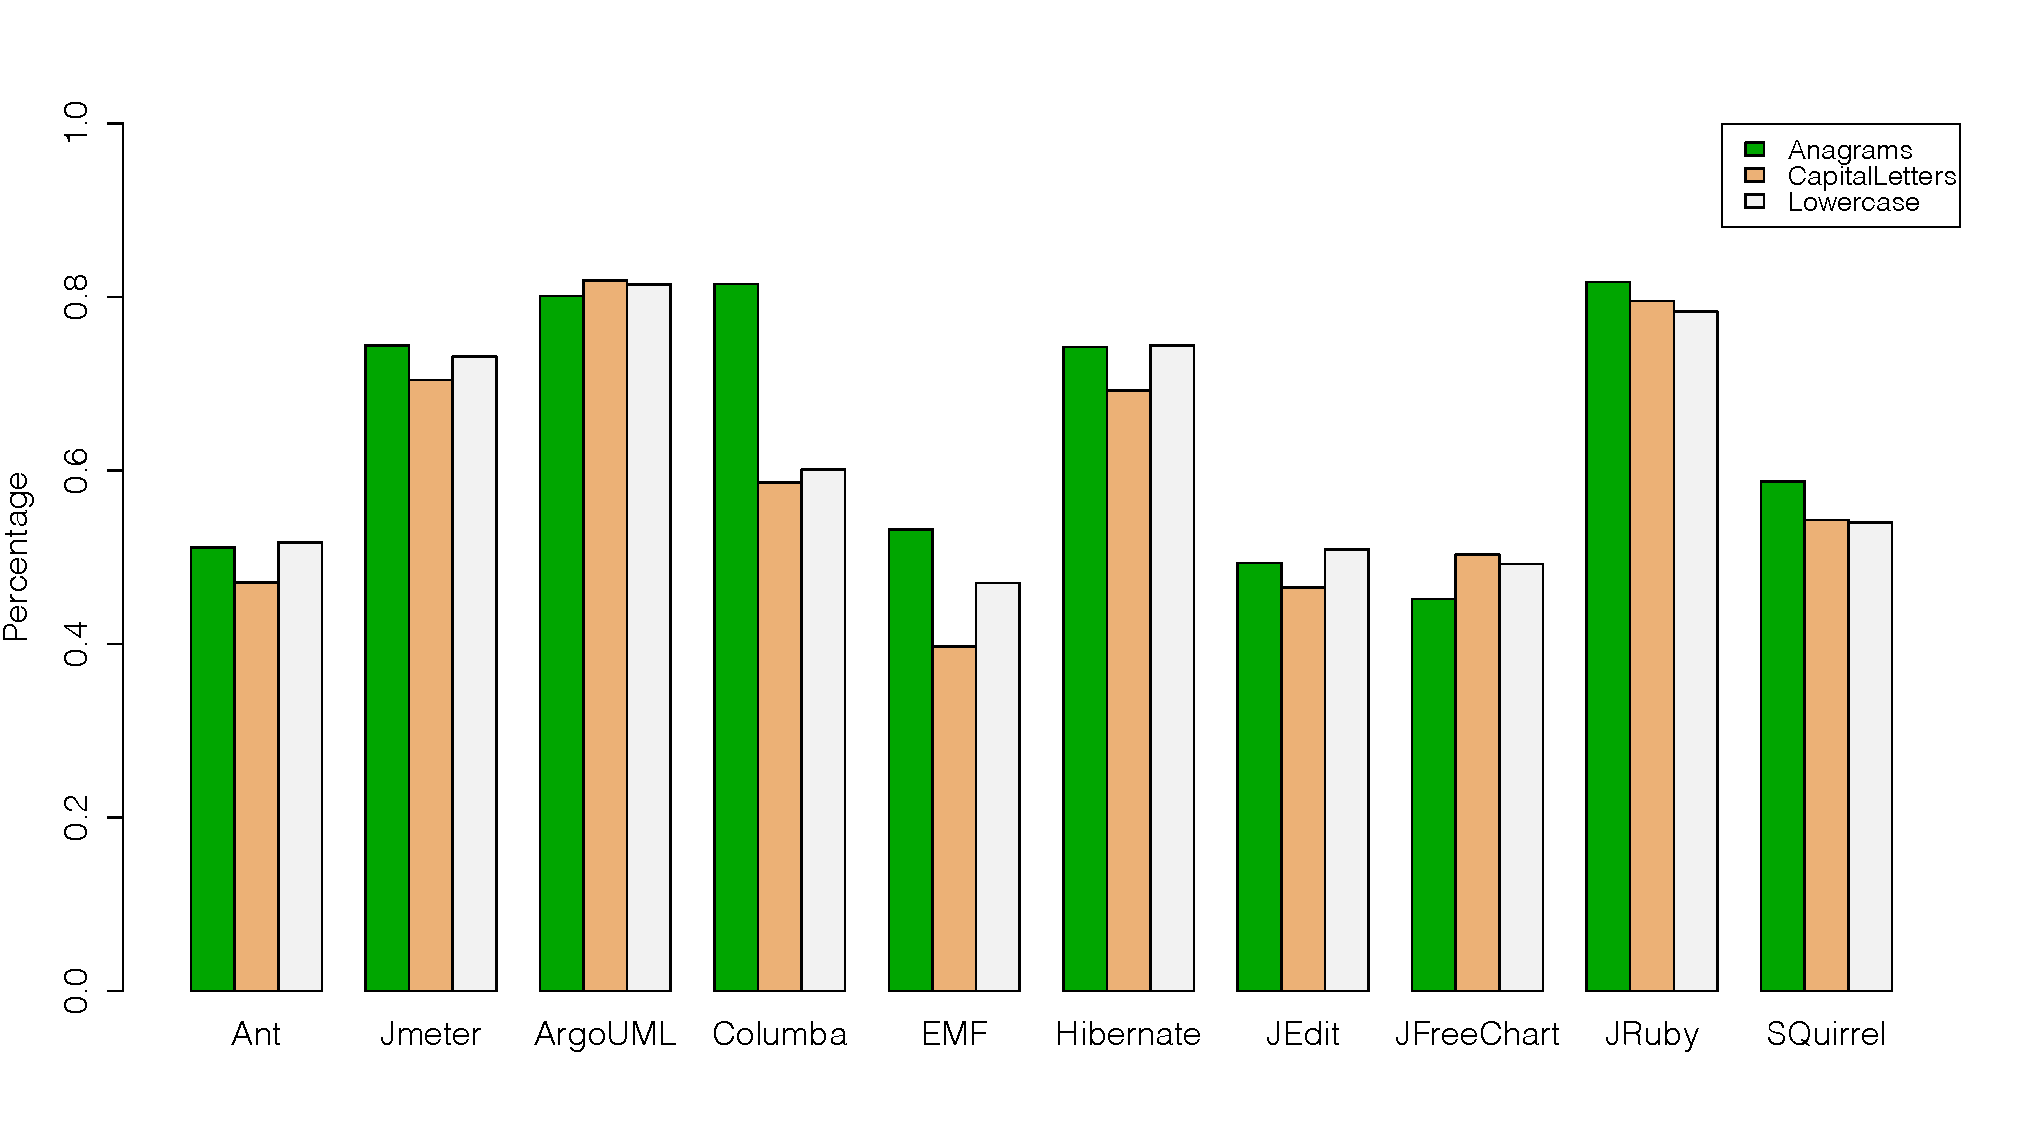
\includegraphics[width=0.50\textwidth]{figures/appendix/detailed_comparison_design_training_dataset.pdf}
%   % \vspace{-3mm}
%   \caption{Detailed comparison of the changes in the design training datasets}
%   \label{fig:detailed_comparison_design_training_dataset}
% \end{figure}

% \begin{figure}[thb!]
%   \centering
%   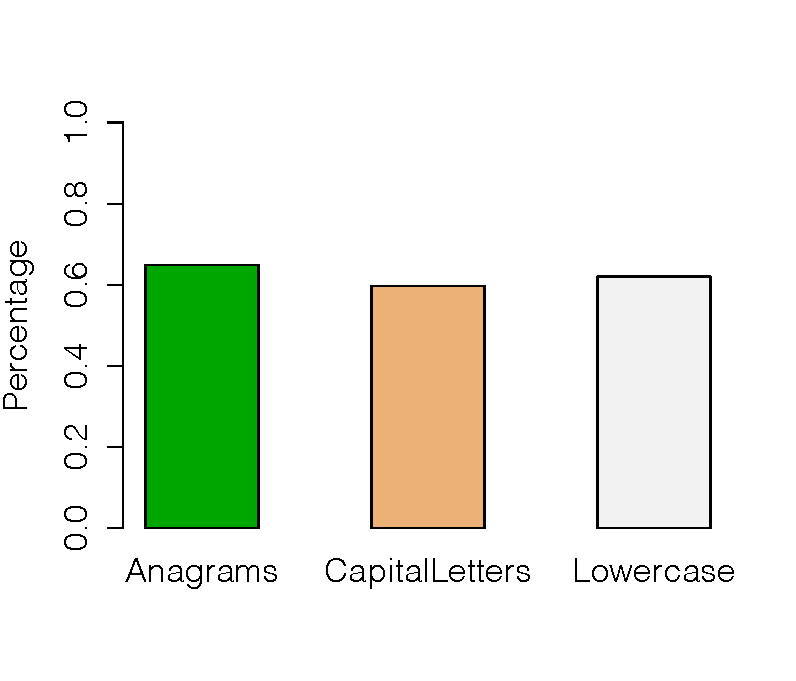
\includegraphics[width=0.50\textwidth]{figures/appendix/average_comparison_design_training_dataset.pdf}
%   % \vspace{-3mm}
%   \caption{Average comparison of the changes in the design training datasets}
%   \label{fig:average_comparison_design_training_dataset}
% \end{figure}

% \begin{table}[!hbt]
%     \begin{center}
%         \caption{Effects in the F1 measure of the Design training datasets}
%         \label{tbl:detailed_comparison_design_training_dataset}
%         \begin{tabular}{l| c c c}
%         \toprule
%         \thead{Project} & \thead{Anagrams\\Dataset} & \thead{Capitalized\\Dataset} & \thead{Lowercase\\Dataset}\\
%         \midrule
%         Apache Ant    &  0.511   & 0.471 &  0.517    \\
%         Apache Jmeter &  0.744   & 0.704 &  0.731    \\
%         ArgoUML       &  0.801   & 0.819 &  0.814    \\
%         Columba       &  0.815   & 0.586 &  0.601    \\
%         EMF           &  0.532   & 0.397 &  0.470    \\
%         Hibernate     &  0.742   & 0.692 &  0.744    \\
%         JEdit         &  0.493   & 0.465 &  0.509    \\
%         JFreeChart    &  0.452   & 0.503 &  0.492    \\
%         JRuby         &  0.817   & 0.795 &  0.783    \\
%         SQuirrel      &  0.587   & 0.543 &  0.540    \\
%         \bottomrule
%         \end{tabular}
%     \end{center}    
% \end{table}

% \clearpage

% \begin{figure}[thb!]
%   \centering
%   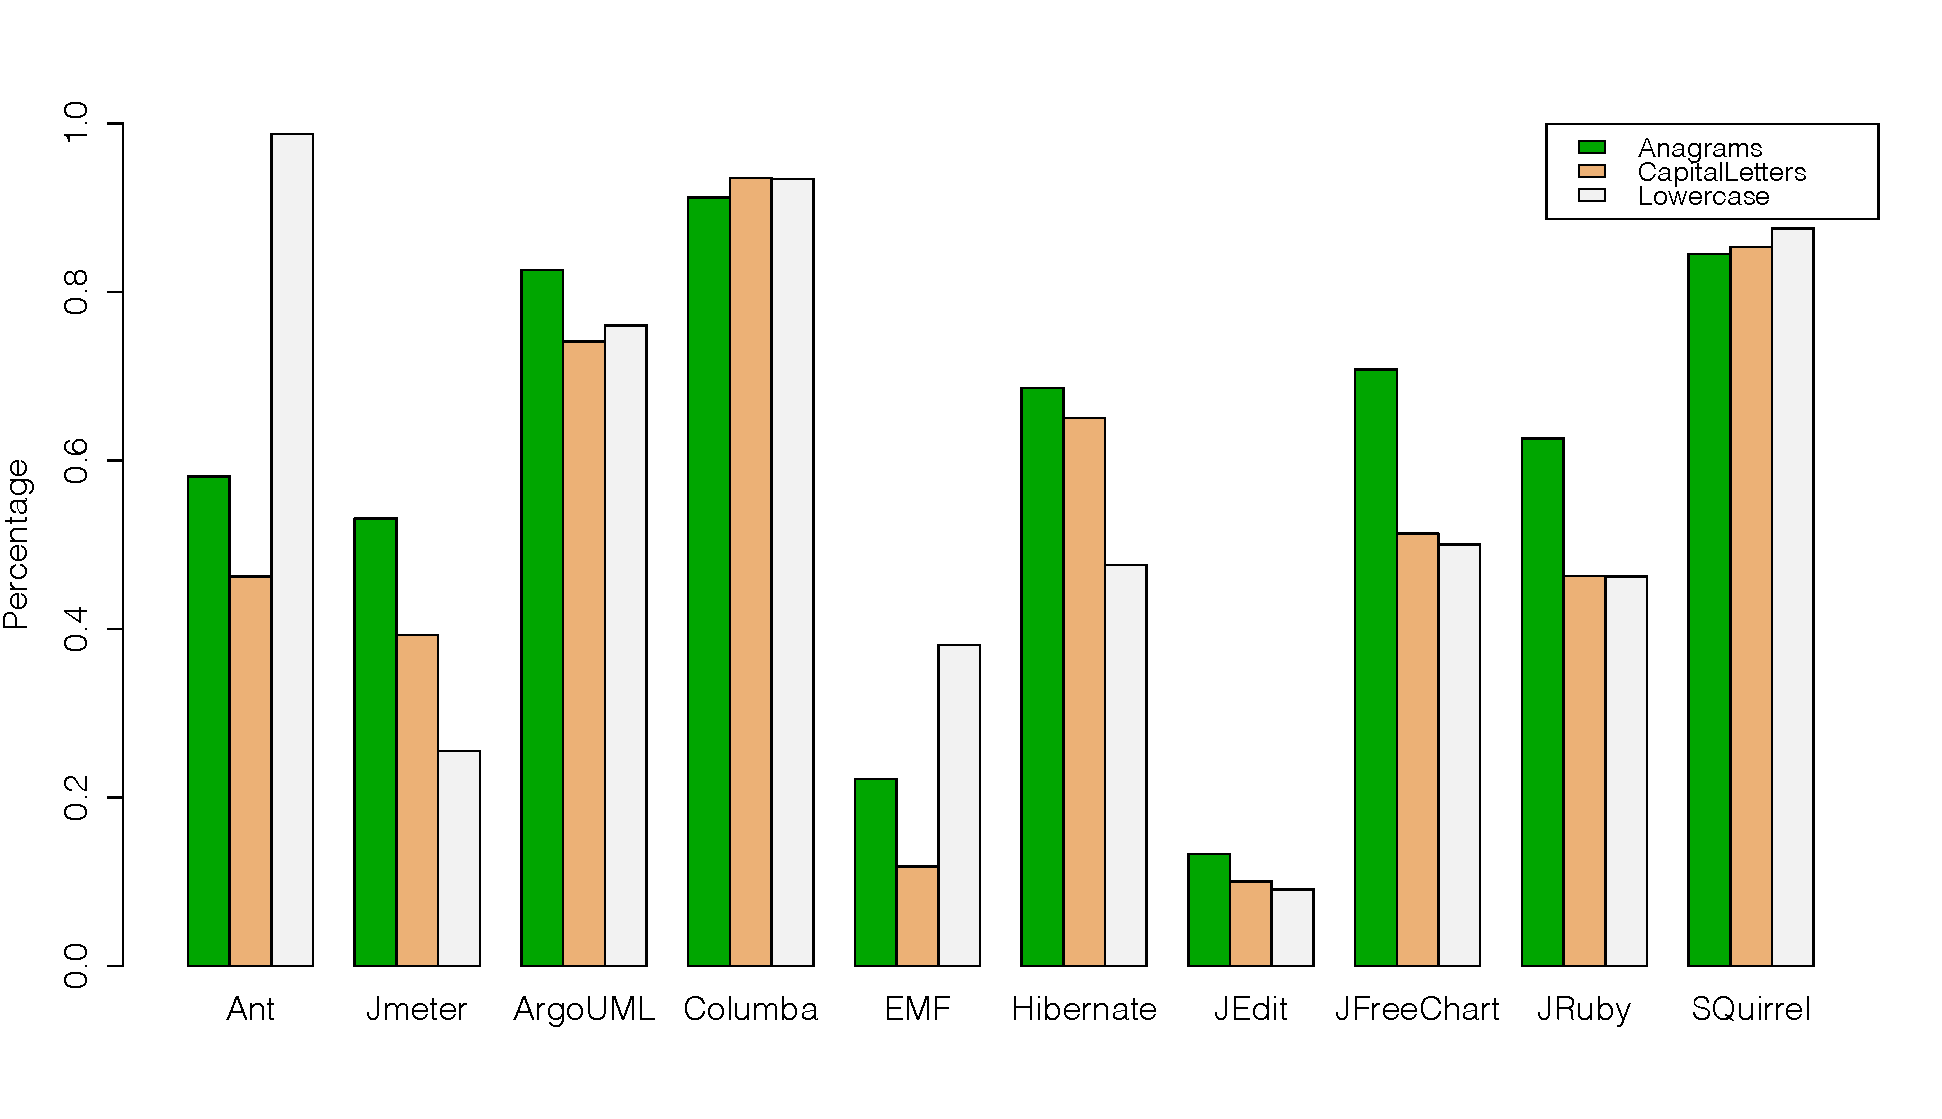
\includegraphics[width=0.50\textwidth]{figures/appendix/detailed_comparison_requirement_training_dataset.pdf}
%   \vspace{-3mm}
%   \caption{Detailed comparison of the changes in the requirements training datasets}
%   \label{fig:detailed_comparison_requirement_training_dataset}
% \end{figure}

% \begin{figure}[thb!]
%   \centering
%   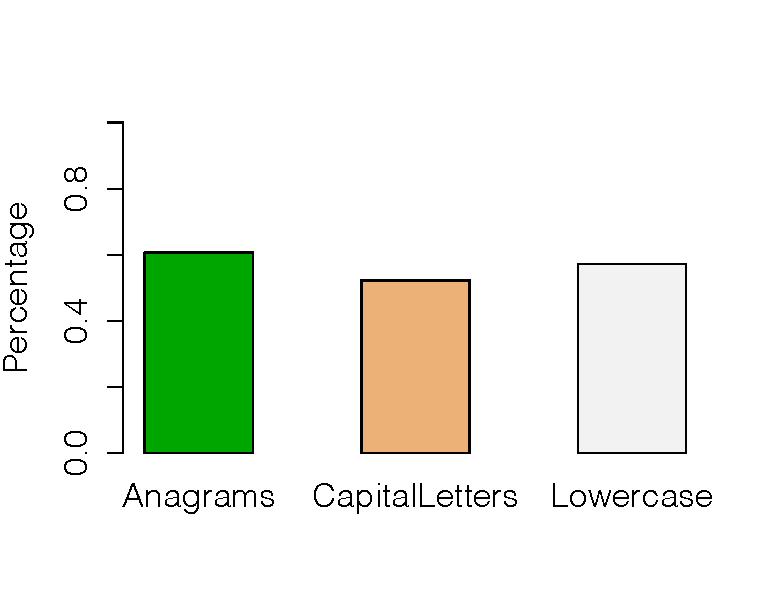
\includegraphics[width=0.50\textwidth]{figures/appendix/average_comparison_requeriment_training_dataset.pdf}
%   \vspace{-3mm}
%   \caption{Average comparison of the changes in the requirements training datasets}
%   \label{fig:average_comparison_requirement_training_dataset}
% \end{figure}

% \begin{table}[!hbt]
%     \begin{center}
%         \caption{Effects in the F1 measure of the Requirements training datasets}
%         \label{tbl:detailed_comparison_requirement_training_dataset}
%         \begin{tabular}{l| c c c}
%         \toprule
%         \thead{Project} & \thead{Anagrams\\Dataset} & \thead{Capitalized\\Dataset} & \thead{Lowercase\\Dataset}\\
%         \midrule
%         Apache Ant    &  0.581 & 0.462 & 0.987  \\
%         Apache Jmeter &  0.531 & 0.393 & 0.255  \\
%         ArgoUML       &  0.826 & 0.741 & 0.760  \\
%         Columba       &  0.912 & 0.935 & 0.934  \\
%         EMF           &  0.222 & 0.118 & 0.381  \\
%         Hibernate     &  0.686 & 0.650 & 0.476  \\
%         JEdit         &  0.133 & 0.100 & 0.091  \\
%         JFreeChart    &  0.708 & 0.513 & 0.500  \\
%         JRuby         &  0.626 & 0.463 & 0.462  \\
%         SQuirrel      &  0.845 & 0.853 & 0.875  \\
%         \bottomrule
%         \end{tabular}
%     \end{center}    
% \end{table}


\clearpage
\subsection*{Detailed Precision and Recall Values When Different Underlying Classifiers are Used}

When presenting the results in Section~\ref{sec:underlying_classifier}, we only presented the F1-measures. Here, we present the detailed precision and recall values that make up the F1-measures presented earlier.

\begin{table*}[!thb]
    \begin{center}
        \caption{Comparison Between Different Classifiers Algorithms for Design Debt}
        \label{tbl:improvement_f1measure_between_classifiers_design}
        \begin{tabular}{l| c c c|| c c c|| c c c }
        \toprule

        \multirow{4}{*}{\textbf{\thead{Project}}} & \multicolumn{3}{c||}{\textbf{\thead{Logistic Regression}}} & \multicolumn{3}{c||}{\textbf{\thead{Naive Bayes}}} & \multicolumn{3}{c}{\textbf{\thead{Binary}}} 
        
        \\ 
        \cmidrule{2-10}
        
        & \textbf{\thead{Precision}} & \textbf{\thead{Recall}} & \textbf{\thead{F1 measure}} & \textbf{\thead{Precision}} & \textbf{\thead{Recall}} & \textbf{\thead{F1 measure}} & \textbf{\thead{Precision}} & \textbf{\thead{Recall}} & \textbf{\thead{F1 measure}}\\
        \midrule                                                  
        \textbf{Ant}          &  0.554 & 0.484 &  0.517 &  0.072 & 0.874 & 0.134 &  0.620 & 0.516 & 0.563  \\
        \textbf{ArgoUML}      &  0.788 & 0.843 &  0.814 &  0.358 & 0.985 & 0.525 &  0.790 & 0.858 & 0.822  \\
        \textbf{Columba}      &  0.792 & 0.484 &  0.601 &  0.181 & 0.786 & 0.294 &  0.840 & 0.500 & 0.627  \\
        \textbf{EMF}          &  0.574 & 0.397 &  0.470 &  0.057 & 0.872 & 0.106 &  0.633 & 0.397 & 0.488  \\
        \textbf{Hibernate}    &  0.877 & 0.645 &  0.744 &  0.288 & 0.890 & 0.435 &  0.895 & 0.670 & 0.767  \\
        \textbf{JEdit}        &  0.779 & 0.378 &  0.509 &  0.227 & 0.791 & 0.353 &  0.807 & 0.342 & 0.480  \\
        \textbf{JFreeChart}   &  0.646 & 0.397 &  0.492 &  0.140 & 0.560 & 0.224 &  0.658 & 0.397 & 0.495  \\
        \textbf{Jmeter}       &  0.808 & 0.668 &  0.731 &  0.224 & 0.801 & 0.350 &  0.819 & 0.671 & 0.737  \\
        \textbf{JRuby}        &  0.798 & 0.770 &  0.783 &  0.275 & 0.971 & 0.429 &  0.815 & 0.808 & 0.811  \\
        \textbf{SQuirrel}     &  0.544 & 0.536 &  0.540 &  0.133 & 0.947 & 0.233 &  0.567 & 0.550 & 0.558  \\
        \midrule                                                  
        \textbf{Average}      &  0.716 &   0.5602 &  0.6201 &  0.1955  & 0.8477  & 0.3083 & 0.7444  & 0.5709 & 0.6348  \\
        \bottomrule
        \end{tabular}
    \end{center}    
\end{table*}

\begin{table*}[!thb]
    \begin{center}
        \caption{Comparison Between Different Classifiers Algorithms for Requirement Debt}
        \label{tbl:improvement_f1measure_between_classifiers_requirement}
        \begin{tabular}{l| c c c|| c c c|| c c c }
        \toprule
        \multirow{4}{*}{\textbf{\thead{Project}}} & \multicolumn{3}{c||}{\textbf{\thead{Logistic Regression}}} & \multicolumn{3}{c||}{\textbf{\thead{Naive Bayes}}} & \multicolumn{3}{c}{\textbf{\thead{Binary}}} 
        
        \\ 
        \cmidrule{2-10}
        
        & \textbf{\thead{Precision}} & \textbf{\thead{Recall}} & \textbf{\thead{F1 measure}} & \textbf{\thead{Precision}} & \textbf{\thead{Recall}} & \textbf{\thead{F1 measure}} & \textbf{\thead{Precision}} & \textbf{\thead{Recall}} & \textbf{\thead{F1 measure}}\\
        \midrule                                                  
        \textbf{Ant}          &  0.154 & 0.154 & 0.154 & 0.007 &  0.769 & 0.013 & 0.188 & 0.231 & 0.207 \\
        \textbf{ArgoUML}      &  0.663 & 0.540 & 0.595 & 0.119 &  0.808 & 0.207 & 0.659 & 0.569 & 0.611 \\
        \textbf{Columba}      &  0.755 & 0.860 & 0.804 & 0.030 &  0.930 & 0.057 & 0.755 & 0.860 & 0.804 \\
        \textbf{EMF}          &  0.800 & 0.250 & 0.381 & 0.009 &  1.000 & 0.018 & 0.800 & 0.250 & 0.381 \\
        \textbf{Hibernate}    &  0.610 & 0.391 & 0.476 & 0.041 &  0.781 & 0.078 & 0.615 & 0.375 & 0.466 \\
        \textbf{JEdit}        &  0.125 & 0.071 & 0.091 & 0.011 &  0.857 & 0.022 & 0.143 & 0.071 & 0.095 \\
        \textbf{JFreeChart}   &  0.220 & 0.600 & 0.321 & 0.009 &  0.800 & 0.018 & 0.179 & 0.467 & 0.259 \\
        \textbf{Jmeter}       &  0.153 & 0.524 & 0.237 & 0.011 &  0.952 & 0.022 & 0.180 & 0.524 & 0.268 \\
        \textbf{JRuby}        &  0.686 & 0.318 & 0.435 & 0.058 &  0.836 & 0.109 & 0.679 & 0.327 & 0.442 \\
        \textbf{SQuirrel}     &  0.657 & 0.460 & 0.541 & 0.018 &  0.900 & 0.036 & 0.455 & 0.500 & 0.476 \\
        \midrule                                                  
        \textbf{Average}      & 0.4823 &  0.4168 & 0.4035 & 0.0313 & 0.8633 & 0.058  & 0.4653 & 0.4174 & 0.4009 \\
        \bottomrule
        \end{tabular}
    \end{center}    
\end{table*} 


\end{document}